
\documentclass[a4paper, 12pt, svgnames]{report}
%\documentclass[a4paper, 12pt, svgnames, twoside, openright]{report}

\usepackage[francais]{babel}
\usepackage[utf8x]{inputenc}
\usepackage[T1]{fontenc}
\usepackage{graphicx,color}
\usepackage{hyperref}
\usepackage{vmargin}
\usepackage{listings}
\usepackage{caption}
\usepackage{fancyhdr}
\usepackage{lastpage}
\usepackage{tabularx}
\usepackage{longtable}
\usepackage{afterpage} 
\usepackage[final]{pdfpages}
\usepackage[nowarn,style=super3colheader,acronym]{glossaries}
\usepackage{glossary-super}
\usepackage{lipsum}
\usepackage{placeins}
\usepackage{float}
\usepackage{dirtree}
\usepackage{multirow}
\usepackage{libertine}
\usepackage[svgnames]{xcolor}
\usepackage{framed}
\usepackage{epigraph}
\usepackage[babel=true]{csquotes}
\usepackage{url}
\usepackage{pdfpages}

\makeglossaries

%!TEX root = ../report.tex

%
%variables·
%
\def\authornameone{Alan Brunetti}
\def\authormailone{alan.brunetti@edu.hefr.ch}


\def\supervisornameb{Jean-Frédéric Wagen}
\def\supervisormailb{jean-frederic.wagen@hefr.ch}

\def\supervisornamec{Jean-Roland Schuler}
\def\supervisormailc{jean-roland.schuler@hefr.ch}


\def\organisationdepartment{Filière informatique}

\def\documenttitle{Qualité de service entre Set-Top Box et routeur}
\def\documenttype{Rapport de projet}

\def\modulename{Cahier des charges}

\def\subjectName{QoS for STB on Android}
\def\reportdate{\today}
\def\classid{I3}
\def\docversion{1.0}
\def\reportpdftitle{\subjectName}


\definecolor{listinglightgray}{gray}{0.95}
\definecolor{listinggray}{gray}{0.4}
\definecolor{listinggreen}{rgb}{0,0.5,0}
%!TEX root = ../rapport.tex

\hypersetup{
  pdfauthor = {\authornameone},
  pdftitle = {\reportpdftitle},
  pdfsubject = {\modulename, \documenttitle},
  unicode=false,		  % non-Latin characters in Acrobat’s bookmarks
  pdftoolbar=true,		  % show Acrobat’s toolbar?
  pdfmenubar=true,		  % show Acrobat’s menu?
  pdffitwindow=false,	  % window fit to page when opened
  pdfstartview={FitH},	  % fits the width of the page to the window
  pdfcreator={LaTeX},	  % creator of the document
  pdfproducer={latexpdf}, % producer of the document
  pdfkeywords={Report},	  % list of keywords
  pdfnewwindow=true,	  % links in new window
  colorlinks=true,		  % false: boxed links; true: colored links
  linkcolor=black,		  % color of internal links
  citecolor=black,		  % color of links to bibliography
  filecolor=blue,		  % color of file links
  urlcolor=black,		  % color of external links
  linktoc=all
}

\setmargins{2.5cm}%		% left edge
		   {1.5cm}%		% top edge
		   {15.5cm}%	% text width
		   {23.42cm}%	% text hight
		   {14pt}%		% header hight
		   {1cm}%		% header distance
		   {0pt}%		% footer hight
		   {2cm}%		% footer distance

\lstset{
	basicstyle=\footnotesize\ttfamily, % Standardschrift
	numbers=left,				% Ort der Zeilennummern
	numberstyle=\tiny,			% Stil der Zeilennummern
	stepnumber=1,				% Abstand zwischen den Zeilennummern
	numbersep=5pt,				% Abstand der Nummern zum Text
	tabsize=2,					% Groesse von Tabs
	extendedchars=true,			%
	breaklines=true,			% Zeilen werden Umgebrochen
	keywordstyle=\color{blue},
	frame=b,		
	keywordstyle=[1]\textbf,	% Stil der Keywords
	keywordstyle=[2]\textbf,	%
	keywordstyle=[3]\textbf,	%
	keywordstyle=[4]\textbf	  %\sqrt{\sqrt{}} %
	stringstyle=\color{blue}\ttfamily, % Farbe der String
	showspaces=false,			% Leerzeichen anzeigen ?
	showtabs=false,				% Tabs anzeigen ?
	xleftmargin=17pt,
	framexleftmargin=17pt,
	framexrightmargin=0pt,
	framexbottommargin=4pt,
	backgroundcolor=\color{listinglightgray},
	showstringspaces=false,		 % Leerzeichen in Strings anzeigen ?	
	commentstyle=\color{listinggreen}
}
 \lstloadlanguages{% Check Dokumentation for further languages ...
         %[Visual]Basic
         %Pascal
         C,
         C++,
         XML,
         HTML,
         Java
 }

\DeclareCaptionFont{white}{\color{white}}
\DeclareCaptionFormat{listing}{\colorbox{listinggray}{\parbox{\dimexpr\textwidth-2\fboxsep\relax}{#1#2#3}}}
\captionsetup[lstlisting]{format=listing,labelfont=white,textfont=white, singlelinecheck=false, margin=0pt, font={bf,footnotesize}}

\lstdefinelanguage{CSS} 
{morekeywords={color,background,margin,padding,font,weight,display,position,top,left,right,bottom,list,style,border,size,white,space,min,width},
sensitive=false, 
morecomment=[l]{//}, 
morecomment=[s]{/*}{*/}, 
morestring=[b]", 
} 
 



\setcounter{tocdepth}{2}

\raggedbottom


\newcommand*\openquote{\makebox(25,-22){\scalebox{5}{``}}}
\newcommand*\closequote{\makebox(25,-22){\scalebox{5}{''}}}
\colorlet{shadecolor}{White}

\makeatletter

\newif\if@right
\def\shadequote{\@righttrue\shadequote@i}
\def\shadequote@i{\begin{snugshade}\begin{quote}\openquote}
\def\endshadequote{%
  \if@right\hfill\fi\closequote\end{quote}\end{snugshade}}
\@namedef{shadequote*}{\@rightfalse\shadequote@i}
\@namedef{endshadequote*}{\endshadequote}
\makeatother

\begin{document}

\let\origdoublepage\cleardoublepage
\newcommand{\clearemptydoublepage}{%
 \clearpage
 {\pagestyle{empty}\origdoublepage}%
}
\let\cleardoublepage\clearemptydoublepage

	
	%%!TEX root = ../rapport.tex

\newglossaryentry{ipad}{
    name = {iPad}, 
    description = {Tablette tactile conçue et développée par Apple},
}

\newglossaryentry{iphone}{
    name = {iPhone}, 
    description = {Téléphone mobile tactile conçue et développée par Apple},
}
\newglossaryentry{java}{
    name = {Java},
    description = {Langage de programmation orienté objet}
}

\newglossaryentry{eclipse}{
    name = {Eclipse},
    description = {Environnement de développement libre, extensible et polyvalent de la Fondation Eclipse}
}

\newglossaryentry{obj-c}{
    name = {Objective-C},
    description = {Langage de programmation orienté objet}
}

\newglossaryentry{xcode}{
    name = {XCode},
    description = {Environnement de développement d'Apple permettant de créer des applications pour Mac, iPhone et iPad}
}

\newglossaryentry{javascript}{
    name = {JavaScript},
    description = {Langage de programmation de script essentiellement utilisé dans le monde web}
}

\newglossaryentry{webservice}{
    name = {WebService},
    description = {Interface d'échange d'informations, de données qui s'effectue à travers le web},
    plural=WebServices
}

\newglossaryentry{mysql}{
    name = {MySQL},
    description = {MySQL est un système de gestion de base de données},
}

\newglossaryentry{ios}{
    name = {iOS},
    description = {Système d'exploitation développé par Apple},
}

\newglossaryentry{greecomputing}{
    name = {Green Computing}, 
    description = {Principe qui consiste à améliorer l'environnement dans le domaine de l'informatique}   ,
}

\newglossaryentry{linux}{
    name = {Linux}, 
    description = {Linux ou GNU/Linux, est un système d'exploitation libre},
}

\newglossaryentry{jersey}{
    name = {Jersey},
    description = {Jersey permet d'implémenter des webservices de type REST en java},
}

\newglossaryentry{maven}{
    name = {Maven}, 
    description = {Outil permettant d'automatiser le déploiement d'application Java},
}

\newglossaryentry{singleton}{
    name = {Singleton}, 
    description = {Un Singleton est un terme utilisé pour designer une classe qui est instancié une seule et unique fois. Il s'agit également d'un pattern de conception},
}


\newglossaryentry{forge}{
    name = {Forge}, 
    description = {Plateforme collaborative de gestion de projets de l'institut des Technologies de l'information et de la communication}
}
	%%!TEX root = ../rapport.tex

\newacronym{json}{JSON}{JavaScript Object Notation}
\newacronym{rest}{REST}{REpresentational State Transfer}
\newacronym{jaxrs}{JAX-RS}{Java API for RESTful Web Services}
\newacronym{eiafr}{EIA-FR}{Ecole d'Ingénieurs et d'Architectes de Fribourg}
\newacronym{mamp}{MAMP}{Macintosh, Apache, Mysql and PHP}
\newacronym{sql}{SQL}{Structured Query Language}
\newacronym{arc}{ARC}{Automatic Reference Counting}
\newacronym{xml}{XML}{Extensible Markup Language}
\newacronym{jpa}{JPA}{Java Persistence API}
\newacronym{api}{API}{Application Programming Interface}
\newacronym{url}{URL}{Uniform Resource Locator}
\newacronym{dao}{DAO}{Data Access Object}
\newacronym{dto}{DTO}{Data Transfert Object}
\newacronym{http}{HTTP}{Hypertext Transfer Protocol}
\newacronym{hifi}{Hi-Fi}{High Fidelity}
\newacronym{dvd}{DVD}{Digital Versatile Disc}
\newacronym{crud}{CRUD}{Create Read Update Delete}
	
	% remove paragraph first line indentation
	\setlength{\parindent}{0in}

	% cover and abstract
	\pagestyle{empty}
	%%!TEX root = ../rapport.tex

\def\includemedia{\includefile media/}
\def\includefile{00_cover/}

\newcommand{\logotop}[0]{\begin{center}\includegraphics[width=439px]{\includemedia eiafr.eps}\end{center}\vspace{0.1cm}}%\hrule}
\newcommand{\logobottom}[0] {\includegraphics[width=160px]{\includemedia hesso.eps}}
\newcommand{\HRule}{\rule{\linewidth}{0.5mm}}
\newcommand{\subtitle}[1]{\begin{center}\huge{#1}\end{center}\vspace{0.8cm}}
\newcommand{\department}[1]{\begin{center}\large{#1}\end{center}}
\renewcommand{\date}[1]{\normalsize{#1}}
\newcommand{\room}[1]{\normalsize{#1}}

\begin{center}

	\logotop
	
	\vspace{0.5cm}
	
	\HRule \\[0.2cm]
	{\setlength{\baselineskip}{1.6\baselineskip}
		{\LARGE{\bfseries{\documenttitle}}}\\[0.4cm]
	\par} %%%
	

	{\LARGE{\bfseries{\subjectName}}}\\[0.2cm]
	\HRule \\[0.5cm]
	
	{\LARGE{\modulename} - \documenttype}

	\vspace{0.15cm}
	
	\department{\organisationdepartment}
	\room{Classe \classid}

	\vspace{1cm}
	
	\begin{tabular*}{\textwidth}{@{\extracolsep{\fill}} lr}
		\Large{\emph{Auteur :}} & \Large{\emph{Superviseurs :}} \\
		& \\
		\authornameone & \supervisornameb \\
		\authormailone & \supervisormailb \\
		& \\
		& \supervisornamec\\
		& \supervisormailc 
	\end{tabular*}
	\vspace{1cm} \\
	\begin{tabular*}{\textwidth}{@{\extracolsep{\fill}} lr}
\Large{\emph{Experts :}} & \Large{\emph{Responsable externe :}	}\\
		& \\
	Jean-Pascal Breu & Gérôme Bovet\\
	Philippe Barras  &  Gerome.Bovet@hefr.ch\\
	Giovanni Celato &  \\
	\end{tabular*}
	\vspace{0.8cm} \\
	\date{Fribourg, \reportdate}
	\vspace{1cm} \\
	\logobottom
\end{center}
\pagebreak
	\cleardoublepage
	\pagestyle{empty}

	\setcounter{page}{1}
	%%!TEX root = ../rapport.tex

\begin{abstract}

A l'heure actuelle et depuis bien longtemps déjà, énormément de projets ont vu le jour afin de rendre l'environnement dans lequel on vit le plus sain et le plus propre possible.

\medskip

Dans le domaine de l'informatique et de la télécommunication, des choses ont été entreprises dans le même but. Il y a par exemple des mouvements comme \emph{"éviter d'imprimer du papier pour rien"}, \emph{"éteindre son ordinateur et son écran losqu'on en a plus besoin"} qui sont encouragés d'une manière ou d'une autre.

\medskip

Certains vont même plus loin en développant des systèmes permettant de détecter si une personne est dans une pièce. On peut par exemple faire en sorte que les lumières s'éteignent automatiquement lorsqu'aucun mouvement n'a été perçu pendant un certain moment. Ceci est, bien entendu, dans le but de faire de l'économie d'énergie.

\medskip

Il existe depuis un certains temps une plateforme informatique qui se nomme \emph{Watt-ICT} permettant de visualiser des informations, interceptées par des capteurs pouvant se positionner entre une prise électrique et des appareils ménagers. Ces données pourraient ensuite être visualisées sous forme graphique par exemple afin d'essayer de rendre les personnes le plus sensible possible.

\medskip

Ce projet de Bachelor, visant également un concept écologique, a comme objectif de reprendre et de modifier la plateforme \emph{Watt-ICT} afin de pouvoir développer, en parrallèle, une application \emph{\gls{ipad}} servant à importer des plans de maisons, positionner des zones dans les pièces désirées et d'y insérer les capteurs disponibles pour la maison. Une fois ceci effectué, l'utilisateur pourra observer facilement les données capturées afin de se faire une idée sur la consommation d'énergie par exemple. 

\end{abstract}




	\cleardoublepage
	\pagestyle{empty}
	\setcounter{page}{1}
	%%!TEX root = ../rapport.tex

\renewcommand{\abstractname}{Auteur du document}
\begin{abstract}

\begin{tabular}{m{9.5cm}m{0.8cm}m{3.8cm}}
	Etudiant en troisième et dernière année de l'\emph{\gls{eiafr}} en section informatique, ce travail clôture mon cursus scolaire et sera l'étape finale me permettant d'obtenir un \emph{Bachelor of Science in Computer Science}. 

	\medskip 

	Etant un grand passioné des technologies du \emph{web} et mobiles, ce projet m'a tout de suite attiré tant pour sa partie développement \emph{\gls{ios}} que celle du \emph{\gls{webservice}}.
	&&\multirow{2}{3.8cm}{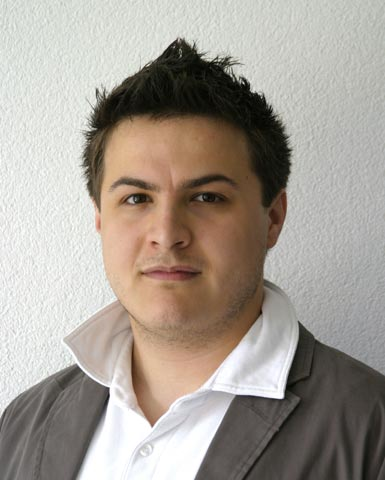
\includegraphics[width=3.8cm]{01_Introduction/media/photo_passeport_20.jpg}}\\
 	 
 	\vspace{0.5cm}

 	\textbf{Ingénierie d'application}  : Java, JR, Adobe AIR - FLEX, ActionScript, C, C++&&\\
 	\vspace{0.2cm}
 	\textbf{Développement Web} : PHP, HTML 4/5, CSS 2/3, Xataface, Contao, Joomla, Drupal, JSF / JSP, Adobe FLEX, ActionScript, Java EE&&\\
 	\vspace{0.2cm}
 	\textbf{Développement mobile} : IOS, Android&&\\
 	\vspace{0.2cm}
 	\textbf{Gestion des données} : MySQL, SQLite, Access, Oracle, SQLServer, technologies XML&&\\
\end{tabular}

\end{abstract}
	\pagebreak

	% begin header and footer for table of content
	\pagestyle{fancy}
	\renewcommand{\chaptermark}[1]{\markboth{#1}{}}
	\rhead{}
	
	\renewcommand{\thepage}{\roman{page}}
	
	\cleardoublepage
	\setcounter{page}{1}
	\tableofcontents
	\clearpage
	
	% begin header and footer for the rest of the document
	\makeatletter
	   \let\ps@plain\ps@fancy
	\makeatother
	\pagestyle{fancy}
	\renewcommand{\headrulewidth}{0.3pt}
	\renewcommand{\footrulewidth}{0.3pt}
	\renewcommand{\thepage}{\arabic{page}}
	
	
	\cleardoublepage
	\setcounter{page}{1}
	
	
	\lhead{\authornameone}
	\rhead{\today}
	\chead{\modulename}
	
	\lfoot{\subjectName}
	\rfoot{Page \thepage\ - \pageref{LastPage}}
	\cfoot{}
	%----------------------------------------------------------------------
	% contenu

	
%	%!TEX root = ../rapport.tex

\chapter{Introduction}
Ce chapitre introduit le rapport d'un projet de Bachelor de l'\emph{\gls{eiafr}} en filière informatique. Ce projet s'effectue à la fin des trois ans du cursus scolaire. Ci-dessous, en guise d'introduction, une description du contexte du projet a été repris de la donnée du projet ayant pour but d'expliquer dans les grandes lignes en quoi consiste le travail. Puis les objectifs et leurs tâches relatives sont posés. Pour terminer, vous pourrez trouver comment ce document est structuré.

\section{Contexte} % (fold)
\label{sec:contexte}
Ce projet de Bachelor est mon travail final d’étude à l'\emph{\gls{eiafr}} en section informatique. Ce dernier dure 7 semaines et est cloturé par une défense orale devant les superviseurs, le responsable ainsi que les experts.

\medskip

Vous trouverez ci-dessous l'énoncé original du projet tel qu'il a été présenté aux étudiants lors des choix.

\subsection{Enoncé original du projet} % (fold)
\label{sub:enonc_original_du_projet}
Ce projet porte sur la thématique du \emph{\gls{greecomputing}} 
(informatique écologique). Plus particulièrement, il s’inscrit dans le cadre du projet Hasler Green-Mod portant sur l’analyse de la consommation électrique des appareils ménagers d’un bâtiment en vue de faire de l’économie d’énergie.

\medskip

L'objectif du projet iGreenControl est d'analyser et développer une application \emph{\gls{ipad}} qui permette à des utilisateurs lambda de dessiner le plan de leur maison (ou de l'importer). Une fois que le plan sera acquis, il s’agira de positionner sur le plan les équipements électriques (prises électriques, appareils \emph{\gls{hifi}}, télévisions, ordinateurs, lampes et autres appareils 
ménagers).

\medskip

L'application tournera sur un équipement de type tablette \emph{\gls{ipad}}, Une attention particulière sera portée sur l’ergonomie de l'application. D'un point de vue architecture, le système s'articulera autour d'un serveur permettant la persistance du modèle de données ainsi que le contrôle des équipements. Les contraintes de ce serveur sont connues et un prototype existe déjà : système \emph{\gls{linux}}, base de données \emph{\gls{mysql}}, couche d’accès aux données sur protocole \emph{\gls{http}} avec échange d’informations \emph{\gls{xml}} ou \emph{\gls{json}}.
% subsection enonc_original_du_projet (end)
% section contexte (end)


\section{Objectifs} % (fold)
\label{sec:objectifs}
Cette section décrit les objectifs à atteindre à la fin du projet. Les objectifs secondaires seront réalisés uniquement si les primaires sont terminés et qu'il reste encore du temps au projet.

	\subsection{Primaires}

		\begin{itemize}
		
			\item Analyser et développer une application pour tablette \emph{\gls{ipad}} qui a comme but d'importer le plan d'une maison.
			\item Analyser et implémenter un serveur permettant la persistance du modèle de données.
			\item Permettre à l'utilisateur de positionner des zones sur le plan.
			\item Permettre à l'utilisateur de positionner des capteurs sur le plan et d'en modifier les paramètres.
		\end{itemize}


	\subsection{Secondaires}

		\begin{itemize}
		
			\item Analyser et développer une application pour tablette \emph{\gls{ipad}} qui a comme but de dessiner le plan d'une maison. L'utilisateur pourra également sauver et ouvrir ses plans.
			\item Permettre à l'utilisateur de positionner des actuateurs et de les utiliser.
		
		\end{itemize}
% section objectifs (end)

\section{Tâches} % (fold)
\label{sec:t_ches}
Cette section décrit les activités à effectuer pour atteindre les objectifs à la fin du projet. Les activités secondaires seront réalisées uniquement si les primaires sont terminées et qu'il reste encore du temps au projet.

	\subsection{Primaires}

		\begin{itemize}

			\item L'étude du langage, des concepts et de l'environnement de développement \emph{\gls{ios}}.
			\item L'analyse, la conception, l'implémentation et les tests de l'application pour la tablette iPad pour importer le plan d'une maison.
			\item L'étude et l'analyse des technologies \emph{\gls{http}}, \emph{\gls{json}}, des principes \emph{\gls{rest}} ou \emph{\gls{rest}}ful, \emph{\gls{jaxrs}}, \emph{\gls{jpa}} de la plateforme actuelle.
			\item La modification de la plateforme actuelle pour implémenter les besoins.
			\item L'analyse, la conception, l'implémentation et les tests de l'application pour pouvoir positionner des zones ainsi que des capteurs sur le plan et modifier les paramètres de ces derniers.
		\end{itemize}


	\subsection{Secondaires}

		\begin{itemize}
			\item L'analyse, la conception, l'implémentation et les tests de l'application pour dessiner le plan d'une maison ainsi que pour sauver et ouvrir les plans.
			\item L'analyse, la conception, l'implémentation et les tests de l'application pour pouvoir positionner des actuateurs sur le plan et les utiliser.
		\end{itemize}
% section t_ches (end)

\section{Structure du document} % (fold)
\label{sec:structure_du_document}

Le deuxième chapitre explique l'organisation qui a été tenue tout au long du projet en faisait référence à la planification et aux séances de projet effectueé.

\medskip

Le troisième chapitre a pour but d'aider au maximum la prise en main de travaux futurs sur le projet puisqu'il cite les outils qui ont été employés pour mener à bien le travail.

\medskip

Avec le quatrième chapitre, nous entrons dans le vif du sujet puisqu'il explique les principes, les objectifs et des exemples du \emph{\gls{greecomputing}} à l'heure d'aujourd'hui.

\medskip

Dans le cinquième chapitre, il a été question de faire une analyse de l'application dans sa globalité afin d'entrer dans le projet avec le plus d'informations possibles et répondre aux questions qui restent floues au début du projet. 

\medskip

Le sixième chapitre découle de la conception effectuée pour l'application générale. Cela permet de mieux illustrer les besoins et les objectifs du projet.

\medskip

Le septième chapitre concerne la partie cliente du système. Il s'agit de l'application \emph{\gls{ipad}}. La structure de ce chapitre suit un déroulement assez habituel de développement de logiciel puisqu'il a été découpé en une partie d'analyse, de conception, de réalisation et de tests.

\medskip

Le huitième chapitre comporte la même structure que le septième mais pour la partie serveur du système. Il s'agit donc du \emph{\gls{webservice}} qui sera utilisé par le client.

\medskip 

Dans le chapitre suivant, le neuvième, les tests qui ont été effectués sur l'ensemble du projet ont été reportés.

\medskip

L'avant dernier chapitre, le dixième, intitulé \emph{Résultats}, a pour but d'illustrer par des captures d'écrans les résultats finaux obtenus. Ce chapitre est également un guide pour tous les utilisateurs qui veulent employer l'application.

\medskip

Ce rapport se terminera par une conclusion mettant en avant un bilan, mes impressions personnelles, les problèmes rencontrés ainsi que les améliorations qui peuvent être effectuées.

\medskip

Vous pourrez trouver en annexe le planning effectué au début du projet et la description de la structure du \emph{\gls{dvd}} qui se trouve collé à la fin de ce rapport.

% section structure_du_document (end)
%	%!TEX root = ../rapport.tex

\chapter{Organisation} % (fold)
\label{cha:organisation}

Ce chapitre explique l'organisation qui a été tenue tout au long du projet. 

\section{Planification} % (fold)
\label{sec:planification}
La planification est disponible en annexe \ref{cha:annexe:planning}. 

\medskip

Comme la taille du document a du être diminuée pour avoir sa place dans ce rapport, il est possible de trouver le planning au format informatique disponible à l'adresse \cite{online:forge:planfin}.

\medskip

La planification a été découpée en 7 semaines et comporte, dans les grandes lignes, les tâches qui devront être effectuées.

\medskip

Les carrés bleus représentent le temps prévu pour la tâche et les verts sont le temps effectué réellement. Il est ainsi possible de voir par exemple si l'on est trop optimiste ou au contraire trop pessimiste lorsqu'on prévoit des durées pour un projet.

\subsection{Dates clefs} % (fold)
\begin{table}[h] % dates clefs
\begin{tabularx}{\textwidth}{|X|X|X|}
  \hline
  \bf{Activité} & \bf{Jour} & \bf{Heure} \\  \hline
  Début du projet &	Mardi 29.05.2012 & -\\  \hline
Rendu des rapports et du flyer au responsable
de filière	& Vendredi 13.07.2012 &	17:00 \\  \hline
Poster &	Jeudi	06.09.2012 &	12:00 \\  \hline
Présentation des travaux de Bachelor &	Vendredi 07.09.2012 \newline
Samedi	
08.09.2012 &	-\\  \hline
Défense orale &	Lundi 10.09.2012 \newline
Mardi 11.09.2012\newline
Mercredi 12.09.2012 &-\\  \hline
\end{tabularx}
\caption{Tableau récapitualif des dates clefs}
\end{table}
% subsection dates_clefs (end)
% subsection subsection_name (end)
% section planification (end)

\section{Séances} % (fold)
\label{sec:s_ances}
Des séances avec les superviseurs ont été tenues chaque semaine pour expliquer les principales tâches effectuées et ainsi montrer l'avancement du projet. Ces séances permettaient de poser des questions et de recevoir, avec plaisir, des conseils et des feedbacks sur le travail.
% section s_ances (end)

% chapter organisation (end)


\chapter{Environnement de travail} % (fold)
\label{cha:environnement_de_travail}

Le but de ce chapitre est de faciliter la prise en main future du projet par une autre personne. En effet, je reporte ici tous les outils et les appareils que j'ai utilisés pour mener à bien ce projet. Vous trouverez dans ce chapitre également les liens vers les différents documents qui ont été créés durant le travail.

\section{Outils de travail} % (fold)
\label{sec:outils_de_travail}

\subsection{Ordinateur} % (fold)
\label{sub:macbook_pro}
La totalité des activités a été effectuée sur un ordinateur portable d'Apple.

\begin{description}
	\item[Version] MacBook Pro 13 pouces, début 2011
	\item [Système d'exploitation] Mac OS X Lion 10.7.4 
\end{description}
% subsection macbook_pro (end)

\subsection{Tablette} % (fold)
\label{sub:tablette}
L'application tournera sur une tablette de type iPad conçue et développée par Apple.

\begin{description}
	\item[Modèle] iPad 2
	\item [Système d’exploitation] iOS 5.1.1
	\item [Résolution] 1024 x 768 
\end{description}
% subsection tablette (end)

\subsection{Programmes} % (fold)
\label{sub:programmes}
J'énumère ci-dessous les programmes que j'ai utilisés tout au long du projet. Ces programmes sont des versions pour Mac OSX.

\medskip

\begin{itemize}
	\item Sublime Text 2 et TeXLive-2011 pour l'édition du rapport
	\item Visual Paradigm et OmniGraffle version 5.3.6 pour les diagrammes de conception
	\item XCode version 4.3.2 pour la réalisation du client
	\item Eclipse version 3.7.2 pour la réalisation du webservice
	\item WizTools.org RESTClient version 2.4 pour envoyer des requêtes \emph{\gls{rest}} sur un \emph{\gls{webservice}}
	\item MySQL Workbench version 5.2 pour la gestion de la base de données
\end{itemize}
% subsection programmes (end)



% section outils_de_travail (end)

\section{Partage de documents} % (fold)
\label{sec:partage_de_documents}
% section partage_de_documents (end)

Pour partager les documents pendant le projet, j'ai utilisé la \emph{\gls{forge}} mise à disposition par l'\emph{\gls{eiafr}} et disponible à l'adresse \cite{online:forge}.

\medskip

\begin{itemize}
	\item Les versions de la \textbf{planification} sont disponibles à l'adresse \cite{online:forge:plan}
	\item Les versions du \textbf{cahier des charges} sont disponibles à l'adresse \cite{online:forge:spec}
	\item Les \textbf{procès-verbaux} sont disponibles à l'adresse \cite{online:forge:pv}
	\item Ce présent \textbf{rapport} est disponible à l'adresse \cite{online:forge:rapport}. Celui-ci est en deux versions. En effet, il existe une version qui est destinée à être imprimée et une autre destinée à être lue sur un ordinateur. Ceci a été fait dans le but d'avoir un rapport agréable à lire dans les deux cas.
	\item Le \textbf{journal de bord} est disponible à l'adresse \cite{online:forge:wiki}.
\end{itemize}

% chapter environnement_de_travail (end)
%
%	%!TEX root = ../rapport.tex

\chapter{Green Computing}

Ce chapitre a comme objectif d'éclaircir le sujet en définissant de quoi il parle et également de citer quelques concepts de l'\emph{informatique verte}.
\section{Définition} % (fold)
\label{sec:d_finition}
\begin{shadequote}
L'expression anglophone « Green computing » (ou encore « green information technology », en abrégé « green IT ») signifie en français mot à mot « informatique verte », plus largement « informatique éco-responsable ». Le concept désigne un état de l'art informatique qui vise à réduire l'empreinte écologique, économique, et sociale des technologies de l'information et de la communication (TIC). Il s'agit d'une manière globale et cohérente de réduire les nuisances rencontrées dans le domaine des équipements informatiques et ce, « du berceau jusqu'à la tombe » de chaque équipement : soit aux différents stades de fabrication, d'utilisation (consommation d'énergie) et de fin de vie (gestion/récupération des déchets, pollution, épuisement des ressources non renouvelables). \par\emph{Définition tirée de Wikipedia, disponible sur le site \cite{online:wiki:green}}
\end{shadequote}

L'\emph{informatique verte} ou le \emph{Green Computing} ou encore le \emph{Green IT} est un concept visant à réduire la mauvais impact de l'informatique et la télécomunnication sur l'environnement.

\medskip

La définition est tout de fois élargie dans certains cas. Effectivement, on parle également de \emph{Green Computing} dans les cas où, par exemple, des applications sont conçues et développées dans un but écologique. Typiquement, une application qui a pour but de récolter des informations de consommation énergique et d'en faire des graphiques pour les exposer à des personnes peut faire partie du concept de l'\emph{informatique verte}.

\medskip

Ci-dessous, des exemples de concepts faciles à mettre en place et qui font déjà en sorte de rendre le tout \emph{Green} !
% section d_finition (end)


\section{Exemple pour un parc informatique} % (fold)
\label{sec:exemple_pour_un_parc_informatique}

Bien qu'un parc informatique puisse ne pas être \emph{Green}, il est tout à fait possible de le rendre de la sorte.

\medskip

\begin{itemize}
	\item Virtualiser des serveurs et des ordinateurs afin de réduire la consommation électrique. En effet, il est possible de nos jours de rendre virtuelles des machines et ainsi en faire tourner plus d'une sur une seule machine physique.
	\item Supprimer les échanges papier et utiliser les courriers électroniques afin d'économiser le papier
\end{itemize}

\section{Ma contribution pendant le projet} % (fold)
\label{sec:ma_contribution_pendant_le_projet}

Pendant le projet, j'ai essayé de rendre mon train de vie autant écologique que possible ! Je pense que ces petites astuces ont contribué, même si ce n'est qu'un tout petit peu, à l'écologie et au \emph{Green Computing}.

\medskip

\begin{itemize}
	\item Prendre les transports publics pour les longs trajets
	\item Faire les courts trajets à pieds plutôt qu'en véhicule
	\item Eviter d'imprimer beaucoup de documents  et plutôt utiliser les formats électroniques 
	\item Utiliser un ordinateur conçu pour avoir le moins d'impact possible sur l'environnement
\end{itemize}

\begin{shadequote}
MacBook Pro is designed with the following features to reduce environmental impact. \par\emph{Citation tirée du site \cite{online:apple:green}}
\end{shadequote}
% section ma_contribution_pendant_le_projet (end)


% section exemple_pour_un_parc_informatique (end)
%
%	%!TEX root = ../rapport.tex

\chapter{Analyse de l'application générale}
Le but de ce chapitre est de décrire l'analyse qui a été faite au début du projet afin de faciliter le déroulement des étapes suivantes comme la conception, l'implémentation et les tests du système.

\medskip

Cette partie décrit l'analyse du projet en général. L'analyse plus spécifique de la partie \emph{client} et \emph{serveur} se fait, respectivement, dans la section \ref{sec:analyse_client} et \ref{sec:analyse_serveur}.

\section{Base de données} % (fold)
\label{sec:base_de_donn_es}
La base de données pour le projet existe déjà. Néanmoins, il n'est pas impossible qu'il y aura des changements à effectuer pour répondre correctement aux besoins de l'application. Cette base de données résulte de modifications et d'ajouts sur celle utilisée pour le projet Watt-ICT. En effet, l'\gls{eiafr} a repensé certains points du modèle de données afin de partir avec une meilleure base.

\medskip

La figure \ref{gra:bddv2} est le résultat du travail sur la base de données avant le projet.

\medskip

En analysant la base de données, nous pouvons nous apercevoir des faits suivants : 

\medskip

\begin{itemize}
    \item Un utilisateur peut avoir une, plusieurs ou aucune maisons
    \item Les maisons peuvent être reliées à plusieurs utilisateurs
    \item Une zone ne peut être reliée qu'à une seule maison
    \item Une zone peut être reliée à plusieurs capteurs
    \item Un capteur ne peut être relié qu'à une seule zone
    \item Les capteurs sont reliés à des données capturées et il existe une table qui permet de récuperer les dernières données du capteur
    \item Chaque donnée est reliée à un autre type avec lequel on peut récupérer le nom, l'unité, etc...
    \item On peut déjà voir qu'il y aura des champs à ajouter concernant l'image du plan
    \item Il faudra également ajouter des positions pour le plan, une largeur, une hauteur
    \item Même constatation pour les zones puisqu'il faudra savoir où elles doivent être placées, la largeur et la hauteur
\end{itemize}


\begin{figure}[H]
    	\centering
    	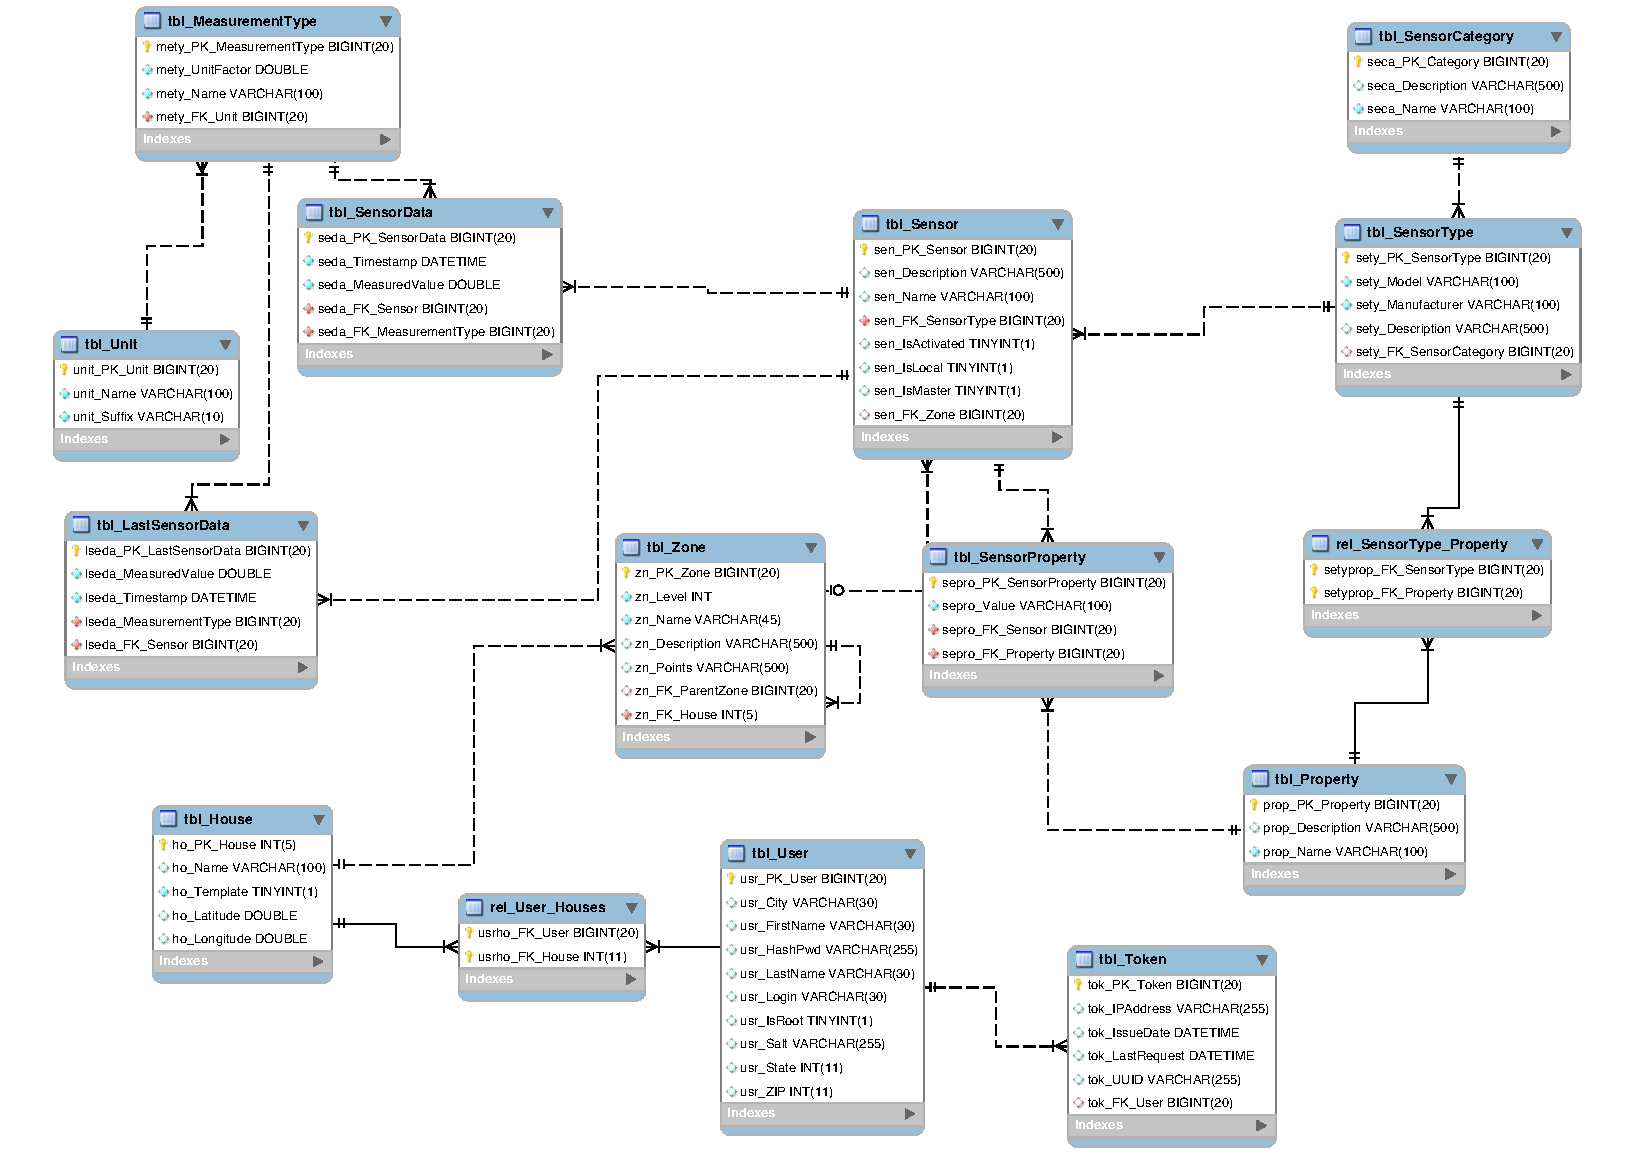
\includegraphics[width=\textwidth]{00_media/03_bddV2.pdf}
    	\caption{Base de données avant le projet}
    	\label{gra:bddv2}
\end{figure}
% section base_de_donn_es (end)


\section{Prise en main de Watt-ICT} % (fold)
\label{sub:etat_actuel_du_syst_me}
Il existe actuellement une plateforme qui permet de gérer des capteurs dans différentes maisons. Cette application permet en effet d'ajouter des maisons pour ensuite les lister avec leurs capteurs associés. De plus, elle permet d'avoir des informations sur la fréquence, la puissance, etc.. Ce projet a donc un but écologique puisqu'il permet de récupérer des données intéressantes en vue de faire de l'économie d'énergie.

\medskip

Malheureusement, cette plateforme comporte certains bugs, n'est pas des plus conviviales à utiliser et ne présente aucune documentation. De plus, les personnes travaillant à l'EIA-FR trouvent que la base de données n'est pas très bien pensée et c'est pour cette raison qu'ils l'ont redesignée pour des projets à l'école.

\medskip

Il faudra donc reprendre les meilleures parties, les adapter et implémenter les éléments indispensables au bon fonctionnement du projet.

\medskip

Cette section décrit les étapes qui ont été nécessaires afin de pouvoir démarrer la plateforme \emph{Watt-ICT}. Les deux étapes principales sont la mise en place de la base de données et la configuration d'\emph{\gls{eclipse}}
\subsection{Mise en place de la base de données} % (fold)
\label{sub:mise_en_place_de_la_base_de_donn_es}
Le plateforme nécessite la mise en place d'une base de données pour pouvoir récupérer les informations. Pour se faire, j'ai utilisé \emph{\gls{mamp}} dans sa version 2.0.5.

\medskip

Pour mettre en place la base, j'ai utilisé le fichier \emph{\gls{sql}} disponible sur la Forge à l'adresse \url{https://forge.tic.eia-fr.ch/attachments/download/2910/dump.sql}. J'ai simplement utilisé la fonction qui permet d'importer un fichier contenant du code \emph{\gls{sql}}.

\medskip

Voici les informations nécessaires pour la suite:

\medskip

\begin{itemize}
 	\item Hôte : {\bf localhost}
 	\item Port : {\bf 8889}
 	\item Utilisateur : {\bf root}
 	\item Mot de passe : {\bf root}
 	\item Nom de la base : {\bf green-app}
 \end{itemize} 
% subsection mise_en_place_de_la_base_de_donn_es (end)

\subsection{Configuration d'Eclipse} % (fold)
\label{sub:eclipse}

% subsection eclipse (end)
Afin de lancer le programme Watt-ICT, il a été nécessaire d'effectuer plusieurs opérations. Pour commencer, j'ai utilisé \emph{\gls{eclipse}} dans sa version 3.7.2. Voici la marche à suivre qui a été suivie afin de pouvoir accéder à la plateforme.

\medskip

Pour commencer, afin de pouvoir importer un projet \emph{\gls{maven}}, il faut,  dans \emph{\gls{eclipse}}, installer les plugins suivants à l'aide du menu \emph{Help} en cliquant sur \emph{Install New Software} :

\medskip

\begin{itemize}
    \item \emph{Subversive Site} disponible grâce à l'adresse \cite{online:eclipse:subversive}
    \item \emph{Maven Integration for Subclipse} disponible grâce à l'adresse \cite{online:eclipse:mavensubclipse}
    \item \emph{Maven SCM Handler for Subversive} disponible grâce à l'adresse \cite{online:eclipse:scm}
\end{itemize}

\medskip

Une fois ceci fait, il est possible de créer un nouveau projet \emph{\gls{maven}} en faisant un \emph{Checkout} comme le montre la figure \ref{gra:mavenProjectCheckout}.

\begin{figure}[H]
    	\centering
    	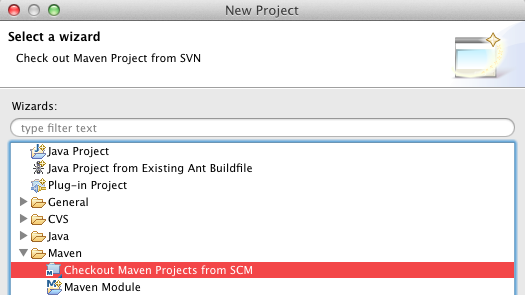
\includegraphics[width=300px]{00_media/02_mavenProjet.png}
    	\caption{Création d'un nouveau projet Maven}
    	\label{gra:mavenProjectCheckout}
\end{figure}

Il faut ensuite sélectionner le type d'url \emph{(svn)} et entrer son adresse qui est \url{https://forge.tic.eia-fr.ch/svn/eiafr/tic/acad/info/1112/igreencontrol/trunk}. On peut désormais directement cliquer sur \emph{Finish}.

\medskip

Lorsque ceci est fait, un nouveau projet apparaît. Il faut encore éditer le fichier de configuration pour accéder à la base de données qui a été mise en place précédemment. Ce fichier se nomme \emph{ga-service.conf} et le code \ref{lst:bddConfig} montre le contenu qui a été inséré.

\begin{lstlisting}[language={XML}, caption={Fichier de configuration BDD}, label={lst:bddConfig}]
# Database access parameters
db.url = jdbc:mysql://localhost:8889/green-app
db.user = root
db.password = root

# HTTP parameters
http.url = localhost/ga-service
http.port = 9998
\end{lstlisting}

Il est maintenant possible d'accéder à la plateforme via l'adresse \url{http://localhost:9998/ga-service/index.html}
% section etat_actuel_du_syst_me (end)

%	%!TEX root = ../rapport.tex
\chapter{Conception de l'application générale}
Dans ce chapitre, la conception de l'application générale est exposée. Celle-ci n'est pas des plus détaillée car une conception plus spécifique du client et du serveur se feront respectivement dans les parties \ref{section:conception_client} et \ref{section:conception_serveur}.

\section{Diagramme de cas d'utilisation} % (fold)
\label{sec:diagramme_de_cas_d_utilisation}

La première étape de cette conception a été d'exprimer, simplement, ce qui sera possible de faire dans l'application et d'avoir une base pour en discuter avec un client. Pour se faire, un diagramme des cas d'utilisation a été dessiné et est représenté par la figure \ref{gra:usecase}. Par la suite, une explication des différents éléments importants à la compréhension de ce diagramme est présentée.

\begin{figure}[H]
    	\centering
    	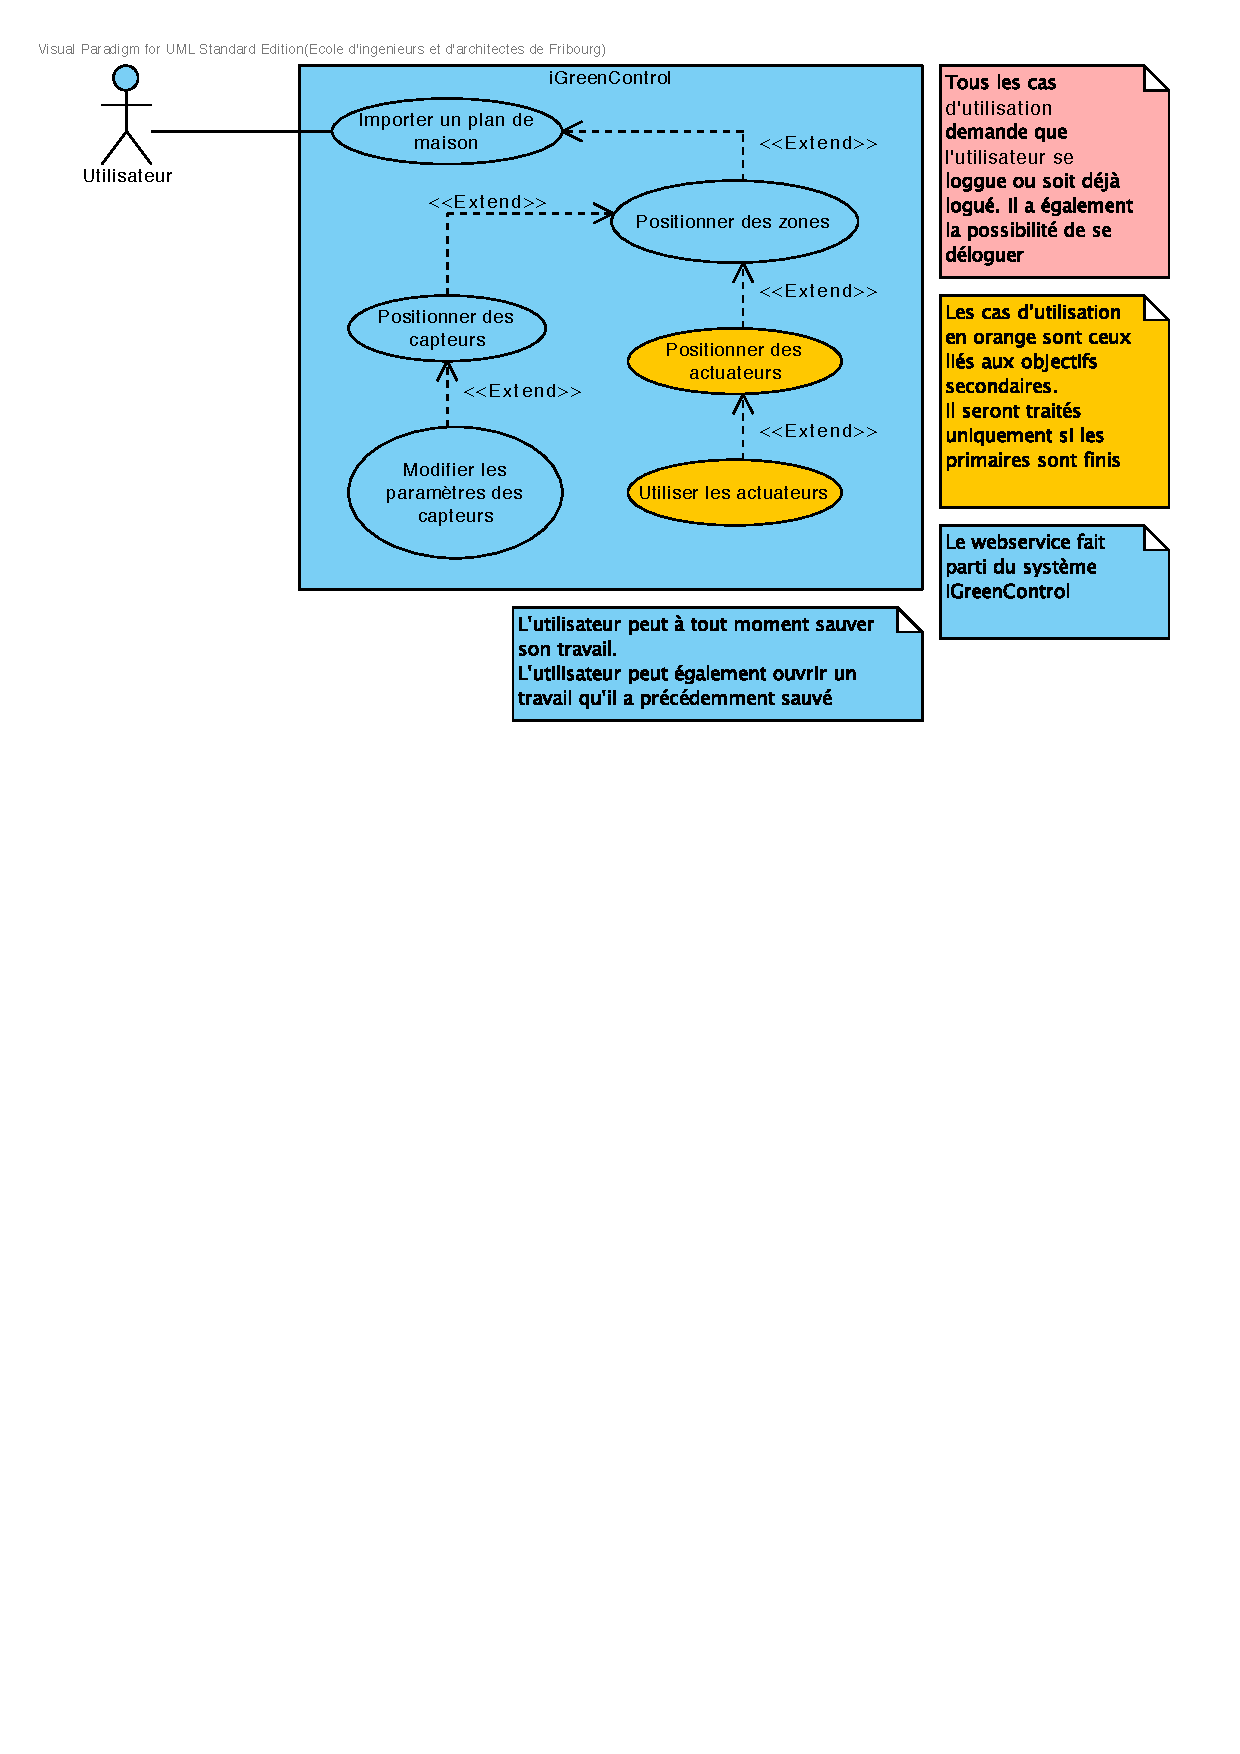
\includegraphics[width=\textwidth]{00_media/04_diagramme_usecase.pdf}
    	\caption{Diagramme de cas d'utilisation du système iGreenControl}
    	\label{gra:usecase}
\end{figure}


\subsection{Les cas d'utilisation} % (fold)

Ci-dessous une explication des différents cas d'utilisation. Ces explications sont brèves car elles seront repris plus en détails dans la partie \ref{section:conception_client}.

\medskip

\begin{itemize}
	\item \textbf{Importer un  plan de maison} consiste à permettre à l'utilisateur final de choisir par exemple une photo dans la librairie des photos et de l'importer dans l'application. 
	\item \textbf{Positionner des zones} demande que l'utilisateur ait importé un plan. Il peut ainsi disposer différentes zones sur ce plan.
	\item \textbf{Positionner des capteurs} demande que l'utilisateur ait positionné des zones sur le plan. Il peut ainsi insérer des capteurs.
	\item \textbf{Modifier les paramètres des capteurs} demande que l'utilisateur ait positionné des capteurs dans des zones. Il peut ainsi en modifier différentes paramètres (nom, catégorie, ...)
	\item \textbf{Positionner des actuateurs} demande que l'utilisateur ait positionné des zones sur le plan. Il peut ainsi insérer des actuateurs. Ceci est un cas d'utilisation issu d'un objectif secondaire.
	\item \textbf{Utiliser les actuateurs} demande que l'utilisateur ait inséré des actuateurs dans des zones. Il peut ainsi utiliser les actuateurs. Ceci est un cas d'utilisation issu d'un objectif secondaire.
\end{itemize}

\subsection{Utilisateur}

L'acteur principal de ce système est l'utilisateur final qui se servira de l'\emph{\gls{ipad}} pour utiliser l'application \emph{iGreenControl}.

\subsection{Authentification}
Sur le diagramme, le fait de devoir s'identifier à l'aide d'un nom d'utilisateur et d'un mot de passe n'a pas été reporté en tant que cas d'utilisation mais en tant que note. Cela a été fait pour alléger le diagramme. 

\begin{shadequote}
Tous les cas d'utilisation demande que l'utilisateur se loggue ou soit déjà logué. Il a également la possibilité de se déloguer. \par\emph{Note du cas d'utilisation}
\end{shadequote}

\subsection{Ouverture et sauvegarde}
Sur le diagramme, le fait de pouvoir sauvegarder et ouvrir un travail n'est pas représenter et est introduit par une note. Cela a été fait pour alléger le diagramme.

\begin{shadequote}
L'utilisateur peut à tout moment sauver son travail.
L'utilisateur peut également ouvrir un travail qu'il a précédemment sauvé. \par\emph{Note du cas d'utilisation}
\end{shadequote}


\subsection{Webservice}

Le tout s'articulera autour d'un \emph{\gls{webservice}} qui permettra de demander et d'envoyer des informations dans la base de données. Comme ce service fait parti du système, il  n'est pas représenté par un acteur mais est bel et bien dans le système \emph{iGreenControl}.

\begin{shadequote}
Le \emph{\gls{webservice}} fait parti du système iGreenControl. \par\emph{Note du cas d'utilisation}
\end{shadequote}


\subsection{Objectifs primaires et secondaires}
Le diagramme différencie les objectifs primaires des objectifs secondaires.

\begin{shadequote}
Les cas d'utilisation en orange sont ceux liés aux objectifs secondaires.
Il seront traités uniquement si les primaires sont finis. \par\emph{Note du cas d'utilisation}
\end{shadequote}

% subsection explications (end)

% section diagramme_de_cas_d_utilisation (end)
\section{Scénario générale de l'application} % (fold)
\label{sub:concept_de_l_application}
L'utilisateur importe une photo du plan de sa maison ou son appartement. 

\medskip

Il peut ensuite créer des zones par pièce (ex: une chambre = une zone). Les pièces du même type peuvent être regroupées dans une zone (ex: toutes les chambres = une zone "mère").

\medskip

Lorsque ceci est fait, il a la possibilité de positionner des capteurs dans les différentes zones et gérer les paramètres généraux de ceux-ci.

\medskip

Enfin, les données récupérées pourront être exploitées par d'autres personnes en vue de faire de l'économie d'énergie. Ce projet a donc un principe d'informatique écologique. 

\medskip

Optionnellement, des actuateurs pourront être placés dans des zones dans le but par exemple d'éteindre ou d'allumer une lampe.

% section concept_de_l_application (end)

\section{Architecture générale de l'application} % (fold)
\label{sub:architecture_g_n_rale_de_l_application}
La figure \ref{gra:archiGenerale} représente l'architecture générale de l'application.
\begin{figure}[H]
    	\centering
    	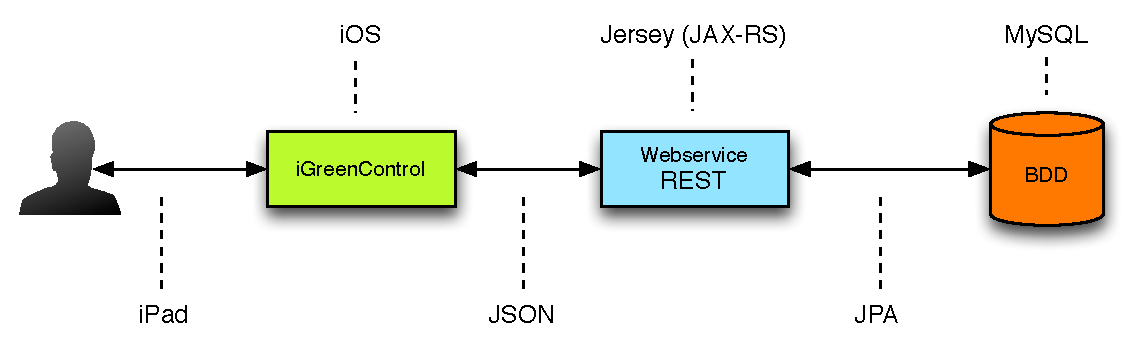
\includegraphics[width=\textwidth]{00_media/02_archi.pdf}
    	\caption{Architecture générale de l'application}
    	\label{gra:archiGenerale}
\end{figure}
% section architecture_g_n_rale_de_l_application (end)


L'utilisateur, muni d'un \emph{\gls{ipad}}, utilise l'application \emph{iGreenControl} qui tourne sur \emph{\gls{ios}}.

\medskip

L'application récupère les données dont elle a besoin sous format \emph{\gls{json}} depuis un \emph{\gls{webservice}}.

\medskip

Le \emph{\gls{webservice}} est de type \emph{\gls{rest}} et implémente \emph{\gls{jaxrs}} qui est une interface de programmation \emph{\gls{java}} qui permet de créer des \emph{\glspl{webservice}}. J'utiliserai \emph{Jersey} qui est une des références en implémentation de \emph{\gls{jaxrs}}.

\medskip

Le \emph{\gls{webservice}} travaille avec une base de données de type \emph{\gls{mysql}} via \emph{\gls{jpa}} qui est une interface de programmation qui permet d'organiser nos données relationnelles avec \emph{\gls{java}}.

\section{Base de données} % (fold)
\label{sec:base_de_donn_es}
Pour ce qui est de la base de données, il n'y a pas eu de grands changements pour le projet si ce n'est ajouter des informations pour retenir :

\medskip

\begin{itemize}
    \item L'image du plan
    \item La position en x et en y du plan
    \item La largeur et la longueur du plan
    \item La position en x et en y d'une zone
    \item La largeur et la longueur d'une zone
    \item La valeur total des rotations effectuée sur une zone
\end{itemize}

\medskip

Le tout a été ajouté sous forme de chaîne de caractères.
% section base_de_donn_es (end)

%
%	%!TEX root = ../rapport.tex
\chapter{Analyse, conception, réalisation et tests de la partie cliente}
\label{cha:analyse_client}

Ce chapitre regroupe les différentes parties qui ont été effectuées pour la partie cliente du système. Il s'agit donc de l'application \emph{\gls{ipad}} qui sera analysée. Ensuite une conception plus détaillée sera faite d'une part pour mieux se faire comprendre par le client et d'une autre part pour faciliter la partie suivante qui est la réalisation. Pour terminer ce chapitre, les résultats des tests effectués sur le client seront reportés.

\section{Analyse} % (fold)
\label{sec:analyse_client}
Vous trouverez ci-dessous l'analyse qui a été faite sur le développement \emph{\gls{ios}} ou sur le principe du format \emph{\gls{json}}. D'autres points ont été analysés afin de se faire une première idée sur les possibilités qui s'offriront pour le développement.
\subsection{Concepts de développement sur iOS} % (fold)
\label{sub:concepts_de_d_veloppement_sur_ios}

\subsubsection{Protocoles \& Delegates}
Les \emph{protocoles} et les \emph{delegates} sont intimement liés lorsqu'on développe en \emph{\gls{obj-c}}.

\medskip 

Un protocole permet de déclarer des méthodes qui peuvent être implémentées par une classe. Cela ressemble fortement aux interfaces dans le monde \emph{\gls{java}}. Le code \ref{lst:protocol} montre comment déclarer un protocole alors que le code \ref{lst:protocol2} comment suivre ce protocole. On dit que la classe qui suit un protocole est son délégué.

\begin{lstlisting}[language={C}, caption={Déclarer un protocole Printing}, label={lst:protocol}]
@protocol Printing
	-(void) print;
@end
\end{lstlisting}

\begin{lstlisting}[language={C}, caption={Suivre le protocole Printing}, label={lst:protocol2}]
#import <Foundation/NSObject.h>
#import "Printing.h"

@interface Fraction: NSObject <Printing> {
    int numerator;
    int denominator;
}
\end{lstlisting}
\subsubsection{Storyboard}
\emph{Storyboard} est une nouvelle manière de dessiner ou designer les interfaces que l'on crée dans \emph{\gls{xcode}}. 

\medskip

Cela permet également, et c'est là un point très fort, de définir les différentes interactions qui existent entre les interfaces de notre application. La figure \ref{gra:storyboard} montre un exemple de storyboard tiré du site internet \cite{online:RayWenderlich}.

\begin{figure}[H]
    	\centering
    	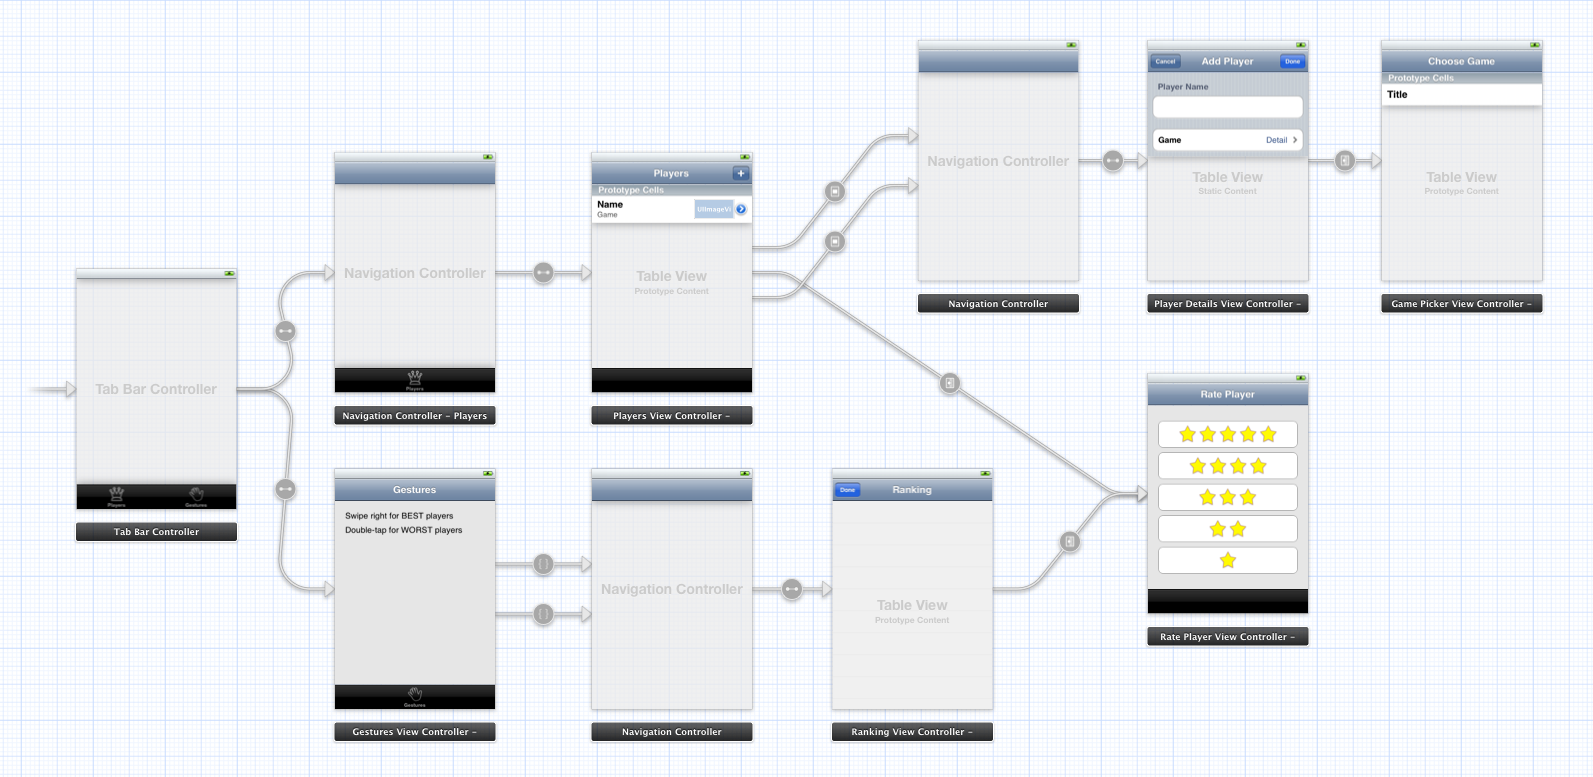
\includegraphics[width=\textwidth]{00_media/storyboard.png}
    	\caption{Exemple de Storyboard tiré du site \cite{online:RayWenderlich}}
    	\label{gra:storyboard}
\end{figure}
% subsection concepts_de_d_veloppement_sur_ios (end)

\subsubsection{ARC}
Depuis \emph{\gls{ios}} 5, \emph{\gls{arc}} permet de ne plus nous soucier des références en effectuant des \emph{retain} ou des \emph{release}.

\medskip

Ce n'est pas exactement un \emph{Garbage collector} \emph{(Ramasseur de miettes)} qui est par exemple effectué pour du \emph{\gls{java}}. En effet, les \emph{retain} ou les \emph{release} que l'on insérait avant sont simplement ajoutés automatiquement. 

\medskip

C'est pour cette raison qu'il est d'ailleurs toujours obligatoire, comme le montre le code \ref{lst:arc} tiré d'un exemple sur le site \cite{online:LongWeekendLLC}, de créer un \emph{Pool Auto Release} dans le \emph{Main} d'un programme lorsqu'on crée une application.
\begin{lstlisting}[language={C}, caption={Autorelease Pool tiré d'un exemple du site \cite{online:LongWeekendLLC}}, label={lst:arc}]
int main(int argc, char *argv[])
{
  @autoreleasepool {
    return UIApplicationMain(argc, argv, nil, NSStringFromClass([ExampleAppDelegate class]));
  }
}
\end{lstlisting}

\subsubsection{Gestures recognizers}

Les reconnaissances de gestes sur une \texttt{UIView} ou une de ses sous-classes sont disponibles depuis la version 3.2 \emph{\gls{ios}}. La liste ci-dessous décrit chaque \emph{Gesture Recognizer}.

\bigskip

\begin{itemize}
  \item \texttt{UITapGestureRecognizer} permet de détecter 1 ou plusieurs tapes sur l'écran. On peut définir le nombre de tapes requises.
  \item \texttt{UIPinchGestureRecognizer} permet de détecter lorsque 2 doigts vont dans le sens contraire comme par exemple pour agrandir un objet.
  \item \texttt{UIRotationGestureRecognizer} permet de détecter lorsque 2 doigts sont opposés et font un mouvement circulaire comme par exemple changer la rotation d'une forme.
  \item \texttt{UISwipeGestureRecognizer} permet de détecter une glissement avec un ou plusieurs doigts sur un objet dans une direction qui est définit par nos propres soins.
  \item \texttt{UIPanGestureRecognizer} permet de détecter lorsqu'un utilisateur a cliqué sur un objet et désire le déplacer. On peut également définir le nombre de doigts.
  \item \texttt{UILongPressGestureRecognizer} permet de détecter lorsqu'un utilisateur clique une certaine durée sur un objet. Cette durée peut être définie.
\end{itemize}

\bigskip

Il est possible d'ajouter une reconnaissance de geste sur une \texttt{UIView} grâce à la méthode \texttt{addGestureRecognizer:}. 

\medskip

Le code \ref{lst:grexemple} en donne un exemple. En effet, on ajoute un \texttt{UITapGestureRecognizer} sur la vue principale ce qui aura comme conséquence d'appeler la méthode \texttt{tapOnScreen:} lorsque l'utilisateur aura tapé 2 fois sur l'écran.

\begin{lstlisting}[language={JAVA}, caption={Exemple d'ajout gesture recognizer}, label={lst:grexemple}]
UITapGestureRecognizer *tapView = [[UITapGestureRecognizer alloc] initWithTarget:self action:@selector(tapOnScreen:)];
tapView.numberOfTapsRequired = 2;
[self.view addGestureRecognizer:tapView];
\end{lstlisting}

Le code \ref{lst:tapOnScreen} montre comment déclarer les méthodes qui traîte les reconnaissances de gestes.

\begin{lstlisting}[language={JAVA}, caption={Exemple de traitement d'un geste}, label={lst:tapOnScreen}]
- (void)tapOnScreen:(UITapGestureRecognizer*)gesture {
    NSLog(@"Tap on the screen");
}
\end{lstlisting}

Il est également possible de spécifier si la reconnaissance doit être détectée ou non grâce à la méthode du \emph{delegate} de \emph{UIGestureRecognizerDelegate} reportée au code \ref{lst:shouldReceiveTouch}. Cette méthode retourne alors un \emph{BOOL}.
\begin{lstlisting}[language={JAVA}, caption={Gesture shouldReceiveTouch}, label={lst:shouldReceiveTouch}]
- (BOOL)gestureRecognizer:(UIGestureRecognizer *)gestureRecognizer shouldReceiveTouch:(UITouch *)touch;
\end{lstlisting}

\subsection{Utilisation des ressources sur l'iPad} % (fold)
\label{sub:utiliser_des_ressources_de_l_ipad}
Lorsque l'utilisateur veut importer une photo d'un plan dans l'application, il faut que cela se fasse facilement. Il y a plusieurs moyens de le faire. Voici une liste qui regroupe des idées pour cette partie : 

\medskip

\begin{itemize}
	\item Sélectionner une photo dans la librairie de photos sur l'\emph{\gls{ipad}}
	\item Sélectionner une photo sur un disque qui permet de partager (DropBox, Wuala, ...)
	\item Prendre directement une photo depuis l'application
\end{itemize}

\medskip

Une analyse des différentes possibilités a été faite, ci-dessous, afin d'avoir déjà une idée sur la complexité de mise en place et le niveau de difficulté de son intégration dans une application \emph{\gls{ipad}}.

\subsubsection{Photos Library}
\emph{\gls{ios}} propose dans sa couche \emph{UIKit} une classe \emph{UIImagePickerController} afin de permettre à l'utilisateur de choisir une photo ou une vidéo sauvée sur des appareils tels que l'iPhone, l'iPod ou l'\emph{\gls{ipad}} par exemple. Grâce à cette classe, on peut faire en sorte de proposer directement de prendre une photo ou une vidéo. Une documentation est disponible sur le site \cite{online:iosimagepickercontroller}.

\medskip

Pour utiliser cela, il faut suivre le protocole \emph{UIImagePickerControllerDelegate} qui propose deux méthodes : 

\begin{description}
  \item [imagePickerController:didFinishPickingMediaWithInfo:] est appelée lorsque l'utilisateur a choisi une image ou une vidéo.
  \item [imagePickerControllerDidCancel:] est appelée lorsque l'utilisateur décide de ne pas choisir d'image en quittant l'interface.
\end{description}

\medskip

Une documentation est disponible sur le site \cite{online:iosimagepickerdelegate}.


\subsubsection{Dropbox}

\emph{Dropbox} est un service qui permet de stocker des dossiers et des fichiers en ligne afin de les partager avec d'autres utilisateurs par exemple ou également pour avoir une sauvegarde en ligne.

\medskip

Il existe une \emph{API} permettant d'apporter les fonctionnalités de \emph{Dropbox} dans une application \emph{\gls{ios}}, à savoir :

\medskip

\begin{itemize}
  \item Lire et écrire de façon sécurisée
  \item Rechercher
  \item Partager
  \item Restaurer des fichiers dans des versions précédentes
\end{itemize}

\medskip

Sur le site \cite{online:dropapi}, il y a des informations concernant les concepts de l'\emph{API}, la configuration de l'application, l'authentification à un compte \emph{Dropbox} ainsi que la gestion des fichiers et des dossiers. 


\subsubsection{Appareil photo}
Il est possible d'utiliser la caméra de l'\emph{\gls{ipad}} pour prendre des photos depuis notre programme. \emph{\gls{ios}} propose cela dans sa couche \emph{AV Foundation} qui fournit une interface pour gérer et utiliser des médias audios ou visuels dans notre application. Pour cela, il faut au minimum : 

\medskip

\begin{itemize}
	\item Utiliser une instance de la classe \texttt{AVCaptureDevice} qui représente un appareil prenant une information en entrée comme la caméra ou le microphone.
	\item Utiliser une instance d'une sous-classe de classe \texttt{AVCaptureInput} pour configurer l'entrée d'une vidéo ou d'une image comme par exemple les ports.
	\item Utiliser une instance d'une sous-classe de classe \texttt{AVCaptureOutput} pour gérer le traîtement d'une vidéo ou d'une image.
	\item Utiliser une instance de la classe \texttt{AVCaptureSession} pour par exemple, présenter ce que l'utilisateur est en train de filmer.
\end{itemize}

\medskip

Apple propose sur le site \cite{online:avfoundation} un guide \emph{AV Foundation} et plus précisément pour capturer et gérer des médias.

\medskip

{\bf Note:} Il vaudrait peut être mieux utiliser simplement l'appareil photo de manière standard et ensuite parcourir la librairie sur l'\emph{\gls{ipad}} afin de choisir l'image. Cela serait beaucoup plus rapide à implémenter.
  
% subsection utiliser_des_ressources_de_l_ipad (end)

\subsection{Dessiner des formes} % (fold)
\label{sub:dessiner_des_formes}

Lorsqu'on développe en \emph{\gls{obj-c}}, il me parait important de savoir quels sont les moyens à disposition permettant de dessiner ou d'insérer des formes telles des rectangles ou des ronds.

\medskip

C'est d'après moi ainsi qu'on insérera des zones sur notre plan lors de la partie d'implémentation du client.

\medskip

Il existe plus d'une façon de dessiner des objets. Ci-dessous une liste qui me semble être intéressante.

\medskip

\begin{itemize}
  \item Utiliser des CALayer du framework QuartzCore
  \item Utiliser des UIView ou des sous-classes de UIView
  \item Utiliser des images prédéfinies
\end{itemize}

\subsection{Sauvegarde des préférences utilisateurs} % (fold)
\label{sub:sauvegarde_des_pr_f_rences_utilisateurs}
Généralement, les applications \emph{\gls{ios}} proposent de sauvegarder des préférences utilisateurs pour une application comme par exemple le nom d'utilisateur ou le mot de passe.

\medskip

Pour cela, \emph{\gls{ios}} propose deux solutions : 

\medskip

\begin{itemize}
  \item Gérer cela depuis l'application
  \item Utiliser des \emph{Bundle} pour gérer les préférences depuis les paramètres de l'appareil 
\end{itemize}

\medskip

Pour utiliser la deuxième solution, (stocker les informations dans les paramètres de l'appareil), une documentation est disponible sur le site \cite{online:iosbundle}.

\medskip

Pour utiliser les ressources depuis l'application, il existe une classe \emph{NSUserDefaults} qui est une interface permettant d'interagir avec le système.
Une documentation est disponible sur le site \cite{online:nsuserdefaults}.
% subsection sauvegarde_des_pr_f_rences_utilisateurs (end)

\subsection{RestKit Framework}
Il existe un framework permettant de faciliter le travail avec un \emph{\gls{webservice}} de type \emph{\gls{rest}}. Ce dernier s'appelle \emph{RestKit} qui est un framework pour le langage \emph{\gls{obj-c}} permettant de se concentrer davantage sur nos données que sur les détails d'envois de requête, de la gestion du parsing, etc... 

\medskip

Pour tester cet outil, j'ai reproduit la gestion du login avec le \emph{\gls{webservice}} qui a été fait avant le projet. Ceci a été fait en \emph{\gls{obj-c}}. Une documentation d'installation est disponible sur le site \cite{online:restkit}. Il est nécessaire et important de suivre correctement ce guide afin de pouvoir utiliser le framework par la suite.


% subsection  (end)


\subsection{JSON} % (fold)
\label{sub:}
Le \emph{\gls{webservice}} retourne les informations demandées au format \gls{json} \emph{(JavaScript Object Notation)}. \gls{json}  est un format de données, textuel, issu du langage \emph{\gls{javascript}}. souvent utilisé lorsqu'on travaille avec des données récupérées sur un serveur ou du moins, à distance. Ce format est facile à lire ou à écrire pour des humains.

\subsubsection{Objet JSON}
En \gls{json}, un objet est un ensemble de nom - valeur. Il commence par une accolade ouvrante (\texttt{\{}) et se termine par une accolade fermante (\texttt{\}}). La figure \ref{gra:jsonsyntax} illustre un diagramme syntaxique rendant valide un objet \gls{json}.

\begin{figure}[H]
      \centering
      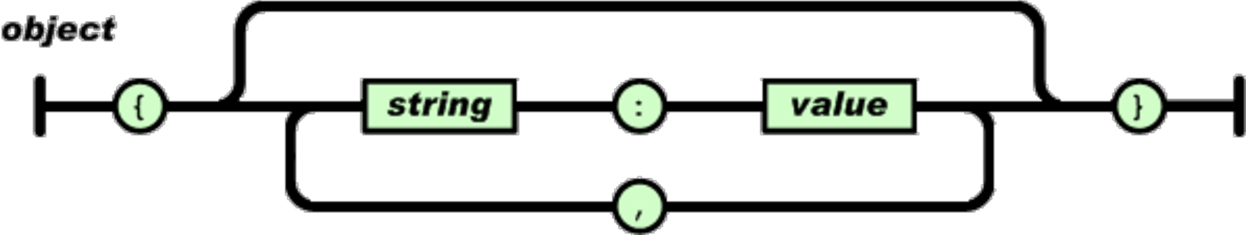
\includegraphics[width=400px]{00_media/03_objetJson.pdf}
      \caption{Diagramme syntaxique pour objet JSON tiré du site \cite{online:jsonorg}}
      \label{gra:jsonsyntax}
\end{figure}

\subsubsection{Tableau JSON}
Un tableau est une collection de valeurs. Il commence par une accolade ouvrante (\texttt{\{}) et se termine par une accolade fermante (\texttt{\}}). La figure \ref{gra:jsonsyntaxarray} illustre un diagramme syntaxique rendant valide un tableau \gls{json}.

\begin{figure}[H]
      \centering
      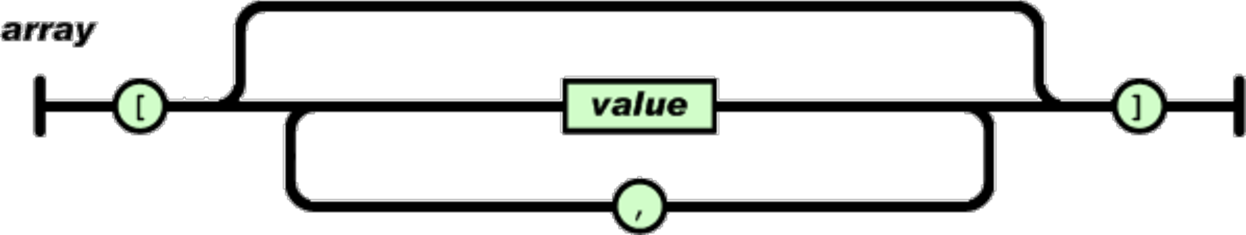
\includegraphics[width=400px]{00_media/03_arrayJson.pdf}
      \caption{Diagramme syntaxique pour array JSON tiré du site \cite{online:jsonorg}}
      \label{gra:jsonsyntaxarray}
\end{figure}
\subsubsection{Valeurs possibles}
Les valeurs peuvent être : 

\medskip

\begin{itemize}
  \item une chaîne de caractères délimité par des guillemets
  \item un nombre
  \item true
  \item false
  \item null
  \item un autre objet \gls{json}
  \item un tableau \gls{json}
\end{itemize}

\subsubsection{Exemple}
Le code \ref{lst:codeJsonExample} montre un exemple de structure \gls{json} et le code \ref{lst:codeXMLExample} son équivalent au format \emph{\gls{xml}}.
\begin{lstlisting}[language={XML}, caption={Exemple code JSON}, label={lst:codeJsonExample}]
{   "personne" :
          {     
                "prenom": "John",
                "nom" : "Doe",
                "age" : "42"
          }
}
\end{lstlisting}

\begin{lstlisting}[language={XML}, caption={Comparaison XML-JSON}, label={lst:codeXMLExample}]
<personne>
  <prenom>John</prenom>
  <nom>Doe</nom>
  <age>42</age>
</personne>
\end{lstlisting}

\subsubsection{Objectify}
Il existe un utilitaire intéressant qui permet de convertir du code \gls{json} en classe codé en \emph{\gls{obj-c}}. Cette utilitaire se nomme \emph{Objectify} et est disponible sur le site \cite{online:objectify}.

\medskip

Pour montrer de quoi est capable ce programme, j'ai repris le code \ref{lst:codeJsonExample} et le résultat de l'opération peut être visible sur le code \ref{lst:objectifya} pour le fichier \emph{header} et \ref{lst:objectifyb} pour le fichier d'implémentation.

\medskip

Comme le montre les résultats, ce programme peut nous faire gagner du temps pour concevoir les entités de notre application. Si cela est utilisé, il y aura cependant des modifications à faire au code car on peut voir que l'\emph{\gls{arc}} n'est pas utilisé puisqu'il y a des mots clefs comme \texttt{retain, release, autorelease} qui prouvent que la mémoire est gérée manuellement et non en profitant de \emph{\gls{arc}}.

\begin{lstlisting}[language={JAVA}, caption={Objectify - Resultat du fichier.h}, label={lst:objectifya}]
#import <Foundation/Foundation.h>
@interface MyClass : NSObject {
    NSString *age;
    NSString *nom;
    NSString *prenom;
}
@property (nonatomic, copy) NSString *age;
@property (nonatomic, copy) NSString *nom;
@property (nonatomic, copy) NSString *prenom;
+ (MyClass *)instanceFromDictionary:(NSDictionary *)aDictionary;
- (void)setAttributesFromDictionary:(NSDictionary *)aDictionary;
@end
\end{lstlisting}

\begin{lstlisting}[language={JAVA}, caption={Objectify - Resultat du fichier.m}, label={lst:objectifyb}]
#import "MyClass.h"
@implementation MyClass
@synthesize age = age;
@synthesize nom = nom;
@synthesize prenom = prenom;
- (void)dealloc {
    [age release], age = nil;
    [nom release], nom = nil;
    [prenom release], prenom = nil;
    [super dealloc];
}
+ (MyClass *)instanceFromDictionary:(NSDictionary *)aDictionary {
    MyClass *instance = [[[MyClass alloc] init] autorelease];
    [instance setAttributesFromDictionary:aDictionary];
    return instance;
}
- (void)setAttributesFromDictionary:(NSDictionary *)aDictionary {
    if (![aDictionary isKindOfClass:[NSDictionary class]]) {
        return;
    }
    self.age = [aDictionary objectForKey:@"age"];
    self.nom = [aDictionary objectForKey:@"nom"];
    self.prenom = [aDictionary objectForKey:@"prenom"];
}
@end
\end{lstlisting}
\subsubsection{SBJson}
\emph{SBJson}, appelé avant \emph{json-framework}, est un parser \emph{\gls{json}} pour le langage \emph{\gls{obj-c}}. Une documentation est disponible sur le site \cite{online:sbjson}.

\medskip

Un test technologique a été fait afin de voir comment fonctionnait ce framework. Pour commencer, il faut télécharger le projet disponible sur le site \cite{online:sbjson} et suivre le tutorial disponible sur le site \cite{online:sbjsonproject}. On peut ainsi insérer dans la classe avec laquelle on travaille l'import du fichier nécessaire pour employer le framework comme le montre le code \ref{lst:sbjsonimport}.

\begin{lstlisting}[language={JAVA}, caption={Import de l'interface SBJson}, label={lst:sbjsonimport}]
#import "SBJson/SBJsonParser.h"
\end{lstlisting}

Afin de tester, le code \ref{lst:codeJsonExample} a été repris dans le but d'afficher les valeurs pour chaque clef. Le code \ref{lst:testtechnosbjson} montre l'implémentation qui a été faite et le résultat peut être visible en \ref{lst:testtechnosbjsonb}.

\begin{lstlisting}[language={JAVA}, caption={Test technologique pour SBJson}, label={lst:testtechnosbjson}]
// On initialise le parser
SBJsonParser * myParser = [[SBJsonParser alloc]init];
NSString * myJSonString = @"{\"personne\" : {\"prenom\": \"John\",\"nom\": \"Doe\",\"age\": \"42\"}}";
// On utilise le parser pour creer un objet avec le string ci-dessus
NSDictionary *jsonObject = [myParser objectWithString:myJSonString error:NULL];
// On construit un dictionnaire pour la clef personne
NSDictionary* person = [jsonObject objectForKey:@"personne"];
// On affiche les elements en les appelant avec leur clef
NSLog(@"prenom:%@", [person objectForKey:@"prenom"]);
NSLog(@"nom:%@", [person objectForKey:@"nom"]);
NSLog(@"age:%@", [person objectForKey:@"age"]);
\end{lstlisting}

\begin{lstlisting}[language={JAVA}, caption={Test technologique pour SBJson - Résultat}, label={lst:testtechnosbjsonb}]
prenom:john
nom:doe
age:42
\end{lstlisting}

% section analyse (end)


%	%!TEX root = ../rapport.tex

\section{Conception}
\label{section:conception_client}
La section ci-dessous a comme objectif de mettre en avant les choix de conception pour l'application. Premièrement, des maquettes seront présentées. Ensuite, l'architecture sera expliqué au travers du \emph{Storyboard} et des différentes contrôlleurs qui composent l'application. Finalement, les entités de l'application ont été schématisées et détaillées.

\subsection{Maquettes} % (fold)
\label{sub:maquettes}

Ci-dessous les maquettes créées permettent de se donner une meilleure idée sur le visuel de l'application finale. Sauf contraintes techniques, l'application ressemblera, à quelques exceptions près, le plus possible à ces mauqettes.

\subsubsection{Authentification}
La figure \ref{gra:maqLogin} montre comment sera présentera l'écran qui permettra de s'authentifier pour entrer dans l'application. L'utilisateur entre son login et son mot de passe et clique sur le bouton login. Dans le cas où les informations sont fausses ou si quelque choses s'est mal passé, un message lui sera proposé.
\begin{figure}[H]
      \centering
      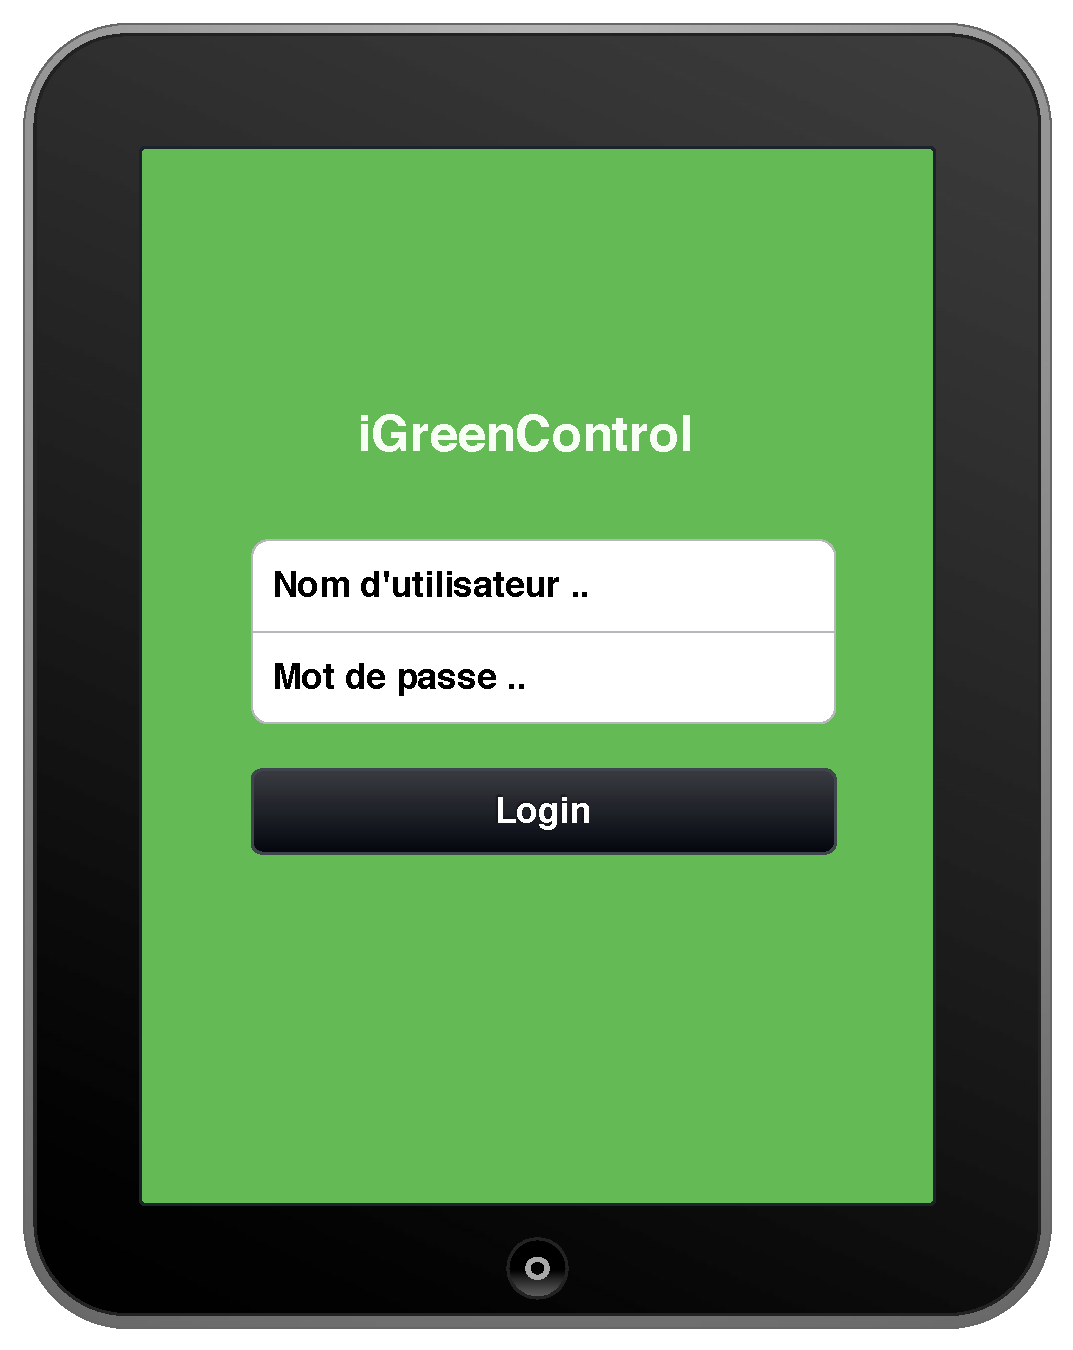
\includegraphics[width=8cm]{00_media/04_Maquette_00.pdf}
      \caption{Maquette - Login}
      \label{gra:maqLogin}
\end{figure}
\subsubsection{Menu général}
La figure \ref{gra:maqmenu} représente le menu de l'application. Celui-ci est composé de 6 boutons. Ci-dessous une description de ce qui est possible de faire avec chaque bouton.

\medskip

\begin{itemize}
  \item Le bouton \textbf{Maison} permet de lister les maisons dans le but d'en ouvrir une spécifique ou d'en créer une nouvelle
  \item Le bouton \textbf{Sauver} permet de sauver la maison en cours d'édition
  \item Le bouton \textbf{Importer plan} permet de choisir une image dans la librairie des photos de l'\emph{\gls{ipad}}.
  \item Le bouton \textbf{Insérer zone} permet d'insérer une nouvelle zone sur le plan ouvert
  \item Le bouton \textbf{Logout} permet de se déloguer et ainsi d'arriver à nouveau sur l'écran représenté par la figure \ref{gra:maqLogin} 
  \item Le bouton   \textbf{Infos} permet de voir des informations propres à l'application
\end{itemize}
\begin{figure}[H]
      \centering
      
\includegraphics[width=\textwidth]{00_media/04_Maquette_Menu.pdf}
      \caption{Maquette - Menu}
      \label{gra:maqmenu}
\end{figure}
\subsubsection{Menu pour les maisons}
La figure \ref{gra:maq01} sera l'écran visible quand l'utilisateur cliquera sur le bouton \textbf{Maison}. Il peut alors soit ouvrir une maison, soit créer une nouvelle maison.
\begin{figure}[H]
      \centering
      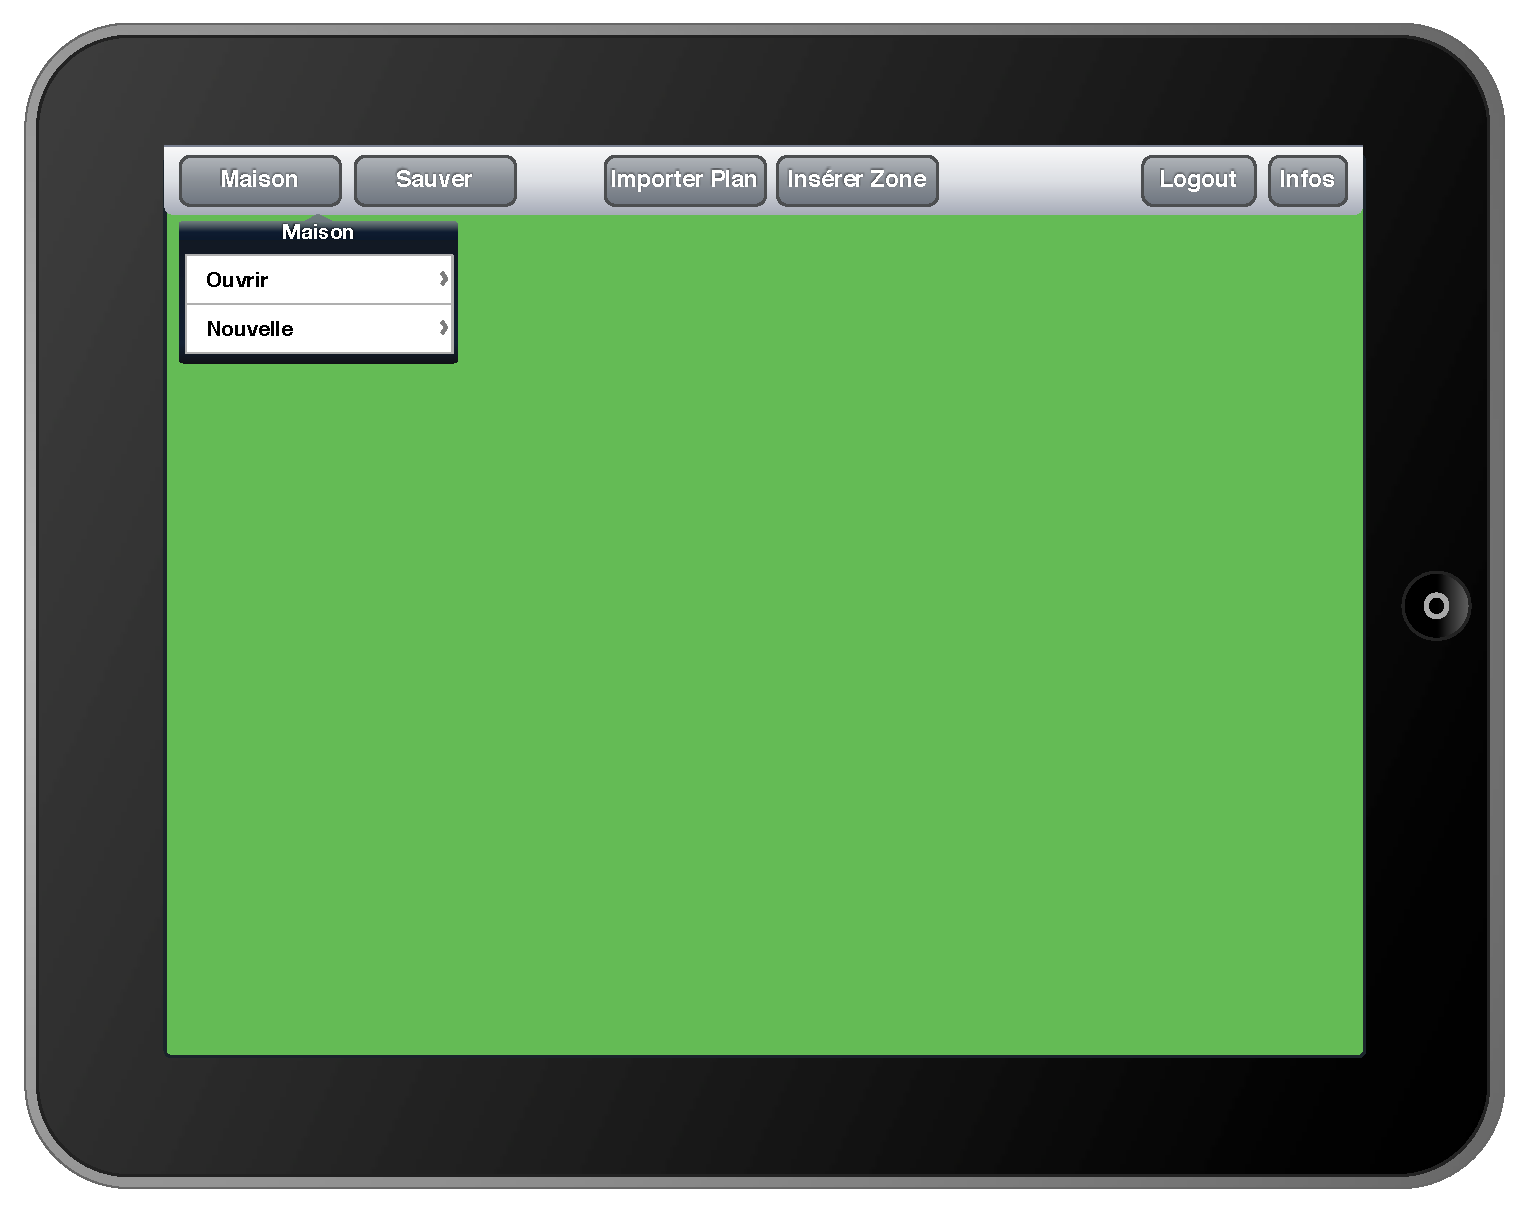
\includegraphics[width=9cm]{00_media/04_Maquette_01.pdf}
      \caption{Maquette - Menu Maison}
      \label{gra:maq01}
\end{figure}
\subsubsection{Lister les maisons}
La figure \ref{gra:maq02} propose la liste des maisons qui sont concernées par l'utilisateur loggué. S'il clique sur une maison, celle-ci s'ouvre dans l'application.

\medskip

Il peut également afficher le bouton pour supprimer une maison en passant son doigt de gauche à droite sur la maison.

\medskip

Un champ de recherche sera également présent dans le cas où l'utilisateur a beaucoup de maison et qu'il souhaite en rechercher une particulière.

\begin{figure}[H]
      \centering
      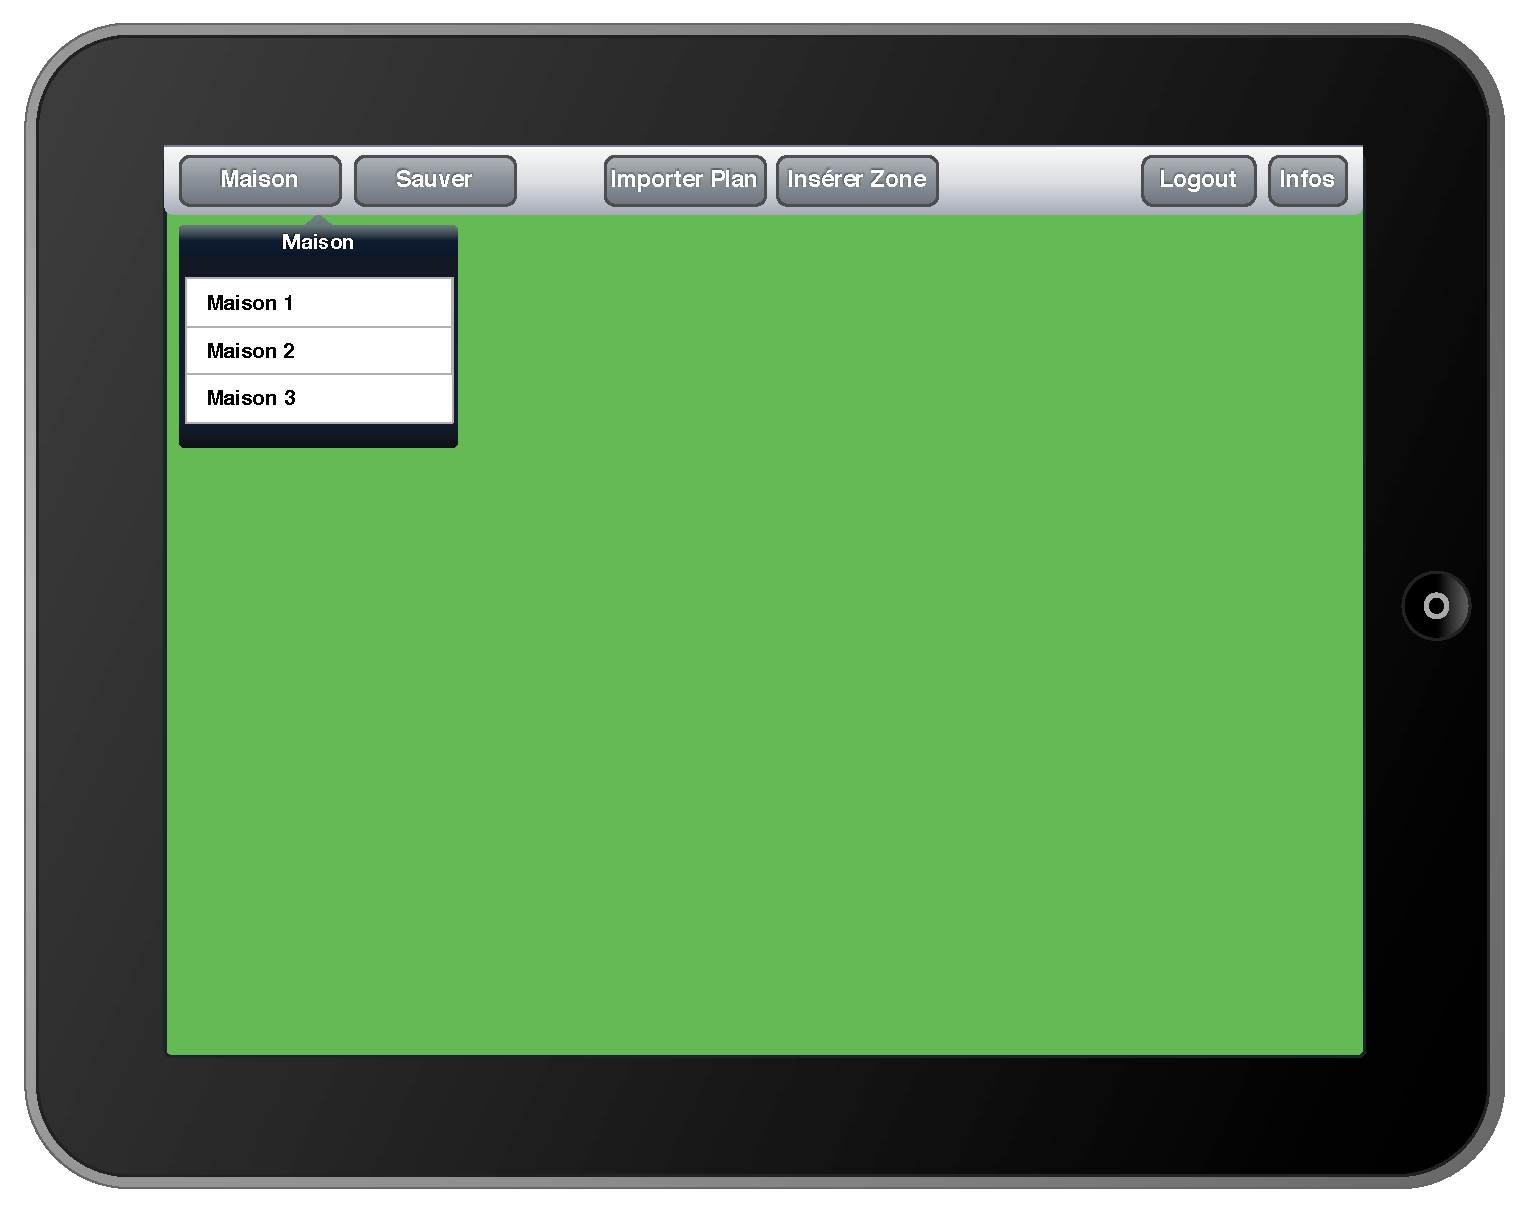
\includegraphics[width=9cm]{00_media/04_Maquette_02.pdf}
      \caption{Maquette - Liste Maison}
      \label{gra:maq02}
\end{figure}
\subsubsection{Créer une nouvelle maison}
La figure \ref{gra:maq03} apparaît si l'utilisateur clique sur nouvelle maison. Il doit alors entrer les informations qui sont utiles à la création de la maison puis cliquer sur le bouton pour sauvegarder la maison.
\begin{figure}[H]
      \centering
      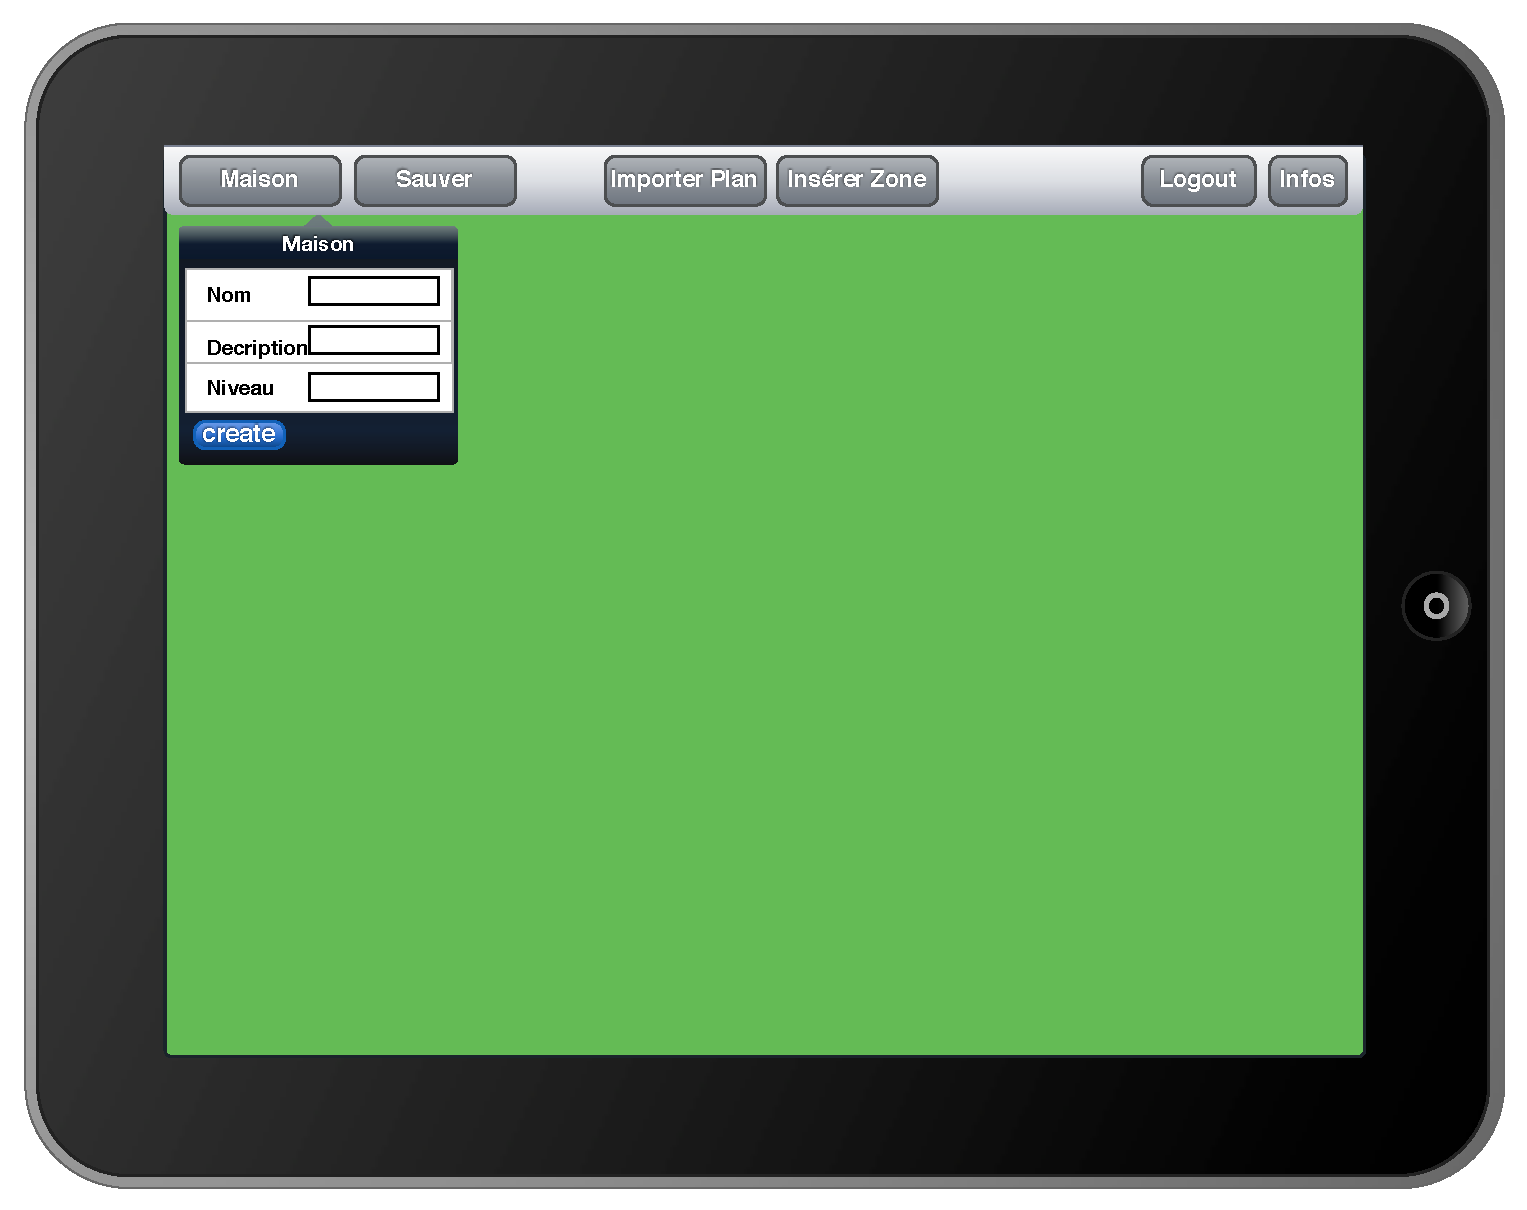
\includegraphics[width=9cm]{00_media/04_Maquette_03.pdf}
      \caption{Maquette - Nouvelle Maison}
      \label{gra:maq03}
\end{figure}
\subsubsection{Enregistrer une maison}
La figure \ref{gra:maq04} apparaît si l'utilisateur désire sauver la maison en cours. Il doit alors entrer les informations qu'il désire modifié puis cliquer sur le bouton pour sauvegarder la maison. Toutes les modifications effectuées seront alors sauvées.
\begin{figure}[H]
      \centering
      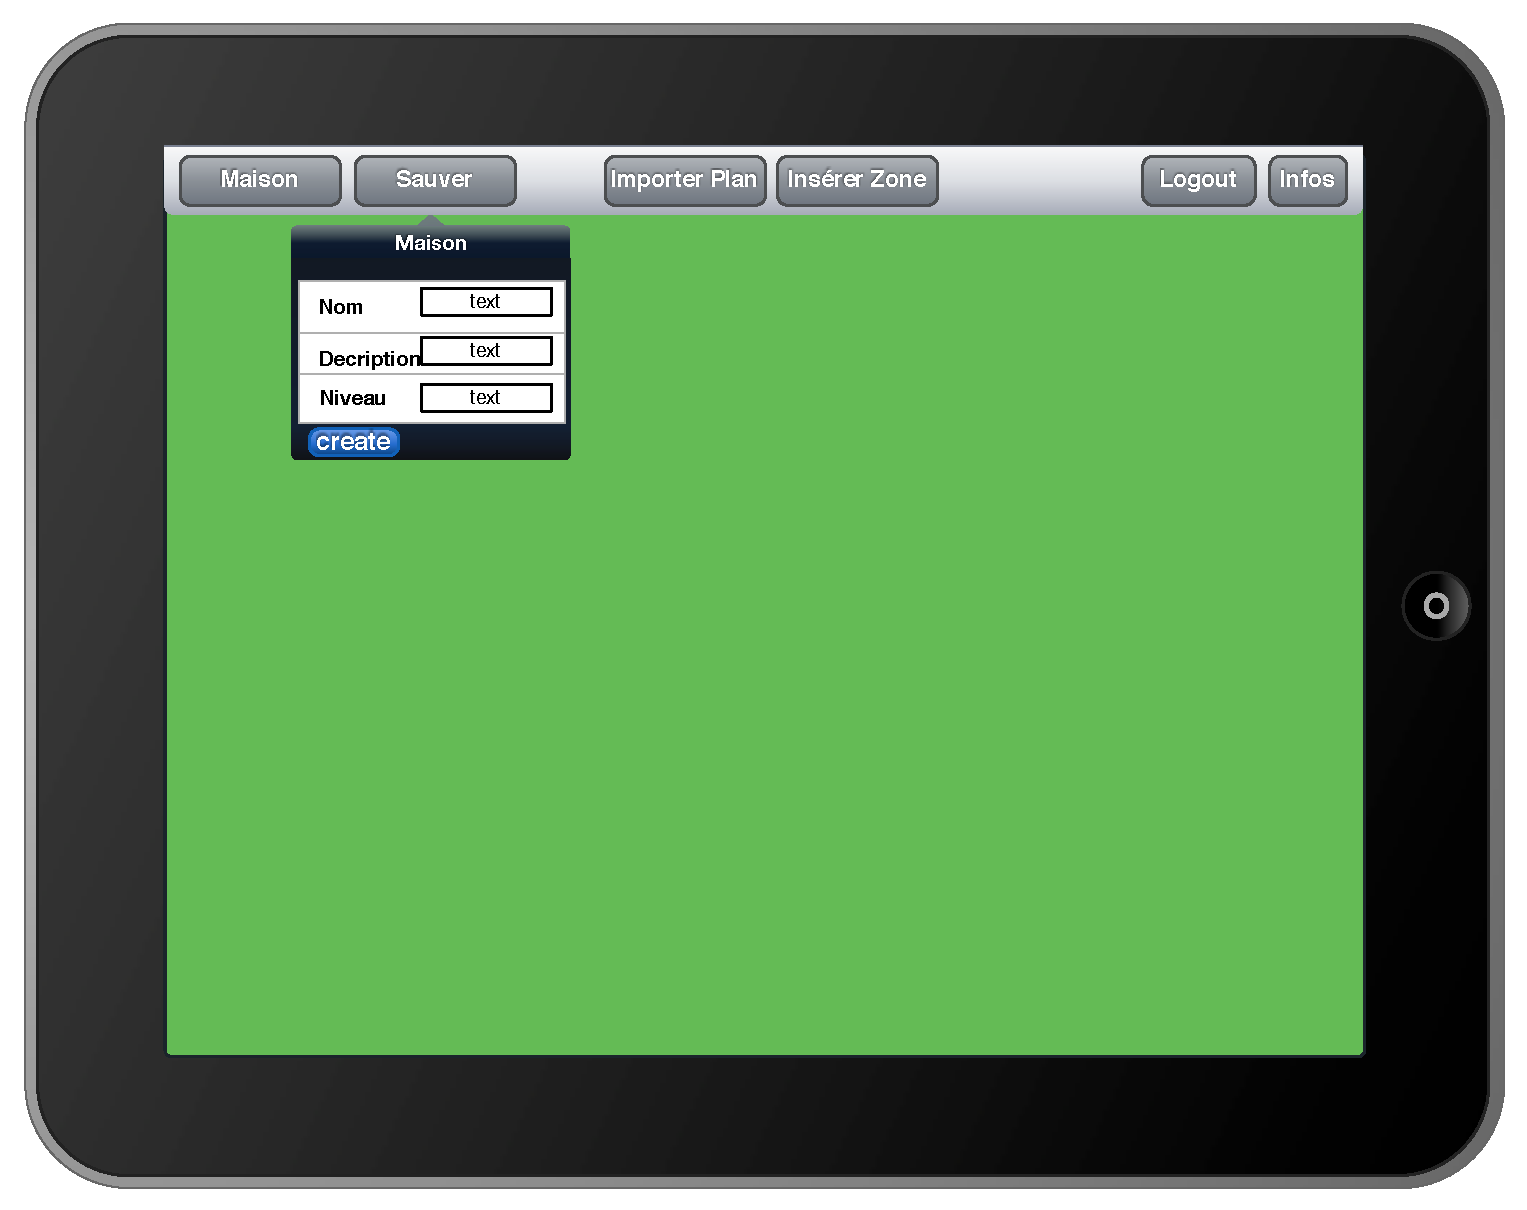
\includegraphics[width=9cm]{00_media/04_Maquette_04.pdf}
      \caption{Maquette - Sauver Maison}
      \label{gra:maq04}
\end{figure}
\subsubsection{Import d'une image}
La figure \ref{gra:maq05} intervient lorsque l'utilisateur veut importer un plan. Un explorateur d'images apparaît et il peut rechercher une photo qui est présente dans sa librairie de photos.
\begin{figure}[H]
      \centering
      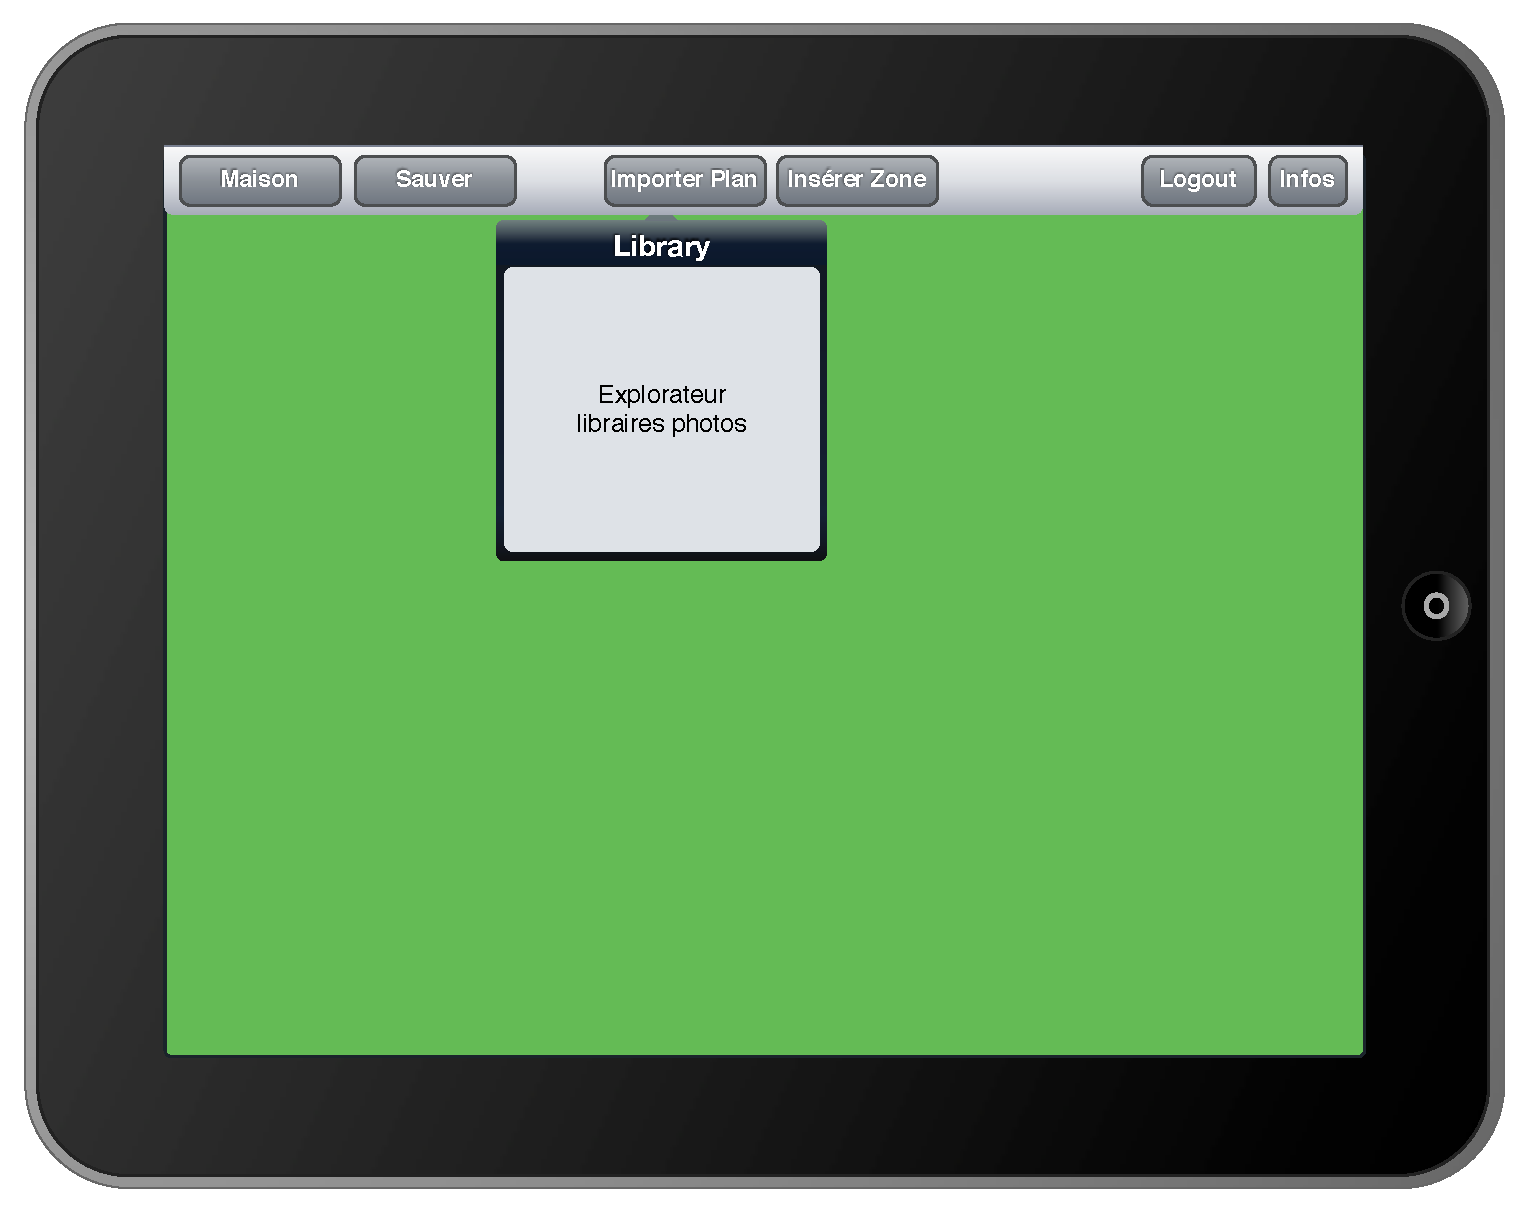
\includegraphics[width=9cm]{00_media/04_Maquette_05.pdf}
      \caption{Maquette - Import image}
      \label{gra:maq05}
\end{figure}
\subsubsection{Affichage du plan}
Quand une image a été selectionnée, celle-ci vient se position sur l'écran comme le montre la figure \ref{gra:maq06}. L'utilisateur pourra en modifier la position et la taille grâce à tes reconnaissances de gestes.
\begin{figure}[H]
      \centering
      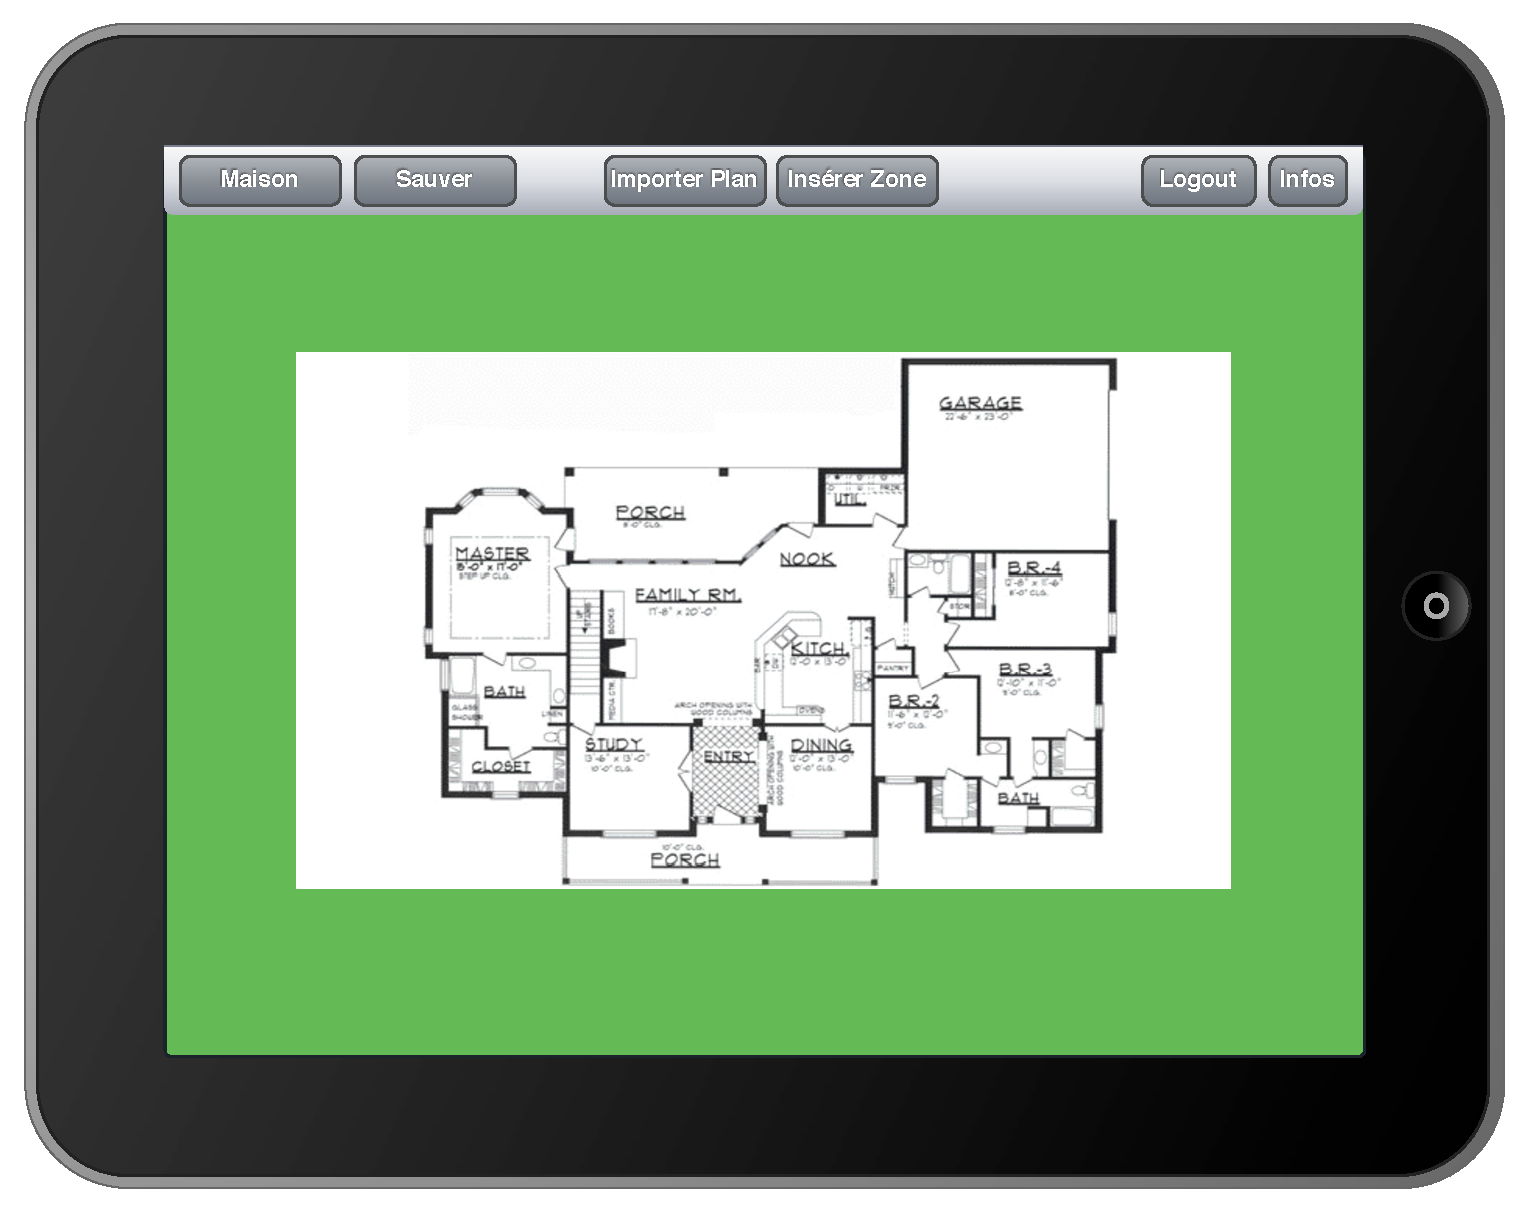
\includegraphics[width=9cm]{00_media/04_Maquette_06.pdf}
      \caption{Maquette - Plan}
      \label{gra:maq06}
\end{figure}
\subsubsection{Insertion d'une nouvelle zone}
Lorsque l'utilisateur veut insérer une nouvelle zone, il doit entrer des paramètres correspondant à la zone puis cliquer sur le bouton comme le montre la figure \ref{gra:maq07}.
\begin{figure}[H]
      \centering
      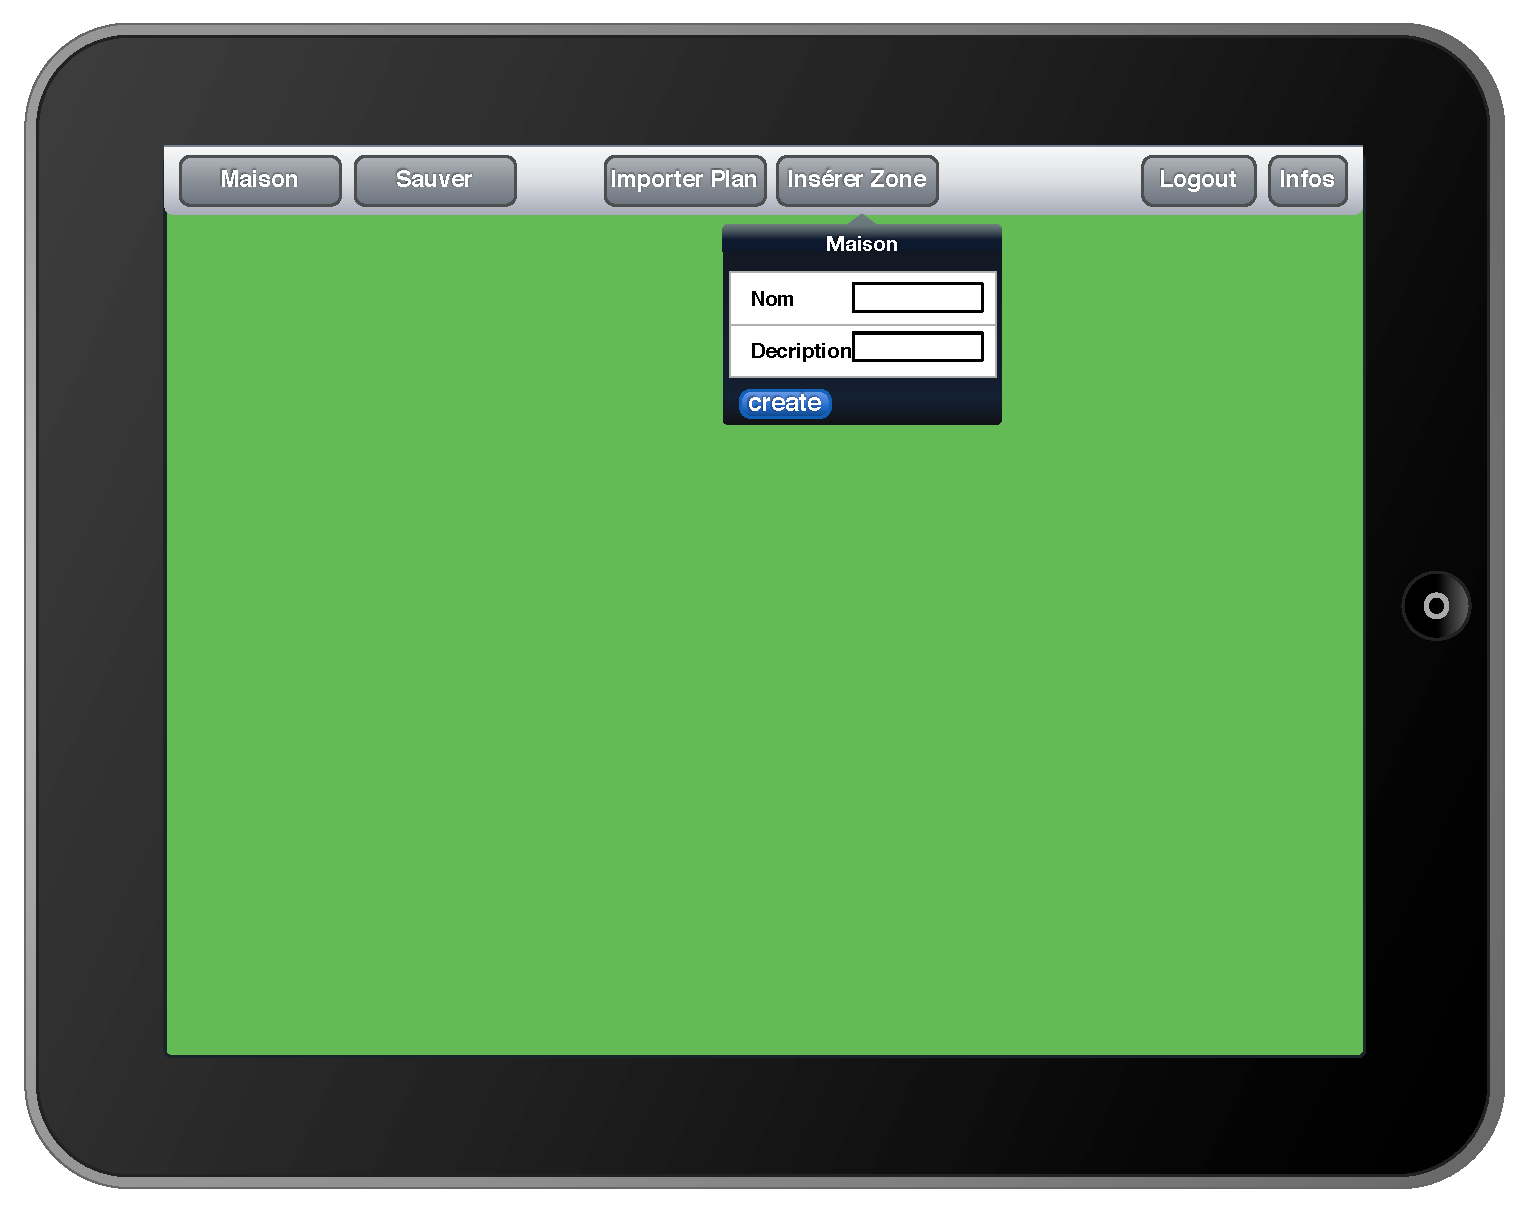
\includegraphics[width=9cm]{00_media/04_Maquette_07.pdf}
      \caption{Maquette - Nouvelle zone}
      \label{gra:maq07}
\end{figure}
\subsubsection{Représentation des zones}
Lorsque la zone a été insérée, elle peut être visible par un rectangle sur le plan comme le montre la figure \ref{gra:maq08}. La zone peut être redimensionnée ou déplacée. On peut même la faire pivoter grâce à des reconnaissances de gestes.

\begin{figure}[H]
      \centering
      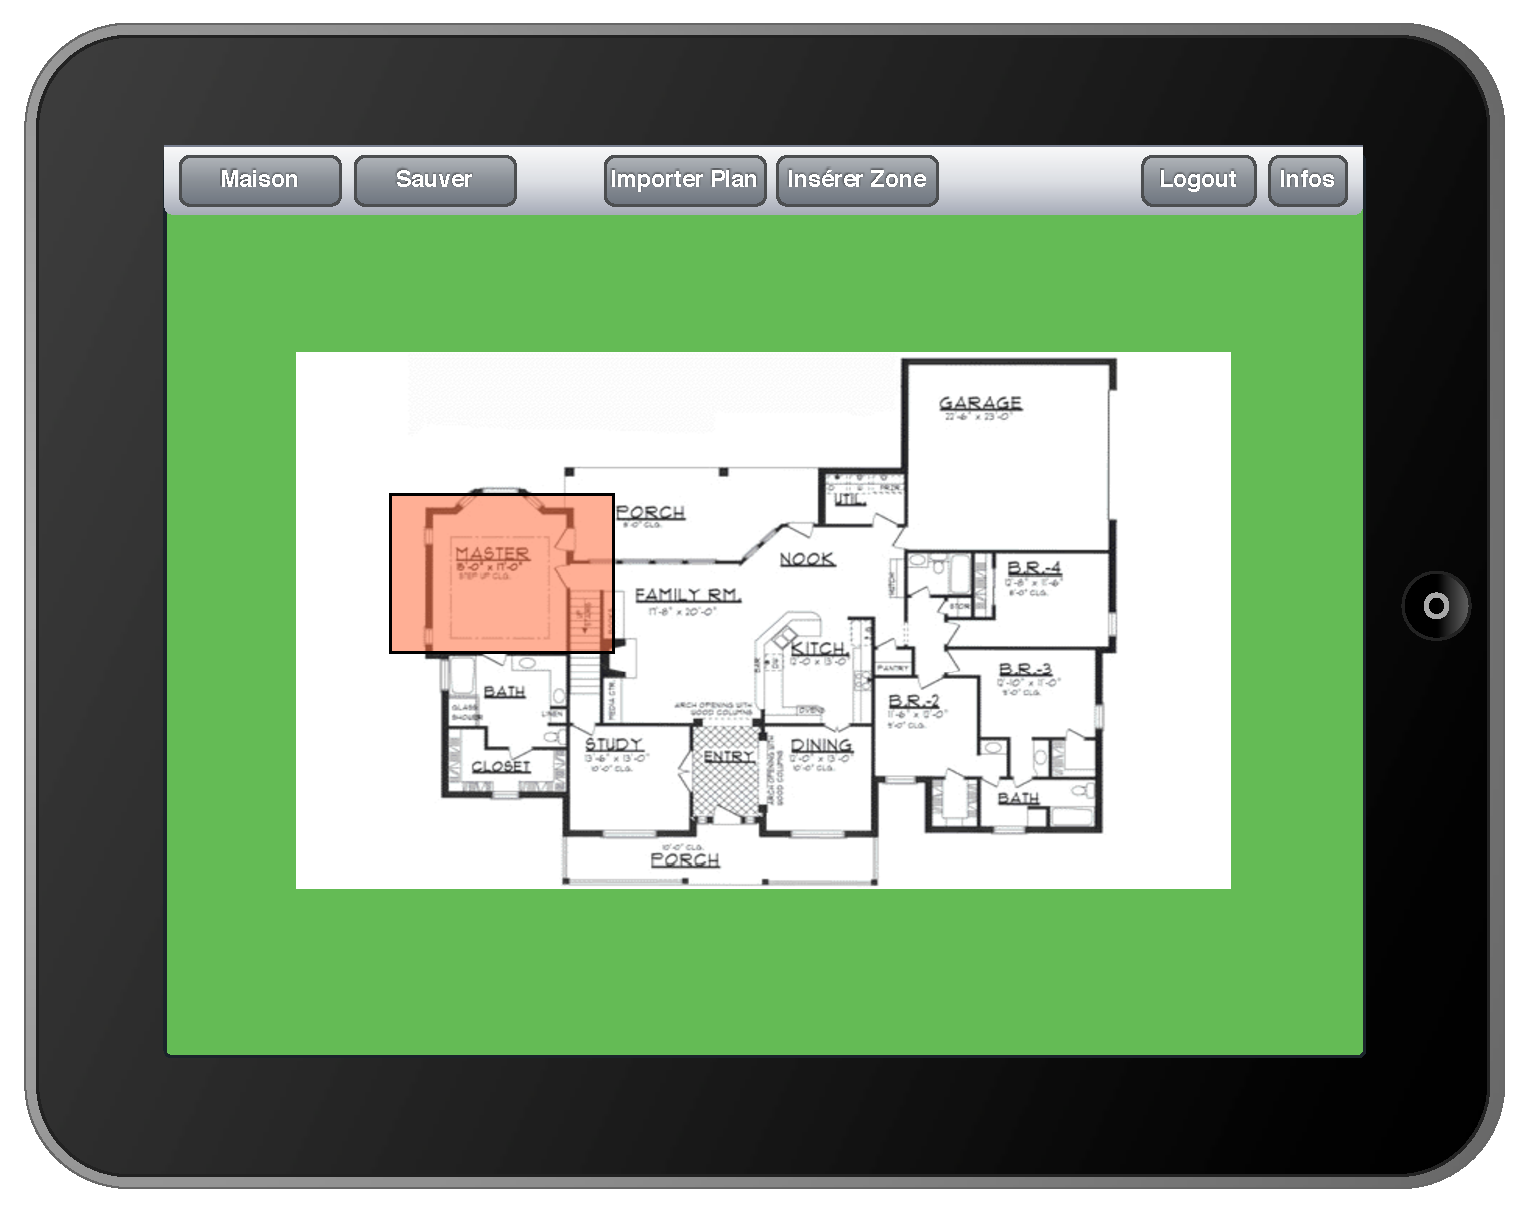
\includegraphics[width=9cm]{00_media/04_Maquette_08.pdf}
      \caption{Maquette - Zone}
      \label{gra:maq08}
\end{figure}
\subsubsection{Options sur les zones}
Lorsque l'utilisateur presse un certain moment sur une zone, un menu apparaît comme sur la figure \ref{gra:maq09}. Il peut alors modifier les paramètres de la zone comme le nom, la description et d'autres informations. Il peut également supprimer la zone ou insérer un capteur dans la zone.
\begin{figure}[H]
      \centering
      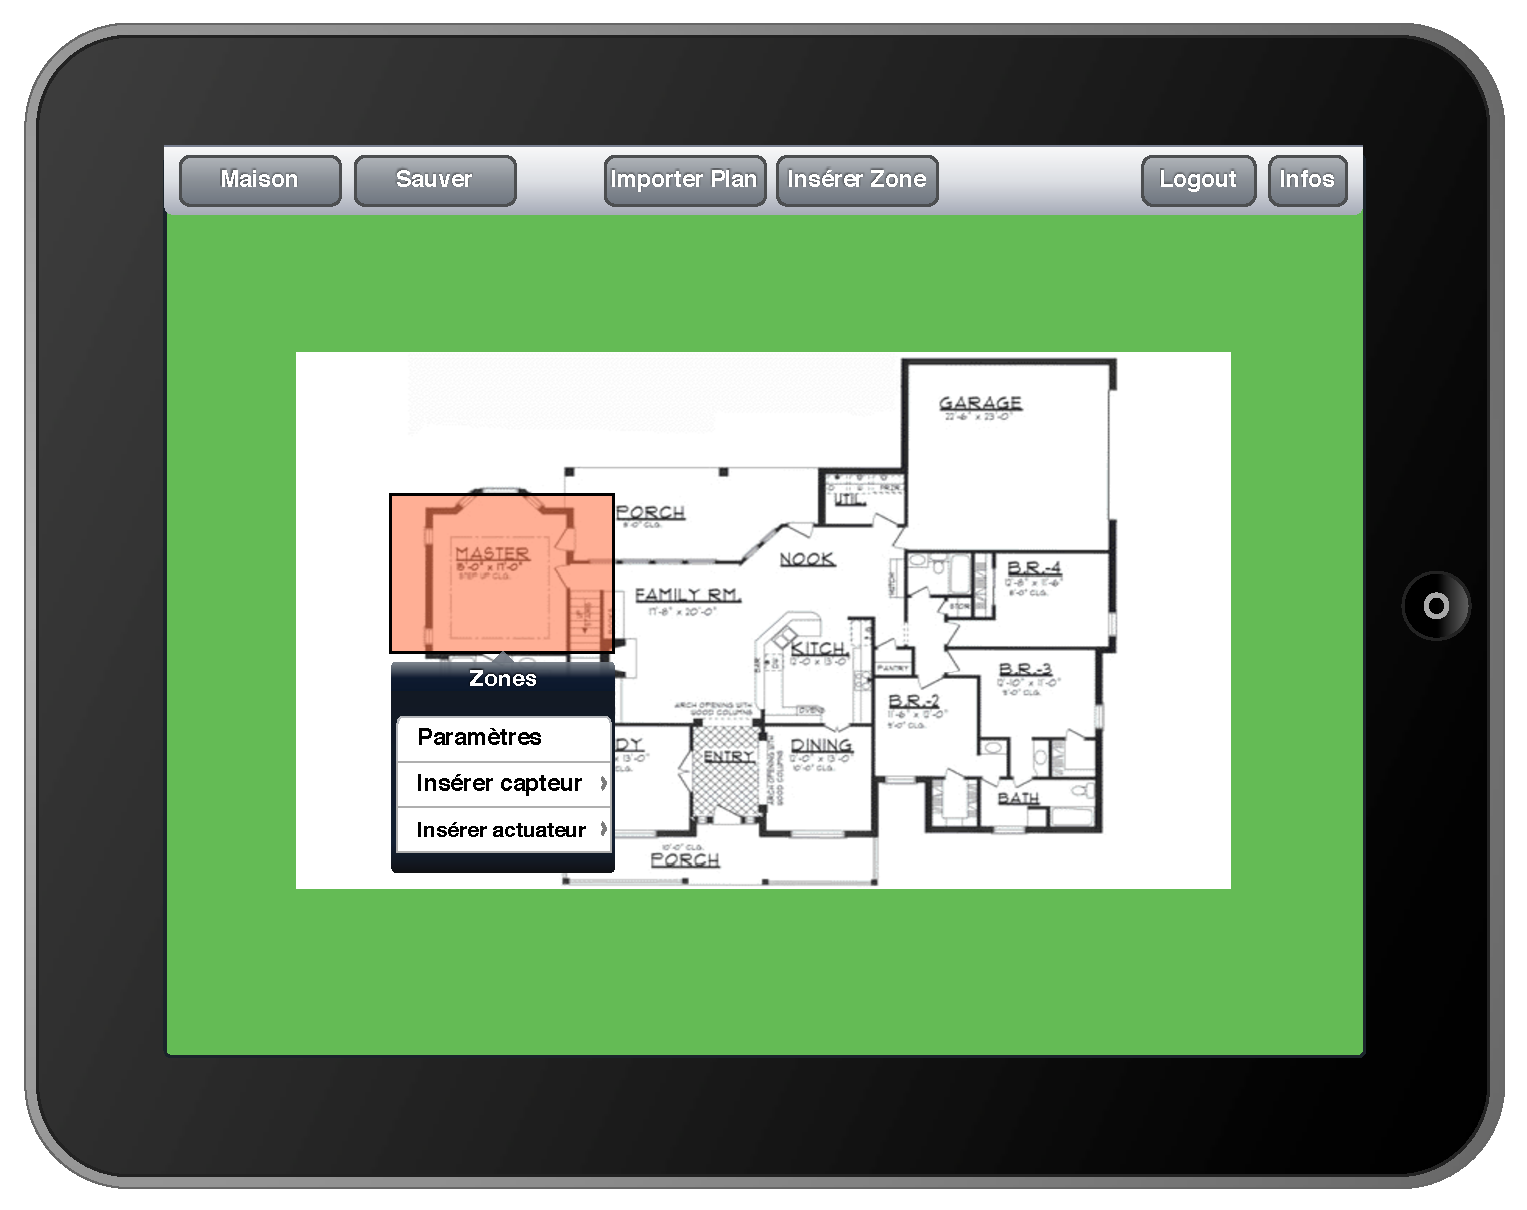
\includegraphics[width=9cm]{00_media/04_Maquette_09.pdf}
      \caption{Maquette - Options sur une zone}
      \label{gra:maq09}
\end{figure}
\subsubsection{Représentation des capteurs}
Lorsqu'un capteur est inséré, il est représenté directement dans la zone correspondante. Le rectangle bleu de la figure \ref{gra:maq10} représente un capteur.
\begin{figure}[H]
      \centering
      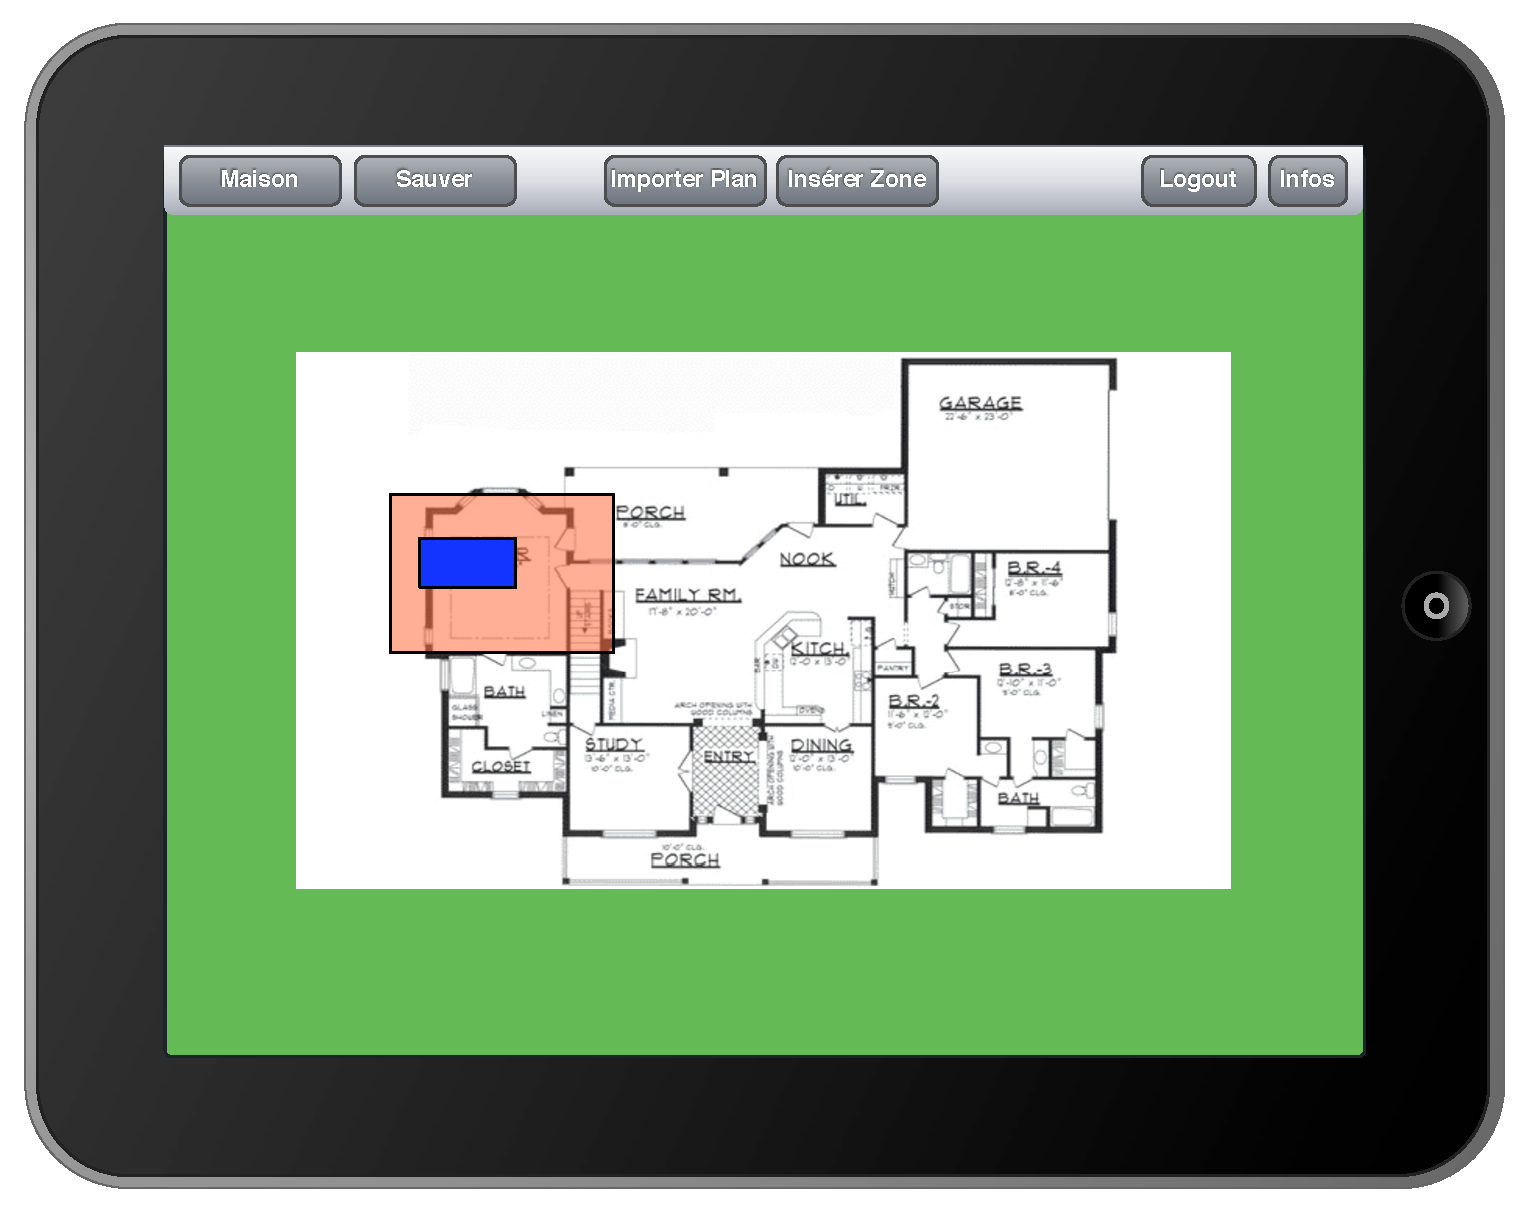
\includegraphics[width=9cm]{00_media/04_Maquette_10.pdf}
      \caption{Maquette - Capteur}
      \label{gra:maq10}
\end{figure}
\subsubsection{Options sur les capteurs}
Lorsque l'utilisateur presse un certain temps sur un capteur, un menu apparaît et permet d'effectuer des opération sur le capteur correspondant. Ceci est représenté par la figure \ref{gra:maq11}. Il peut le supprimer, en modifier les paramètres ou voir les données du capteur.
\begin{figure}[H]
      \centering
      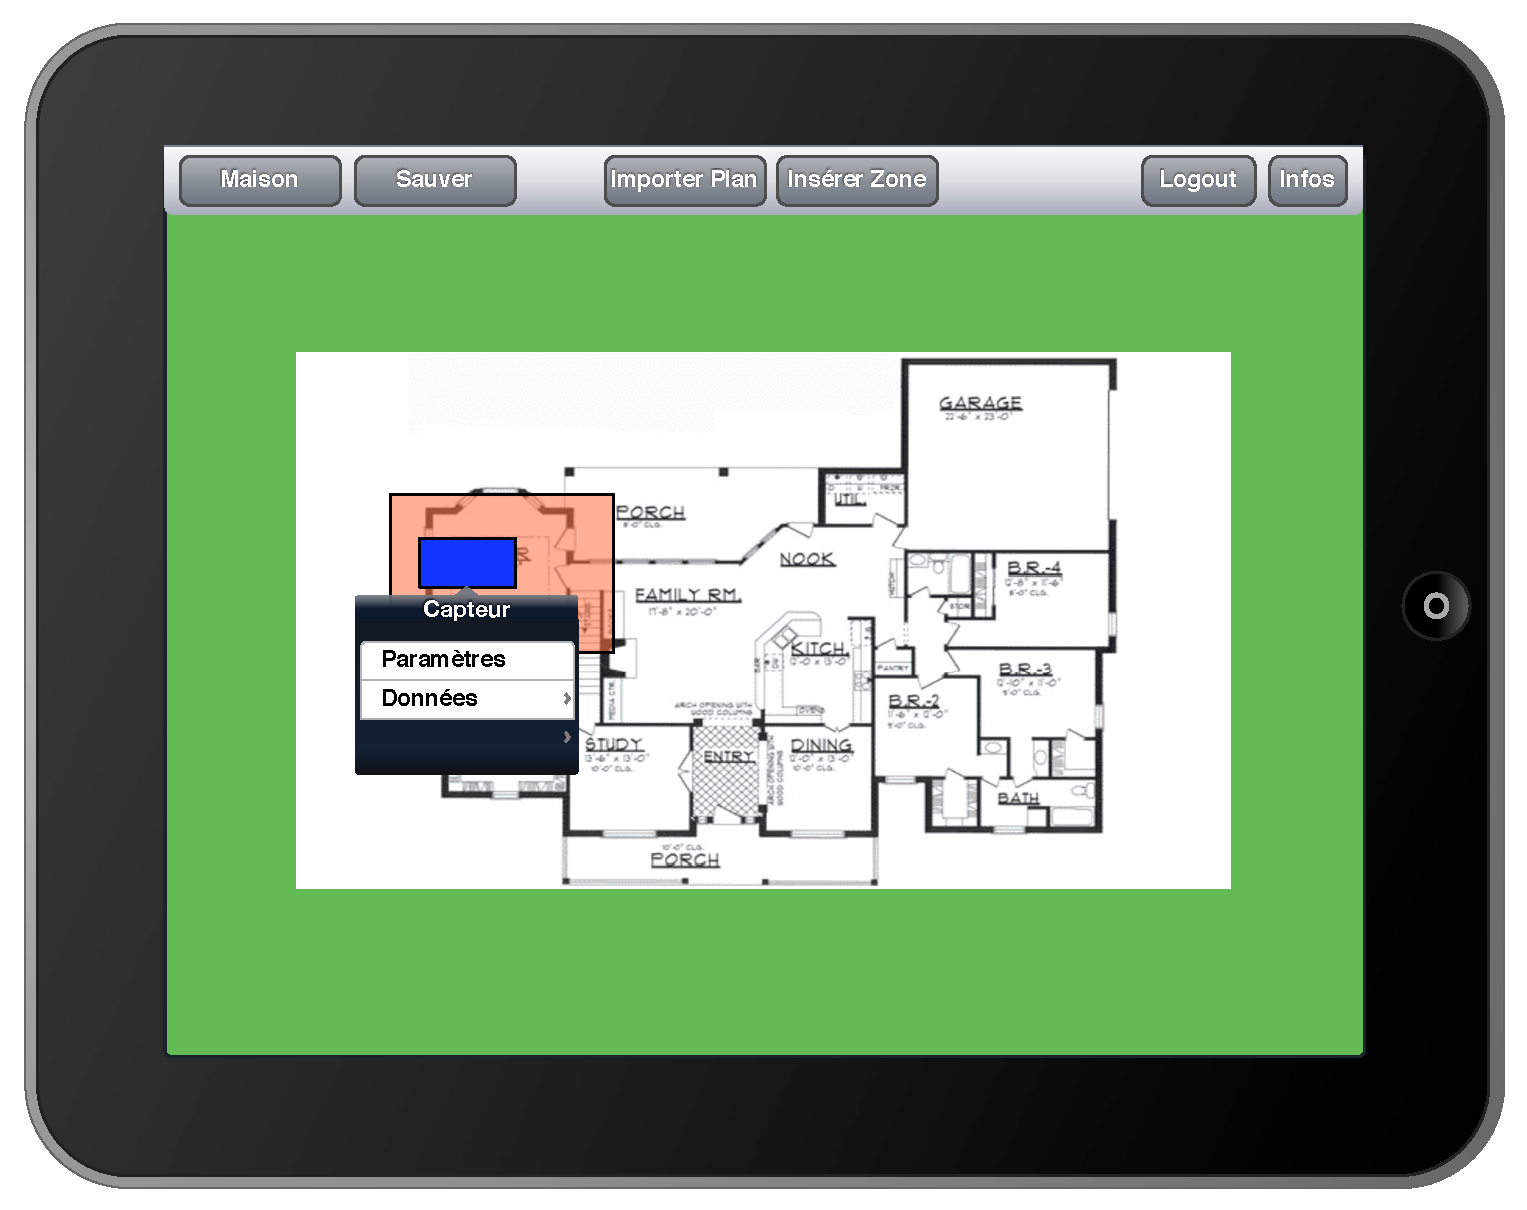
\includegraphics[width=9cm]{00_media/04_Maquette_11.pdf}
      \caption{Maquette - Options sur capteur}
      \label{gra:maq11}
\end{figure}
\subsubsection{Informations sur l'application}
La figure \ref{gra:maq12} montre le \emph{About} de l'application. L'utilisateur pourra lire des informations relatives à l'application.
\begin{figure}[H]
      \centering
      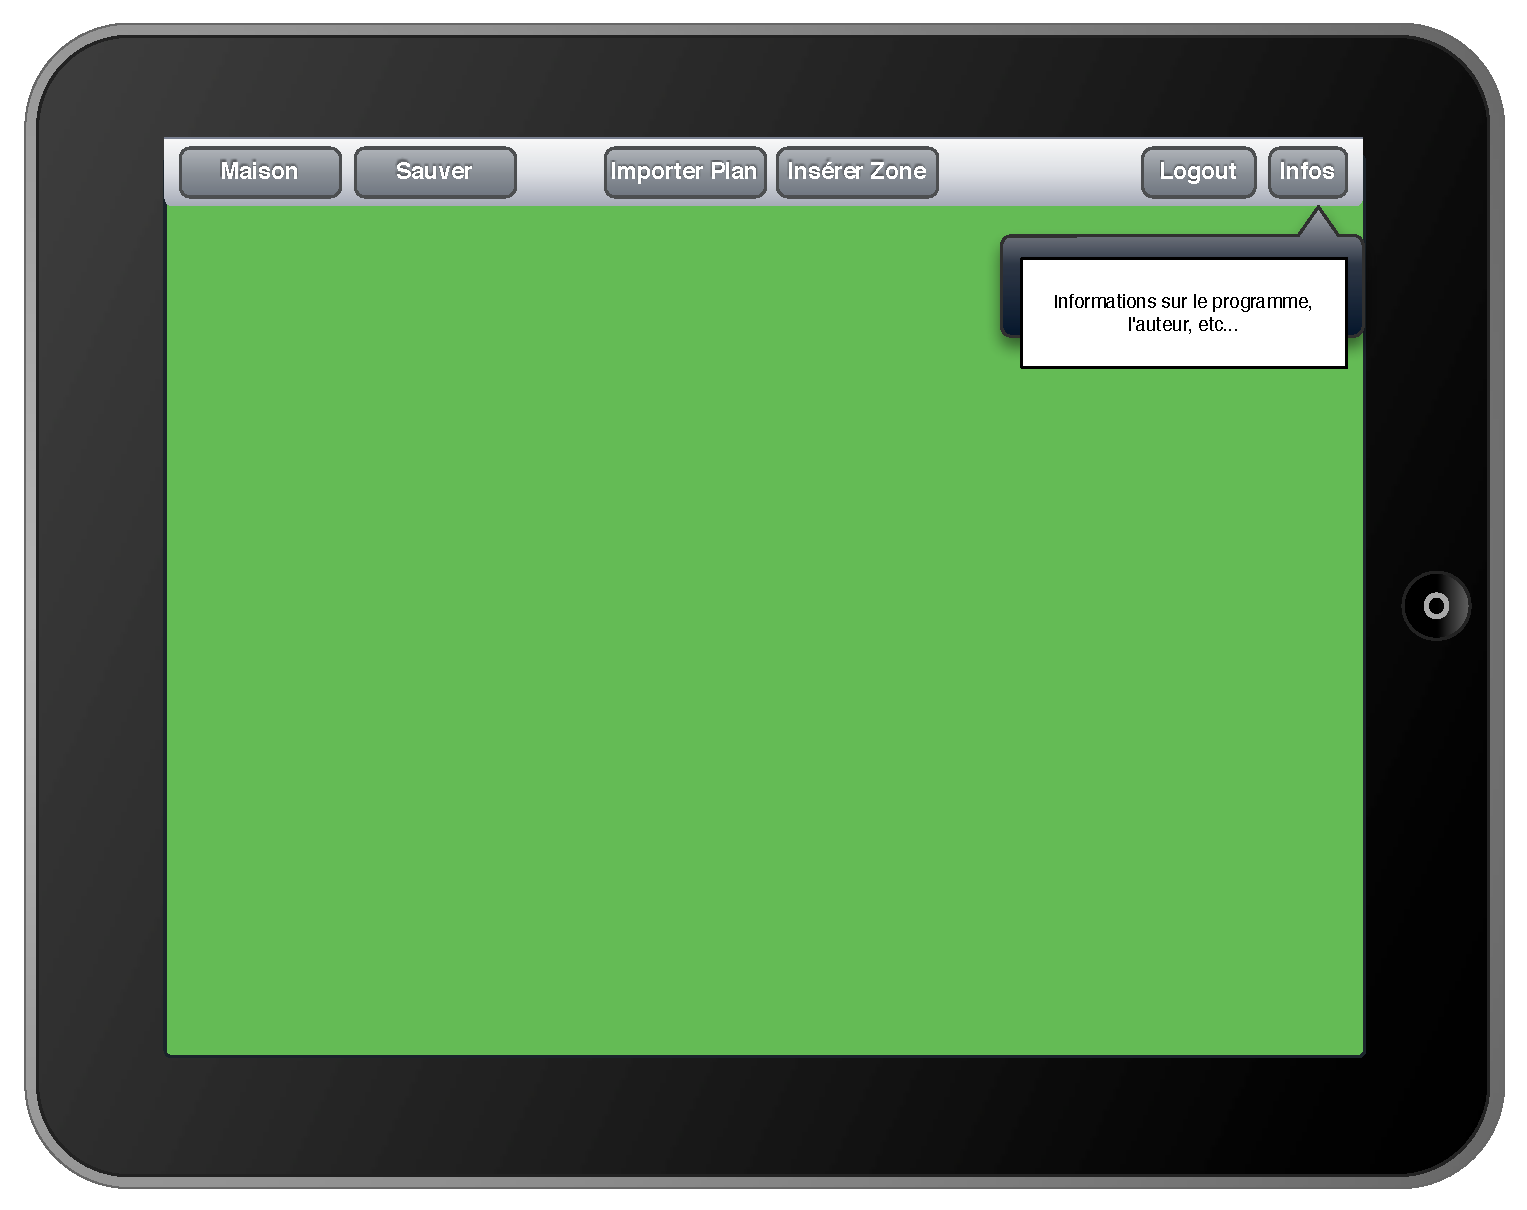
\includegraphics[width=9cm]{00_media/04_Maquette_12.pdf}
      \caption{Maquette - Infos}
      \label{gra:maq12}
\end{figure}

\subsubsection{Supprimer les maisons}

Afin de supprimer les maisons, il suffira de faire un défilement de gauche à droite sur la maison désirée se trouvant dans la liste. Un bouton "supprimer" apparaîtra alors.

\subsection{Mode paysage / portrait}
L'application sera conçue pour être utiliser en mode paysage. Le seul écran qui pourra être en mode paysage et portrait est lorsque l'utilisateur veut se logguer.

\subsection{Architectures de l'application} % (fold)
\label{sub:architectures_de_l_application}

L'application a été découpé en 3 parties bien distinctes.

\medskip

\begin{itemize}
  \item Un dossier \emph{Model} regroupe les entités de l'application (User, House, Zone, Sensor, SensorData)
  \item Un dossier \emph{Controller} regroupe tous les contrôleurs de l'application
  \item Un dossier \emph{Delegate} regroupe tous les delegate de l'application
\end{itemize}

% subsection architectures_des_c (end)

\subsection{Architecture des contrôleurs} % (fold)
\label{sub:architecture_de_l_application}
Les contrôleurs permettent en résumé d'afficher les vues de l'application

\medskip

La figure \ref{gra:iGreencontrolStoryboard} représente le \emph{Storyboard} de l'application. En guise d'explicatif de l'architecture de l'application, je vais détailler ici comment les différentes vues ont été conçues.

\medskip

Le première écran, le login, est un contrôleur de type \emph{UIViewController}.

\medskip

L'écran principal de l'application, celui ou sera affiché les plans, les zones, etc.. est un contrôleur de type \emph{UIViewController}.

\medskip

Le contrôleur qui englobe le menu qui permet de gérer la liste des maisons et d'en créer est un \emph{UINavigationController} qui permet notamment de faire des transitions entre différents contrôleurs. C'est d'ailleurs pour cela que j'ai utilisé ceci puisque le menu, le formulaire pour créer une nouvelle maison et la liste des maisons sont des \emph{UITableViewController}.

\medskip

Pour ce qui est de l'insertion d'une zone et de la sauvegarde d'une maison, le contrôleur est également un \emph{UITableViewController}.

\medskip

Pour afficher les informations lorsque l'utilisateur clique sur le bouton \emph{Infos}, il s'agit d'un \emph{UIViewController}.

\medskip

Il y a des éléments qui ne sont pas représentés sur le \emph{Storyboard} car ils sont créés dynamiquement comme par exemple les menus lorsqu'on appuie longtemps sur une zone ou sur un capteur. Ce sont des \emph{UINavigationController} qui englobent à chaque fois des \emph{UITableViewController} pour lister des ressources et afficher les formulaires.

\medskip

Pour afficher tout les éléments cités ci-dessus, des \emph{UIPopoverController} ont été employé. Ces derniers permettent d'afficher une sorte de popup et de les initialiser avec un contrôleur.

\begin{figure}[H]
      \centering
      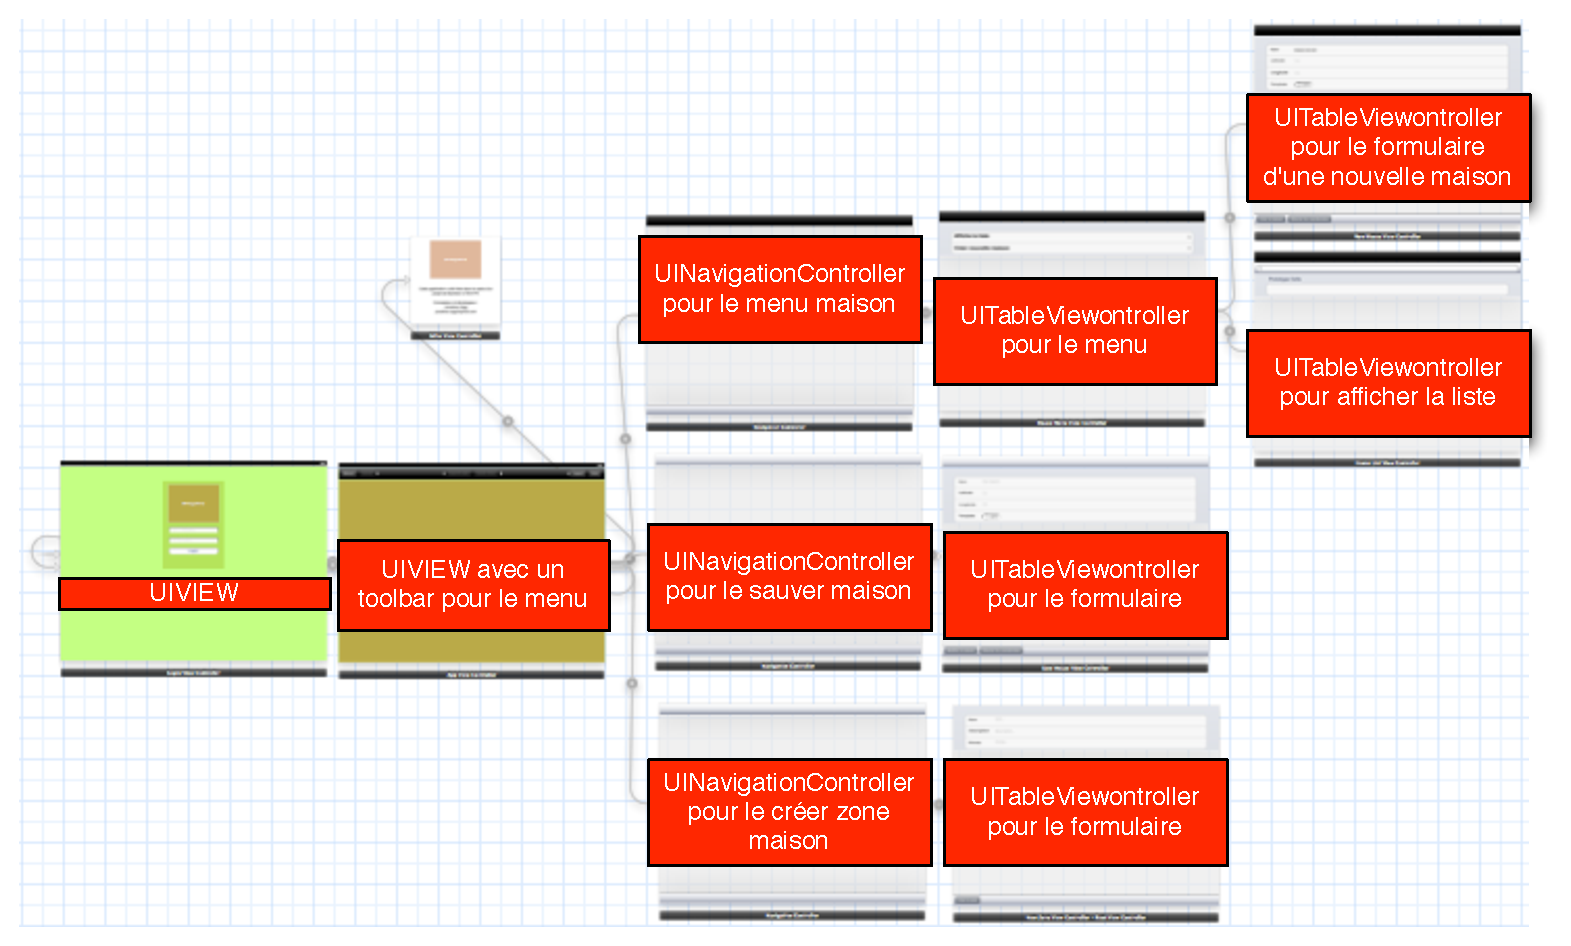
\includegraphics[angle=0,width=13 cm]{00_media/04_storyboard.pdf}
      \caption{Storyboard de l'application iGreenControl}
      \label{gra:iGreencontrolStoryboard}
\end{figure}
% subsection architecture_de_l_application (end)


\subsection{Vue logique des entités de l'application} % (fold)
\label{sub:vue_logique}

La figure \ref{gra:vueLogApp} illustre un diagramme de classes représentant les entités qui seront nécessaires à l'application. Le tableau \ref{tab:classDiagram} explique chaque entité.

\begin{figure}[H]
        \centering
        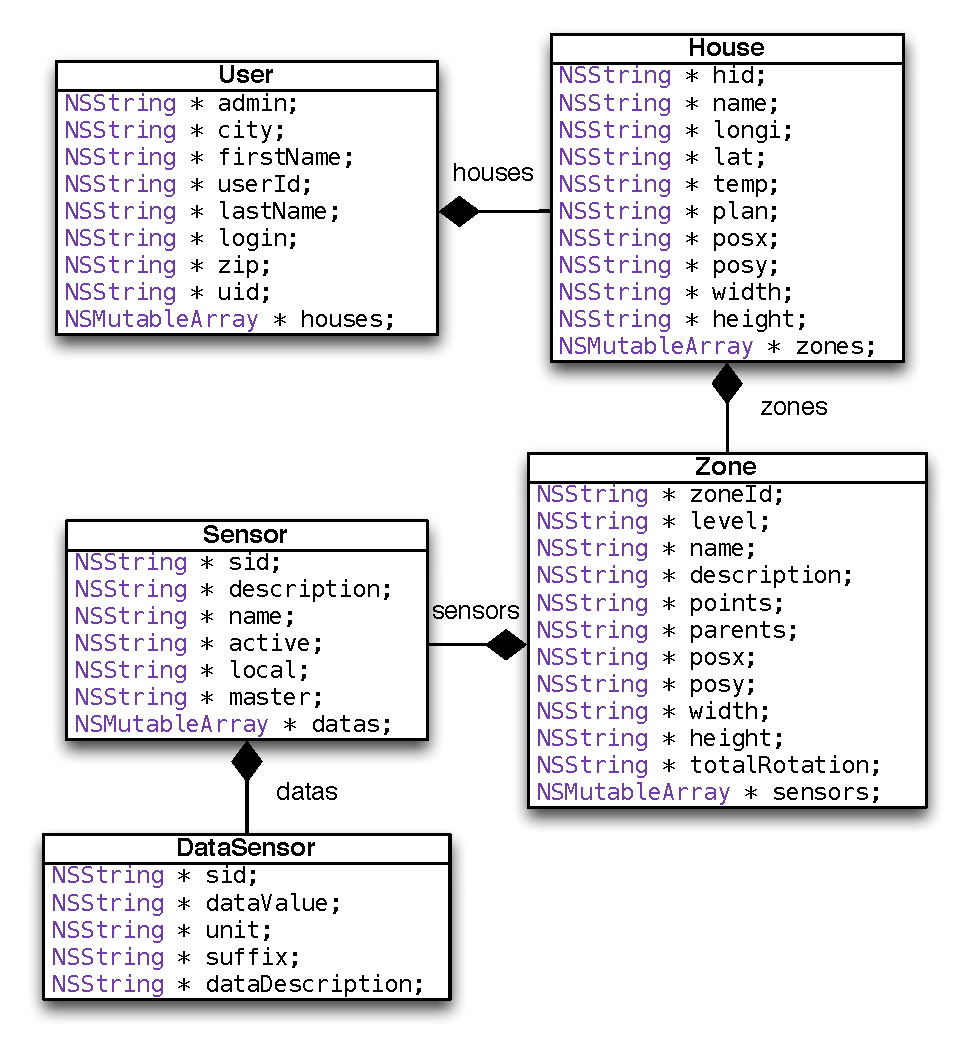
\includegraphics[width=11cm]{00_media/04_Client_Diagramme_classe_metier.pdf}
        \caption{Vue logique de l'application}
        \label{gra:vueLogApp}
\end{figure}

\begin{table}[H]
\begin{tabularx}{\textwidth}{|m{3cm}|X|l|}
  \hline
  \bf{Nom} & \bf{Description} \\
  \hline
  User & Cette entité permettra d'effectuer correctement l'authentification et de récupérer l'identification pour le bon déroulement du programme comme par exemple filtrer les maisons en affichant uniquement celles de l'utilisateur connecté. L'utilisateur disposera donc d'une liste de maison. \\
  \hline  
  House & Cette entité permettra d'effectuer des modifications sur les maisons comme par exemple en changer le nom ou l'image. Les valeurs comme width, height,  posx ou posy permettront de savoir ou positionner l'image du plan dans l'application L'entité contient également une liste de zones insérées par l'utilisateur.\\
  \hline  
  Zone & Cette entité permettra d'effectuer des modifications sur les zones insérées par l'utilisateur. Cela permettra également de savoir ou la zone est placée sur le plan et sa taille. Une zone pourra contenir des capteurs. \\
  \hline  
  Sensor & Cette entité représentera les capteurs. Elle permettra à l'utilisateur d'en changer les paramètres comme le nom, la description, etc... De plus un capteur contient des données qui sont représentées par l'entité DataSensor \\
  \hline  
  DataSensor & Cette entité représentera les données du capteurs. Plusieurs informations pourront être affichables comme par exemple la valeur, l'unité, la description, etc.. \\
  \hline
\end{tabularx}
\caption{Récapitualif du diagramme de classes}
\label{tab:classDiagram}
\end{table}

% subsection vue_logique (end)

%	%!TEX root = ../rapport.tex

\section{Réalisation}
Cette section a pour but de présenter certains détails jugés importants par rapport à l'implémentation.

\subsection{UIApplicationDelegate} % (fold)
\label{sub:uiapplicationdelegate}

J'ai créé une classe \emph{IGCAppDelegate} qui est en fait le delegate de l'application. En effet, cette classe suit le protocole \emph{UIApplicationDelegate} qui permet de gérer les différentes parties du cycle de vie d'une application.

\medskip 

Comme  il n'était pas utile de gérer le cycle de vie dans le projet. J'ai utilisé cette classe pour partager différentes informations à travers toutes les autres classes de mon application. 

\medskip

Cela est assez logique car c'est une classe qui est instanciée une seule et unique fois. On appelle cela un \emph{\gls{singleton}}. Afin de récupérer son instance, il est nécessaire d'employé le code \ref{lst:appDelegateSingleton} ci-dessous.

\begin{lstlisting}[language={JAVA}, caption={Récuperer l'instance de l'application delegate}, label={lst:appDelegateSingleton}]
IGCAppDelegate * appDelegate = (IGCAppDelegate*) [UIApplication sharedApplication].delegate;
\end{lstlisting}

J'utilise par exemple ce \emph{\gls{singleton}} pour : 

\medskip

\begin{itemize}
	\item Stocker le client \emph{Restkit} qui permet de faire des requêtes de type \emph{\gls{rest}}
	\item Stocker les informations de l'utilisateur qui est connecté
	\item Stocker la liste des capteurs disponibles
	\item Stocker les informations de la maison qui est ouverte
\end{itemize}

\subsection{Affichage des zones et des capteurs} % (fold)
\label{sub:affichage_des_zones_et_des_capteurs}

Afin d'afficher les zones et les capteurs, j'ai utliser une technique qui consiste à créer des sous-classes de \emph{UIView}. En faisant cela, il faut ensuite implémenter la méthode \emph{drawRect} qui sera appelée entre autre automatiquement quand on ajoutera une zone ou un capteur à l'application.
% subsection affichage_des_zones_et_des_capteurs (end)

\subsection{Envoi des requêtes avec le framework ResKit} % (fold)
\label{sub:envoi_des_requ_tes_via_reskit}
Pour commencer, il est nécessaire de configurer un client qui sera, dans notre cas, utiliser à travers toute l'application. C'est pour cela, qu'il est stocké dans notre \emph{AppDelegate} comme discuté à la section \ref{sub:uiapplicationdelegate}. Dès lors, nous pouvons créer une instance de \emph{RKClient} comme le montre le code \ref{lst:rkclient} ci-dessous.

\begin{lstlisting}[language={JAVA}, caption={Création d'une instance de RKClient}, label={lst:rkclient}]
// Creation d'un string contenant l'url du webservice
NSURL * myUrl = [NSURL URLWithString:WEBSERVICE_URL];
// Creation du client
myDelegate.client = [RKClient  clientWithBaseURL:myUrl];
\end{lstlisting}

Une fois le client configuré, nous pouvons effectuer des requêtes. Dans le projet, 4 types de requêtes ont été utilisés, à savoir \emph{PUT}, \emph{POST}, \emph{GET}, \emph{DELETE}. Néamoins, il est tout à fait possible de tout faire avec un seul et même type de requête. Il faut simplement être en accord avec le \emph{\gls{webservice}}. Pour des raisons de structures qui seront expliquées dans la section \ref{sub:reception_des_requ_tes_avec_le_framework_restkit}, le choix a été d'utiliser différents types de requêtes.

\medskip

Un petit exemple de chaque type de requêtes est reporté ci-dessous afin d'expliquer dans les grandes lignes comment cela fonctionne.

\medskip

Pour tous les exemples ci-dessous des constantes ont été définis comme dans le code \ref{lst:constantsexample}.

\begin{lstlisting}[language={C}, caption={Constantes pour les exemples}, label={lst:constantsexample}]
#define WEBSERVICE_URL @"http://{ADRESSE_IP_DESIREE}:9998/ga-service"
#define JSON_APP @"application/json;charset=UTF-8"
#define CONTEXT_TYPE @"Content-Type"
\end{lstlisting}
\subsubsection{Requête GET}
Le code \ref{lst:getExample} ci-dessous montre comment envoyer une requête qui recupérera les maisons d'un utilisateur ayant l'\emph{ID} passé en paramètre. Comme les commentaires dans le code sont assez clairs, je ne vais pas plus détaillé.
\begin{lstlisting}[language={JAVA}, caption={Exemple de requête GET}, label={lst:getExample}]
// Creation du string qui contiendra la ressource
NSString * myUrl = [NSString stringWithFormat:@"/house/user/%@", [appDelegate myUser].userId];

// On effectue une requete GET sur le chemin myUrl
[[RKClient sharedClient] get:myUrl usingBlock:^(RKRequest*request){
	// Authentification HTTP
	request.authenticationType = RKRequestAuthenticationTypeHTTP;
	// On donne le type de requete, important pour la reception
	request.method = RKRequestMethodGET;
	// On specifie le delegate qui se chargera de la reponse
	request.delegate = houseResponseDelegate;
	// On ajoute des donnees au header HTTP specifiant le type de donnees
	[request setAdditionalHTTPHeaders:[NSDictionary dictionaryWithObjectsAndKeys:JSON_APP, CONTEXT_TYPE, nil]];
}];
\end{lstlisting}

\subsubsection{Requête POST}

Le code \ref{lst:postExample} ci-dessous montre comment envoyer une requête qui modifiera la zone passée en paramètre. Comme les commentaires dans le code sont assez clairs, je ne vais pas plus détaillé.

\begin{lstlisting}[language={JAVA}, caption={Exemple de requête POST}, label={lst:postExample}]
NSDictionary * zoneDic = ... ; // construction du dictionnaire pour la requete
// On effectue une requete POST
[[RKClient sharedClient] post:@"/zone/updateZone" usingBlock:^(RKRequest*request){
	// Authentification HTTP
	request.authenticationType = RKRequestAuthenticationTypeHTTP;
	// On donne le type de requete, important pour la reception
	request.method = RKRequestMethodPOST;
	// On passe le dictionnaire en parametre en donnant le mimetype
	[request setBody:zoneDic forMIMEType:RKMIMETypeJSON];
	// On specifie le delegate qui se chargera de la reponse
	request.delegate = self;
	// On ajoute des donnees au header HTTP specifiant le type de donnees
	[request setAdditionalHTTPHeaders:[NSDictionary dictionaryWithObjectsAndKeys:JSON_APP, CONTEXT_TYPE, nil]];
}];
\end{lstlisting}
\subsubsection{Requête PUT}
Le code \ref{lst:putExample} ci-dessous montre comment envoyer une requête qui insérera la zone passée en paramètre. Comme les commentaires dans le code sont assez clairs, je ne vais pas plus détaillé.
\begin{lstlisting}[language={JAVA}, caption={Exemple de requête PUT}, label={lst:putExample}]
NSDictionary * houseDic = ... ; // construction du dictionnaire pour la requete
// On effectue une requete PUT
[[RKClient sharedClient] put:@"/house/update" usingBlock:^(RKRequest*request){
	// Authentification HTTP
	request.authenticationType = RKRequestAuthenticationTypeHTTP;
	// On donne le type de requete, important pour la reception
	request.method = RKRequestMethodPUT;
	// On passe le dictionnaire en parametre en donnant le mimetype
	[request setBody:houseDic forMIMEType:RKMIMETypeJSON];
	// On specifie le delegate qui se chargera de la reponse
	request.delegate = houseResponseDelegate;
	// On ajoute des donnees au header HTTP specifiant le type de donnees
	[request setAdditionalHTTPHeaders:[NSDictionary dictionaryWithObjectsAndKeys:JSON_APP, CONTEXT_TYPE, nil]];
}];
\end{lstlisting}
\subsubsection{Requête DELETE}
Le code \ref{lst:deleteExemple} ci-dessous montre comment envoyer une requête qui supprimera la maison passée en paramètre. Comme les commentaires dans le code sont assez clairs, je ne vais pas plus détaillé.
\begin{lstlisting}[language={JAVA}, caption={Exemple de requête DELETE}, label={lst:deleteExemple}]
// Creation du string qui contiendra la ressource
NSString * restUrl  = [NSString stringWithFormat:@"/house/delete/%@", idToDelete];
// On effectue une requete DELET sur le chemin restUrl   
[[RKClient sharedClient] delete:restUrl usingBlock:^(RKRequest*request){
	// Authentification HTTP
	request.authenticationType = RKRequestAuthenticationTypeHTTP;
	// On donne le type de requete, important pour la reception
	request.method = RKRequestMethodDELETE;
	// On specifie le delegate qui se chargera de la reponse
	request.delegate = houseResponseDelegate;
	// On ajoute des donnees au header HTTP specifiant le type de donnees
	[request setAdditionalHTTPHeaders:[NSDictionary dictionaryWithObjectsAndKeys:JSON_APP, CONTEXT_TYPE, nil]];
}];
\end{lstlisting}
% subsection envoi_des_requ_tes_via_reskit (end)

\subsection{Réception des requêtes avec le framework RestKit} % (fold)
\label{sub:reception_des_requ_tes_avec_le_framework_restkit}

Une fois les requêtes envoyées, c'est dans les \emph{delegates} spécifiés dans le block. Deux méthodes intéressantes peuvent être implémentées pour suivre le protocole. Il s'agit d'une méthode qui est appelée lors du chargement de la réponse et une méthode qui est appelée s'il y a eu un problème.

\medskip

Lors d'un chargement de données, il est possible de savoir le type de requête concerné. C'est pour cela que les 4 types de requêtes sont utilisés dans le projet. Ainsi nous pouvons faire un seul \emph{delegate} pour plusieurs requête. Ceci est démontré au code \ref{lst:didloadresponse}.

\begin{lstlisting}[language={JAVA}, caption={Méthode du delegate pour le chargement des données}, label={lst:didloadresponse}]
- (void)request:(RKRequest*)request didLoadResponse:(RKResponse*)response { 
    UIAlertView * alert;
    if ([request isGET]) {
        if ([response isSuccessful]) {
        	...    
        } else if ([response isError]){
         	...   
        }
    }
    else if ([request isDELETE]) {
        if ([response isSuccessful]) {
        	...
        } else if ([response isError]){
        	...
        }
    }
    // ainsi de suite
}
\end{lstlisting}

% subsection reception_des_requ_tes_avec_le_framework_restkit (end)

\subsection{Message d'alerte} % (fold)
\label{sub:message_d_alerte}
Les messages d'alerte de type UIAlertView ont été employés dans le projet car ceux-ci sont très simple d'utilisation. En effet, le code \ref{lst:alertView} montre comment créer et afficher un de ces messages.

\medskip

Ce message sera accompagné d'un bouton \emph{OK} qui servira à l'utilisateur d'effacer le message.

\begin{lstlisting}[language={JAVA}, caption={Message d'alerte}, label={lst:alertView}]
UIAlertView * alert = [[UIAlertView alloc] initWithTitle:APP_INFO message:HOUSE_SAVED delegate:nil cancelButtonTitle:BUTTON_OK otherButtonTitles: nil];
[alert show]; 
\end{lstlisting}
% subsection message_d_alerte (end)

\subsection{Le parsing avec SBJson} % (fold)
\label{sub:le_parsing_avec_sbjson}
Bien que l'utilisation du framework \emph{SBJson} ait été testée et expliquée durant la partie d'analyse, un détail important se devait d'entrer dans le rapport.

\medskip

En effet, le parsing effectué dans l'application se fait différemment lorsqu'on reçoit une ou plusieurs entrées de maison par exemple. C'est pour cela que le code a dû être adapté en fonction de la réponse. Le code \ref{lst:trickArray} fonctionne pour n'importe quelle réponse. En effet, elle teste si dans la réponse il y a plusieurs tableau ou non. Ainsi, on peut parser correctement notre réponse selon le nombre d'entrées.

\begin{lstlisting}[language={JAVA}, caption={Parsing d'une ou des maisons}, label={lst:trickArray}]
// On initialise le parser
SBJsonParser * myParser = [[SBJsonParser alloc]init];
NSDictionary *jsonObject = [myParser objectWithString:[response bodyAsString] error:nil];
            
// On construit un dictionnaire pour la clef houses
NSArray* houses = [jsonObject objectForKey:HOUSE];

if([houses isKindOfClass:[NSArray class]]){
	// Si on entre ici, il y a minimum deux maisons
	for(NSDictionary * house in houses){
    	IGCHouse * currentHouse = [[IGCHouse alloc]init];
        [currentHouse setHid:[house objectForKey:HOUSE_ID]];
        [[appDelegate myUser].houses addObject:currentHouse];
    }
}else{
	// Sinon il y a maximum une maison
	if(houses){
		// Si on entre la, il y a une seule maison
    	IGCHouse * currentHouse = [[IGCHouse alloc]init];
        [currentHouse setHid:[houses valueForKey:HOUSE_ID]];
        [[appDelegate myUser].houses addObject:currentHouse];
    }
}
\end{lstlisting}
% subsection le_parsing_avec_sbjson (end)

\subsection{Les notifications} % (fold)
\label{sub:les_notifications}
Dans le projet, l'utilisation des notifications a été un avantage. En effet, cela évite de faire des liens entre toutes les classes qui devraient normalement en avoir. Ces notifications sont essentiellement utilisées pour mettre à jour une vue. 

\medskip

Le principe est assez simple, on enregistre une classe à une notification en lui spécifiant son nom et la méthode à effectuer lorsqu'on la reçoit. Le code \ref{lst:notif} montre comment s'abonner à une notification.

\begin{lstlisting}[language={JAVA}, caption={Inscription à une notification}, label={lst:notif}]
[[NSNotificationCenter defaultCenter] addObserver:self selector:@selector(METHODE_A_EFFECTUER:) name:NOM_DE_LA_NOTIF object:nil];
\end{lstlisting}

La méthode à effectuer à une déclaration logique puisqu'elle reçoit une notification en paramètre comme le montre le code \ref{lst:methodenotif}.

\begin{lstlisting}[language={JAVA}, caption={Méthode de notification}, label={lst:methodenotif}]
- (void) receiveZoneNotification:(NSNotification *) notification;
\end{lstlisting}

On peut désormais poster une notification avec l'aide du code \ref{lst:postNotif}.

\begin{lstlisting}[language={JAVA}, caption={Poster une notification}, label={lst:postNotif}]
[[NSNotificationCenter defaultCenter] postNotificationName:NOM_DE_LA_NOTIF object:self];
\end{lstlisting}

% subsection les_notifications (end)

\subsection{Gestures recognizers} % (fold)
\label{sub:gestures_recognizers}
Les reconnaissance de gestes ont pu être ajouté directement dans les classes \emph{IGCZone} et \emph{IGCSensor} comme ces dernières sous-classent \emph{UIView}. Ceci rend le code assez propres. Exemple pour les zones au code \ref{}.

\begin{lstlisting}[language={JAVA}, caption={Gesture recognizer pour les zones}, label={lst:zonegesture}]
UILongPressGestureRecognizer * longPress = [[UILongPressGestureRecognizer alloc] initWithTarget:self action:@selector(longPressOnZone:)];
[self addGestureRecognizer:longPress];
\end{lstlisting}

J'ai rencontré un problème lorsque je redimensionnais une zone et que je la déplaçais par la suite. En effet, c'est le plan qui prenait le focus. Cela avait pour conséquence de faire bouger le plan et non la zone.

\medskip 

Pour résoudre ce problème, j'ai utilisé la méthode du code \ref{lst:gestureactive} qui permet de dire au plan d'effectuer la reconnaissance ou non. Ceci a résoud mon problème dans la plupart des cas mais le \emph{BUG} apparaît encore à plusieurs reprises. Le principe de la méthode a été de savoir si on commençait à faire le geste sur une zone ou non.

\begin{lstlisting}[language={JAVA}, caption={Méthode pour détection de gestes}, label={lst:gestureactive}]
- (BOOL)gestureRecognizer:(UIGestureRecognizer *)gestureRecognizer shouldReceiveTouch:(UITouch *)touch;
\end{lstlisting}
% subsection gestures_recognizers (end)

\subsection{Gestion des transitions / Segues} % (fold)
\label{sub:gestion_des_transitions_segues}

Pour effectuer des transitions de vues ou pour afficher des popups, j'ai utilisé le principes des \emph{Segues} disponibles avec le \emph{Storyboard}. Celui-ci permet entre autre de savoir quand une transition va être faite afin de passer des données de vues en vues par exemple.

% subsection gestion_des_transitions_segues (end)

\subsection{Recherche dans une UITableView} % (fold)
\label{sub:recherche_dans_une_table}

Une option a été ajoutée au tableau qui ont pour but de lister des resssources comme les maisons ou les capteurs disponibles. Cette option permet de faire une recherche ain de filtrer le tableau si beaucoup de ressources sont présentes.

\medskip

Pour cela, j'ai ajouté une barre de recherche \emph{UISearchBar} dans le contrôleur de la vue et suivi le protocole \emph{UISearchBarDelegate}. Ce dernier permet d'implémenter la méthode du code \ref{lst:filtretab} et d'effectuer notre opération de filtrage.

\begin{lstlisting}[language={JAVA}, caption={Filtre dans un tableau}, label={lst:filtretab}]
-(void)searchBar:(UISearchBar*)searchBar textDidChange:(NSString*)text;
\end{lstlisting}

% subsection recherche_dans_une_table (end)
% subsection uiapplicationdelegate (end)
%	%!TEX root = ../rapport.tex

\section{Tests}

Cette section décrit les résultats des tests qui ont été effectués sur la partie cliente.

\subsection{Analyse avec Xcode} % (fold)
\label{sub:analyse_avec_xcode}

L'application entière a été analysée avec l'outil d'analyse fourni par \emph{\gls{xcode}} qui permet entre autre de contrôler la syntaxe.

\medskip

L'analyse de notre application \emph{iGreenControl} et du framework \emph{RestKit} s'est terminée sans aucune erreur.

\subsection{Suite des tests} % (fold)
\label{sub:suite_des_tests}
Le reste des tests de l'application cliente a été reporté dans le chapitre \ref{testensembleprojet}.
% subsection suite_des_tests (end)

% subsection analyse_avec_xcode (end)
%	
%	%!TEX root = ../rapport.tex

\chapter{Analyse, conception, réalisation et tests de la partie serveur}
\label{cha:analyse_serveur}
Ce chapitre regroupe les différentes parties qui ont été effectuées pour la partie serveur du système. Il s'agit donc d'expliquer le travail qui a été réalisé sur le \emph{\gls{webservice}} .
\section{Analyse} % (fold)
\label{sec:analyse_serveur}
Cette partie décrit l'analyse qui a été faite pour la partie serveur du système. Plus précisément, \emph{\gls{jpa}}, le concept de \emph{\gls{rest}ful} service, \emph{\gls{jersey}} et \emph{\gls{dao}} seront analysés.
\subsection{Java Persistence API} % (fold)
\label{sub:jpa}
\emph{\gls{jpa}} propose une interface qui permet d'intéragir avec une base de données afin de rendre des objets \gls{java} persistants. 

\medskip

\emph{\gls{jpa}} utilise le principe des annotations introduit dans \emph{\gls{java}} 5. Cela permet de définir des classes qui ont pour but de faire l'interface entre la base de données et l'application. C'est un mapping d'objets \emph{\gls{java}} en relation d'une base de données et vice-versa.

\medskip

Le site \cite{online:jpadoudou} fournit une très bonne documentation bien écrite et très complète.

\subsubsection{Annotations}
Ci-dessous, le tableau \ref{tab:jpaannot} met en avant une liste des principales annotations que l'on peut utiliser.

\begin{table}[H]
\begin{tabularx}{\textwidth}{|m{3cm}|X|}
  \hline
  \bf{Annotation} & \bf{Description} \\
  \hline
  @Table & Permet de préciser le nom de la table \\
  \hline  
  @Column & Permet d'associer un champ de la table à une propriété de l'objet \emph{\gls{java}} \\
  \hline  
  @Id & Permet d'associer un champ de la table à une propriété de l'objet \emph{\gls{java}} en tant que clef primaire \\
  \hline
  @GeneratedValue & Permet d'obtenir une clef primaire générée automatiquement \\
  \hline   
\end{tabularx}
\caption{JPA - Liste d'annotations}
\label{tab:jpaannot}
\end{table}

\subsubsection{EntityManager}
Les liens entre la base de données et les entités sont fait par un objet \emph{EntityManager}. Ce dernier peut lire des informations, les modifier, en ajouter ou en supprimer. Il est donc très important lorsqu'on travail avec \emph{\gls{jpa}}

\medskip

Une analyse des différentes opérations a été effectué. Tout d'abord, il faut créer l'\emph{EntityManager} et récuperer la transaction à l'aide du code \ref{lst:entitymanagercreation}. Nous pouvons dès lors effectuer les opérations de type \emph{\gls{crud}}.

\begin{lstlisting}[language={JAVA}, caption={JPA - Création d'une EntityManager}, label={lst:entitymanagercreation}]
Persistence.createEntityManagerFactory("Base");   
EntityManager em = emf.createEntityManager();   
EntityTransaction tr = em.getTransaction();
\end{lstlisting}

Une fois ceci fait, il faut démarrer la transaction et faire un commit quand les opérations ont été effectuées comme le montre le code \ref{lst:transaction}.

\begin{lstlisting}[language={JAVA}, caption={JPA - Gestion de la transaction}, label={lst:transaction}]
transac.begin();
...
transac.commit();
\end{lstlisting}

On peut désormais effectuer les opérations désirées entre le \emph{begin} et le \emph{commit}. Pour ajouter une entité dans la base de donnée, il suffit de faire se procurer l'entité voulue et la persister comme le montre le code \ref{lst:jpa:persist}.

\begin{lstlisting}[language={JAVA}, caption={JPA - Persist}, label={lst:jpa:persist}]
MonObjet monObject = new MonObjet();
monObject.setNom("nom");
em.persist(monObject);
\end{lstlisting}

Pour rechercher dans la base de données, il existe une méthode \emph{find} qui permet de chercher par exemple sur un champ. Il est également possible de le faire par requête directe.

\medskip

Pour supprimer une ocurrence, il est possible d'utiliser la méthode \emph{remove} en lui passant l'entité à éliminer.

\subsubsection{Cascade}
\emph{\gls{jpa}} permet d'effectuer des opérations en cascade. Prenons l'exemple d'une entité \emph{Personne} qui posséderait une entité \emph{Adresse}. On peut alors dire que lorsqu'on supprime une personne dans la base de données, son adresse doit être supprimée automatiquement.

\medskip

Pour illustrer comment cela fonctionnerait avec l'exemple cité ci-dessus, le code \ref{lst:cascaderemove} en montre l'application.

\begin{lstlisting}[language={JAVA}, caption={JPA - Suppression en cascade}, label={lst:cascaderemove}]
@Entity
class Personne {
    @OneToOne(cascade=CascadeType.REMOVE)
    private Adresse sonAdresse;
}
\end{lstlisting}

Il existe plusieurs types de cascade cités dans la liste ci-dessous.

\medskip

\begin{itemize}
  \item PERSIST
  \item MERGE
  \item REMOVE
  \item REFRESH
  \item DETACH
\end{itemize}

\subsection{Service HTTP de type RESTful} % (fold)
\label{sub:service_de_type_restful}

Un service de type \emph{\gls{rest}ful} consiste à pouvoir travailler avec des ressources en utilisant des requêtes du protocole \emph{\gls{http}}. Dans ce protocole, il existe des requêtes comme \emph{GET}, \emph{PUT}, \emph{POST} ou \emph{DELETE}.

\medskip

Le but est donc d'employer ces requêtes en passant des paramètres.

\medskip

Un exemple serait par exemple de vouloir récuperer une information simplement en requêtant l'adresse \texttt{http://service/nom\_de\_la\_ressource}.

% subsection service_de_type_restful (end)
\subsection{Jersey \& JAX-RS} % (fold)
\label{sub:jersey_&_jax_rs}

\emph{\gls{jersey}} est une implémentation de \emph{\gls{jaxrs}} et permet de développer des applications \emph{\gls{java}} qui feront office de \emph{\gls{webservice}} de type \emph{\gls{rest}ful}.

\medskip

Ci-dessous, au code \ref{lst:jaxrs}, se trouve un exemple d'implémentation détaillé par la suite.

\begin{lstlisting}[language={JAVA}, caption={Exemple d'implémentation JAX-RS}, label={lst:jaxrs}]
import javax.ws.rs.*;
import com.sun.jersey.api.json.JSONWithPadding;

@Path("/myRessource")
public class MyRessourceService {

  @Path("/ressources")
  @GET
  @Produces(MediaType.APPLICATION_JSON)
  public List<Ressource> getAllRessources() {
    ...
  }

  @Path("/save")
  @POST
  @Produces(MediaType.APPLICATION_JSON)
  @Consums(MediaType.APPLICATION_JSON)
  public List<Ressource> saveRessource(List<Resssouce> ressource) {
    ...
  }
}
\end{lstlisting}

\subsubsection{Détails du code}
\begin{itemize}
  \item Ce service sera donc accessible via l'url \emph{http://adresse/myRessource}
  \item Pour avor la liste de toute les ressources, il suffira de faire une requête de type \emph{GET} à l'adresse \emph{http://adresse/myRessource/ressources} sans passer de paramètre. La réponse sera au format \emph{\gls{json}}
  \item Pour insérer une ressource dans la base de données, il suffira de faire une requête de type \emph{POST} à l'adresse \emph{http://adresse/myRessource/save} en passant une liste JSON de ressource.
\end{itemize}
% subsection jersey_&_jax_rs (end)

\subsection{Data Access Object}
Les \gls{dao} sont généralement utilisées pour créer des interfaces simplifiant l'accès à une base de données. En effet, au lieu de devoir implémenter tout le processus d'insertion avec l'\emph{EntityManager}, la transaction, etc.. Il suffira d'appeler une méthode en passant les éléments demandés en paramètre.

% section analyse (end)
%	%!TEX root = ../rapport.tex

\section{Conception}
\label{section:conception_serveur}

Cette section décrit la conception qui a été faite pour aider au mieux durant la phase d'implémentation.


\subsection{Architecture du système}
La figure \ref{gra:archiServeur} illustre l'architecture du serveur qui est composée de deux parties bien distinctes : 

\medskip

\begin{itemize}
	\item Le \emph{\gls{webservice}} de type \emph{\gls{rest}}
	\item La base de données \emph{\gls{mysql}}
\end{itemize}


\begin{figure}[H]
      \centering
      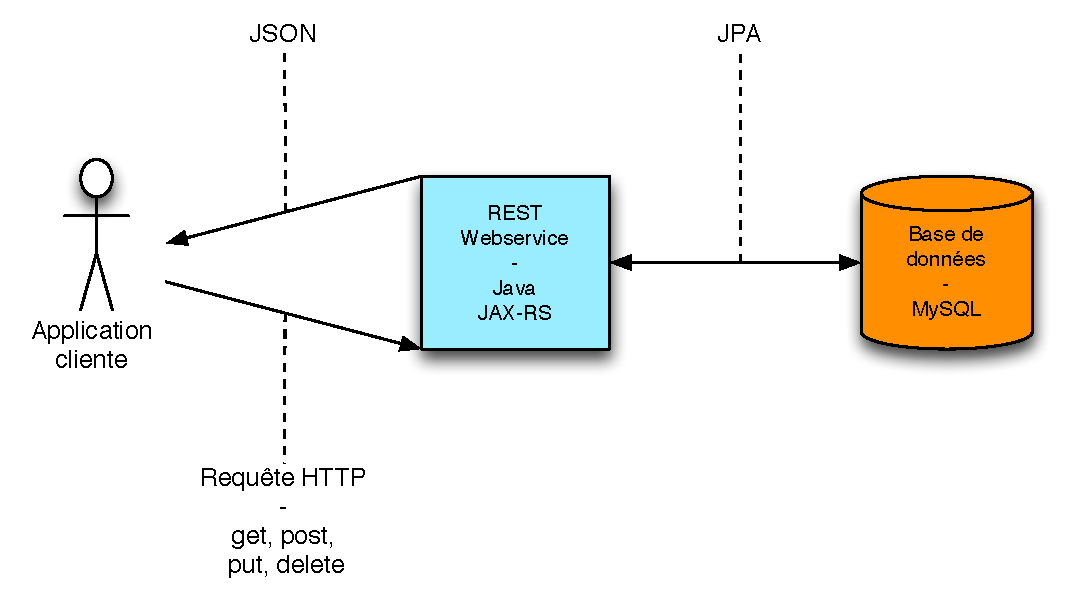
\includegraphics[width=14cm]{00_media/04_Serveur_archi.pdf}
      \caption{Architecture du serveur}
      \label{gra:archiServeur}
\end{figure}

L'application cliente requête le \emph{\gls{webservice}} à l'aire du protocole \emph{\gls{http}} et peut employer des types de méthodes comme \emph{get, post, put, delete}.

\medskip

L'application cliente reçoit les réponses au format \emph{\gls{json}} et se charge des les transformer selon ses besoins.

\medskip

Le \emph{\gls{webservice}} est de type \emph{\gls{rest}} et est implémenté avec \emph{\gls{jaxrs}} qui est une interface de programmation \emph{\gls{java}} permettant de créer des \emph{\glspl{webservice}}.

\medskip

Le tout s'articule autour d'une base de données \emph{\gls{mysql}} qui permet d'enregistrer les données en utilisant \emph{\gls{jpa}}.

\subsection{Architecture du webservice} % (fold)
\label{sub:architecture_du_webservice}
Pour expliquer l'architecture et la structure du \emph{\gls{webservice}}, je vais m'aider de la figure \ref{gra:gethouselistsequence} qui est un diagramme de séquence très simple destiné à pouvoir, au fil du voyage de la requête, détaillé le processus. 

\begin{figure}[H]
      \centering
      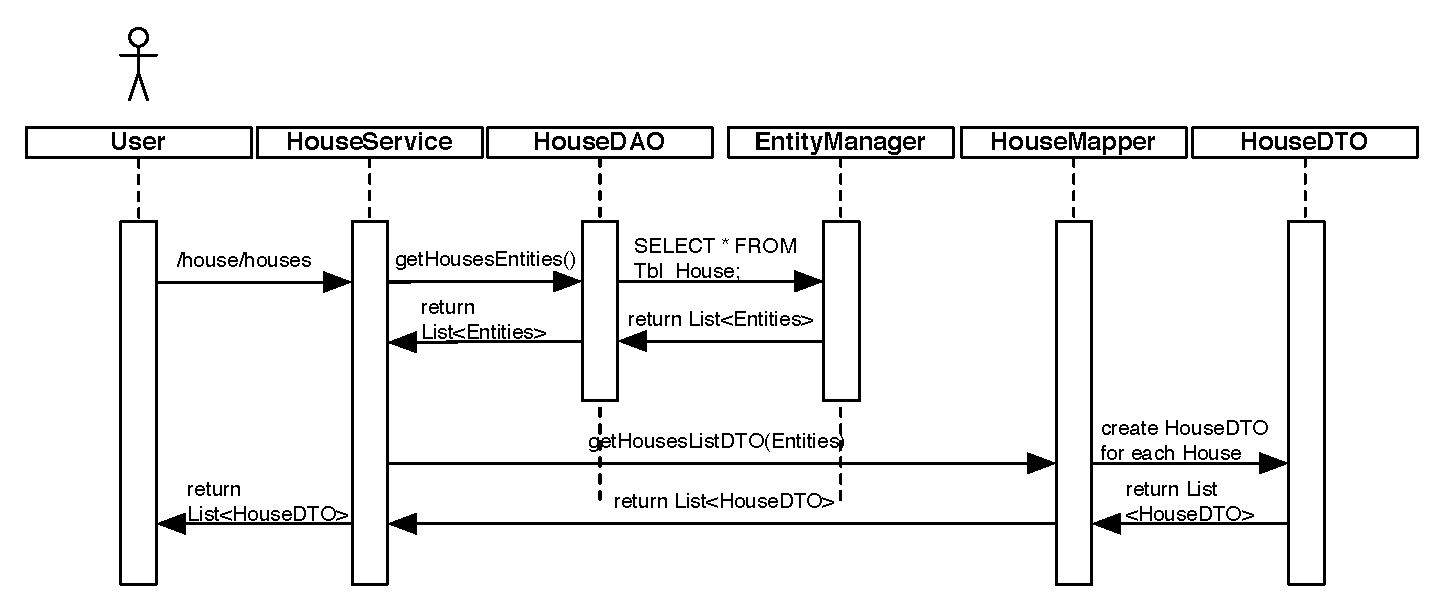
\includegraphics[width=\textwidth]{00_media/04_SequenceGetHousesList.pdf}
      \caption{Diargramme de séquence - GET Houses List}
      \label{gra:gethouselistsequence}
\end{figure}

L'utilisateur fait donc une requête sur le webservice à l'aide d'une fin d'\emph{\gls{url}} du type \emph{/house/houses}. La classe \texttt{HouseService} implémentée en \emph{\gls{jersey}} interroge la classe \texttt{HouseDAO} en lui demande de lui retourner toutes les entités. Elle attend donc une liste d'entités en retour. La classe \texttt{HouseDAO} se charge de sélectionner les entrées dans la base de données et les retournes sous formes de liste. Une fois la réponse arrivée à la classe \texttt{HouseService}, elle se charge de demander à la classe \texttt{HouseMapper} une liste qu'elle puisse retourner à l'utilisateur avec le bon format. La classe \texttt{HouseMapper} travaille avec \texttt{HouseDTO} qui permettra justement de faire ceci. Finalement, l'utilisateur reçoit sa réponse.

% subsection architecture_du_webservice (end)

\subsection{REST API pour l'application} % (fold)
\label{sub:rest_api_pour_l_application}
Cette section décrit l'interface (\emph{\gls{api}}) que doit fournir le \emph{\gls{webservice}} pour que toutes les opérations de l'application cliente soient possibles.

\medskip

L'\emph{\gls{api}} a été séparée en différentes parties afin de mieux cibler chacune d'elle, à savoir : 

\medskip

\begin{itemize}
	\item Login
	\item Maisons
	\item Zones
	\item Capteurs
	\item Données des capteurs
\end{itemize}

\medskip

Afin de rendre les tableaux qui suivent plus légers, toutes les \gls{url} doivent être précédées par \url{http://adresse:port/ga-service} pour fonctionner.

\subsubsection{Login}
Le tableau \ref{tab:apiLogin} permet de savoir comment utiliser le \emph{\gls{webservice}} pour recevoir et envoyer les informations de login.

\begin{table}[H]
\begin{tabularx}{\textwidth}{|X|X|X|X|X|}
  \hline
  \bf{Nom}  & \bf{URL} & \bf{Type} & \bf{Paramètres} & \bf{Retour} \\
  \hline  
  Se loguer  & /token/ask & GET &  user, password & Pas OK -> error 404 OK --> User \emph{\gls{json}}\\
  \hline  
  Contrôle login & /token/check & GET & token  & true, false\\
  \hline  
  Se délogguer & /token/logout & GET & token  & true, false\\
  \hline  
\end{tabularx}
\caption{API du webservice - Login}
\label{tab:apiLogin}
\end{table}

\subsubsection{Maisons}
Le tableau \ref{tab:apiMaison} permet de savoir comment utiliser le \emph{\gls{webservice}} pour recevoir et envoyer les informations sur les maisons.

\begin{table}[H]
\begin{tabularx}{\textwidth}{|X|m{3cm}|X|X|X|}
  \hline
  \bf{Nom}  & \bf{URL} & \bf{Type} & \bf{Paramètres} & \bf{Retour} \\
  \hline  
  Toutes les maisons  & /house/houses & GET &  - & Liste des maisons \emph{\gls{json}} \\
  \hline
 Les maisons d'un utilisateur  & /house/user/\{id\} & GET &  id & Liste des maisons \emph{\gls{json}} \\
  \hline 
 Créer une maison  & /house/create & POST & House \emph{\gls{json}} & House \emph{\gls{json}} \\
  \hline 
 Modifier une maison  & /house/update & POST & House \emph{\gls{json}} & House \emph{\gls{json}} \\
  \hline   
 Supprimer une maison  & /house/delete/\{id\} & DELETE &  id & error 404 ou 200 \\
  \hline  
\end{tabularx}
\caption{API du webservice - Maison}
\label{tab:apiMaison}
\end{table}

\subsubsection{Zones}
Le tableau \ref{tab:apiZone} permet de savoir comment utiliser le \emph{\gls{webservice}} pour recevoir et envoyer les informations sur les zones.

\begin{table}[H]
\begin{tabularx}{\textwidth}{|X|X|X|X|X|}
  \hline
  \bf{Nom}  & \bf{URL} & \bf{Type} & \bf{Paramètres} & \bf{Retour} \\
  \hline  
  Toutes les zones  & /zone/zones & GET &  - & Liste des zones \emph{\gls{json}} \\
  \hline
 Les zones d'une maison  & /zone/house/\{id\} & GET &  id & Liste des maisons \\
  \hline 
 Créer une zone  & /zone/save & POST & Zone \emph{\gls{json}} & Zone \emph{\gls{json}} \\
  \hline 
 Modifier une zone  & /zone/updateZone & POST & Zone \emph{\gls{json}} & Zone \emph{\gls{json}} \\
  \hline   
 Supprimer une zone  & /zone/delete/\{id\} & DELETE &  id & error 404 ou 200 \\
  \hline  
\end{tabularx}
\caption{API du webservice - Zone}
\label{tab:apiZone}
\end{table}

\subsubsection{Capteurs}
Le tableau \ref{tab:apiCapteur} permet de savoir comment utiliser le \emph{\gls{webservice}} pour recevoir et envoyer les informations sur les capteurs.

\begin{table}[H]
\begin{tabularx}{\textwidth}{|X|m{3cm}|X|X|X|}
  \hline
  \bf{Nom}  & \bf{URL} & \bf{Type} & \bf{Paramètres} & \bf{Retour} \\
  \hline  
  Tous les capteurs  & /sensor/sensors & GET &  - & Liste des capteurs \emph{\gls{json}} \\
  \hline
 Les capteurs d'une zone  & /sensor/zone/\{id\} & GET &  id & Liste des capteurs \\
  \hline 
 Modifier un capteur  & /sensor/update & PUT & Sensor \emph{\gls{json}} & Sensor \emph{\gls{json}} \\
  \hline   
   Retirer d'une zone & /sensor/noZone & POST &  Sensor \emph{\gls{json}} & Sensor \\
  \hline  
\end{tabularx}
\caption{API du webservice - Capteur}
\label{tab:apiCapteur}
\end{table}

\subsubsection{Données des capteurs}
Le tableau \ref{tab:apiCapteurData} permet de savoir comment utiliser le \emph{\gls{webservice}} pour recevoir les données des capteurs.

\begin{table}[H]
\begin{tabularx}{\textwidth}{|X|X|X|X|X|}
  \hline
  \bf{Nom}  & \bf{URL} & \bf{Type} & \bf{Paramètres} & \bf{Retour} \\
  \hline  
  Les données pour un capteur  & /sensorData/sensor/{id} & GET &  id & Liste des données \emph{\gls{json}} \\
  \hline
 Les dernières données pour un capteur  & /sensorData/sensor/\{id\}/last & GET & id & Liste des données \emph{\gls{json}} \\
  \hline 
\end{tabularx}
\caption{API du webservice - Données du capteur}
\label{tab:apiCapteurData}
\end{table}
% subsection rest_api_pour_l_application (end)
%	%!TEX root = ../rapport.tex

\section{Réalisation}
Cette section a pour but de présenter certains détails jugés importants par rapport à l'implémentation.

\medskip

Pour se faire, je vais expliqué chaque package qui mérite explications et qui a été modifiée pendant le projet. Voici pour commencer la liste des packages en question: 

\medskip

\begin{itemize}
	\item \emph{\gls{dao}} qui est le package d'interface vers la base de données
	\item \emph{\gls{dto}} qui permet de convertir un objet dans un format demandé par l'utilisateur
	\item \emph{Mapper} qui retourne des objets \emph{\gls{java}} correspondant aux entités \emph{\gls{jpa}} passées en paramètres
	\item \emph{Model} qui contient les entités \emph{\gls{jpa}}
	\item \emph{Resource} qui contient les ressources implémentées en \emph{\gls{jersey}}
\end{itemize}

\subsection{HouseDAO} % (fold)
\label{sub:housedao}
Cette classe contient donc des méthodes allant interroger la base de données. Typiquement, le code \ref{lst:serverdao} sélectionne la maison avec un certain id.
\begin{lstlisting}[language={JAVA}, caption={DAO - Maison avec id}, label={lst:serverdao}]
public Tbl_House getHouseById(int id) {
	
	EntityManager em = DBManager.getInstance().getNewEntityManager();
	try {
		TypedQuery<Tbl_House> q = em.createNamedQuery("House.findById", Tbl_House.class);
		q.setParameter("id", Long.valueOf(id));
		return q.getSingleResult();
	} finally {
		em.close();
	}

}
\end{lstlisting}

On utilise ci-dessus une requête nommée qui a été inséré directement dans la classe de l'entité concerné sous la forme du code \ref{lst:namedrequest}.

\begin{lstlisting}[language={JAVA}, caption={Requête nommée}, label={lst:namedrequest}]
@NamedQuery(name="House.findById", query="SELECT t FROM Tbl_House t where t.ho_PK_House = :id ")
\end{lstlisting}
% subsection housedao (end)
%	%!TEX root = ../rapport.tex

\section{Tests}

Pour ce qui est des tests de la partie serveur, j'ai pris chaque requête proposé par l'\emph{\gls{api}} et je l'ai envoyé avec \emph{WizTools.org RESTClient} qui me retourne une réponse bien lisible.
\subsection{Login} % (fold)
\label{sub:login}
Le tableau \ref{tab:stestLogin} reporte les résultats des tests qui ont été effectués pour la partie login de l'application.
\begin{table}[H]
\begin{tabularx}{\textwidth}{|X|X|X|X|}
  \hline
  \bf{Descriptif} & \bf{Paramètres} & \bf{Résultat attendu} & \bf{Résultat obtenu}\\
  \hline
   Se loguer & mot de passe faux & Erreur 404 & 
\includegraphics[width=16px]{00_media/ok.png} \\
  \hline
     Se loguer & utilisateur faux & Erreur 404 & 
\includegraphics[width=16px]{00_media/ok.png} \\
  \hline
       Se loguer & informations correctes & \emph{\gls{json}} user & 
\includegraphics[width=16px]{00_media/ok.png} \\
  \hline
\end{tabularx}
\caption{Tests - Serveur - Résultats des tests pour la partie login}
\label{tab:stestLogin}
\end{table}
% subsection login (end)
\subsection{Maisons} % (fold)
\label{sub:login}
Le tableau \ref{tab:stestMaison} reporte les résultats des tests qui ont été effectués pour la partie maison de l'application.
\begin{table}[H]
\begin{tabularx}{\textwidth}{|X|X|X|X|}
  \hline
  \bf{Descriptif} & \bf{Paramètres} & \bf{Résultat attendu} & \bf{Résultat obtenu}\\
  \hline
  Toutes les maisons & - & Liste des maisons \emph{\gls{json}} & 
\includegraphics[width=16px]{00_media/ok.png} \\
  \hline
  Les maisons d'un user & id correct & Liste des maisons \emph{\gls{json}} & 
\includegraphics[width=16px]{00_media/ok.png} \\
  \hline
  Les maisons d'un user & id incorrect & null & 
\includegraphics[width=16px]{00_media/ok.png} \\
  \hline
   Créer une maison & Maison \emph{\gls{json}} & Maison \emph{\gls{json}} & 
\includegraphics[width=16px]{00_media/ok.png} \\
  \hline
  Créer une maison & rien & Erreur & 
\includegraphics[width=16px]{00_media/ok.png} \\
  \hline
   Modifier une maison & rien & Erreur & 
\includegraphics[width=16px]{00_media/ok.png} \\
  \hline
  Modifier une maison & Modification sur une maison & Maison \emph{\gls{json}} & 
\includegraphics[width=16px]{00_media/ok.png} \\
  \hline
  Modifier une maison & maison qui n'existe pas & Erreur & 
\includegraphics[width=16px]{00_media/ok.png} \\
  \hline
  Supprimer une maison & id correct & 204 ok & 
\includegraphics[width=16px]{00_media/ok.png} \\
  \hline
   Supprimer une maison & id incorrect & 404 & 
\includegraphics[width=16px]{00_media/ok.png} \\
  \hline
\end{tabularx}
\caption{Tests - Serveur - Résultats des tests pour la partie maison}
\label{tab:stestMaison}
\end{table}

\clearpage

\subsection{Zones} % (fold)
\label{sub:login}
Le tableau \ref{tab:stestZone} reporte les résultats des tests qui ont été effectués pour la partie zone de l'application.
\begin{table}[H]
\begin{tabularx}{\textwidth}{|X|X|X|X|}
  \hline
  \bf{Descriptif} & \bf{Paramètres} & \bf{Résultat attendu} & \bf{Résultat obtenu}\\
  \hline
  Toutes les zones & - & Liste des zones \emph{\gls{json}} & 
\includegraphics[width=16px]{00_media/ok.png} \\
  \hline
  Les zones d'une maison & id correct & Liste des zones \emph{\gls{json}} & 
\includegraphics[width=16px]{00_media/ok.png} \\
  \hline
  Les zones d'une maison & id incorrect & null  & 
\includegraphics[width=16px]{00_media/ok.png} \\
  \hline  
 Créer une zone & zone correcte & zone \emph{\gls{json}} & 
\includegraphics[width=16px]{00_media/ok.png} \\
  \hline 
  Créer une zone & pas de zone & erreur & 
\includegraphics[width=16px]{00_media/ok.png} \\
  \hline 
  Créer une zone & zone déjà existante & erreur & 
\includegraphics[width=16px]{00_media/ok.png} \\
  \hline 
  Modifier une zone & zone déjà existante & zone \emph{\gls{json}} & 
\includegraphics[width=16px]{00_media/ok.png} \\
  \hline
  Modifier une zone & zone inexistante & zone \emph{\gls{json}} & 
\includegraphics[width=16px]{00_media/ok.png} \\
  \hline
  Supprimer une zone & zone inexistante & erreur 404  & 
\includegraphics[width=16px]{00_media/ok.png} \\
  \hline
  Supprimer une zone & zone existante & 204 & \includegraphics[width=16px]{00_media/ok.png} \\
  \hline
\end{tabularx}
\caption{Tests - Serveur - Résultats des tests pour la partie zone}
\label{tab:stestZone}
\end{table}

\clearpage

\subsection{Capteurs} % (fold)
\label{sub:login}
Le tableau \ref{tab:stestSensor} reporte les résultats des tests qui ont été effectués pour la partie capteur de l'application.
\begin{table}[H]
\begin{tabularx}{\textwidth}{|X|X|X|X|}
  \hline
  \bf{Descriptif} & \bf{Paramètres} & \bf{Résultat attendu} & \bf{Résultat obtenu}\\
  \hline
  Toutes les capteurs & - & Liste des capteurs \emph{\gls{json}} & \includegraphics[width=16px]{00_media/ok.png} \\
  \hline
  Les capteurs d'une zone & id correct & Liste des capteurs \emph{\gls{json}} & \includegraphics[width=16px]{00_media/ok.png} \\
  \hline
  Les capteurs d'une zone & id incorrect & null & \includegraphics[width=16px]{00_media/ok.png} \\
  \hline
  Modifier un capteur & - & erreur 404 & \includegraphics[width=16px]{00_media/ok.png} \\
  \hline
  Modifier un capteur & nouveau capteur & null & \includegraphics[width=16px]{00_media/ok.png} \\
  \hline
  Modifier un capteur & Capteur existant & Capteur \emph{\gls{json}} & \includegraphics[width=16px]{00_media/ok.png} \\
  \hline
  Supprimer un capteur d'une zone & Capteur existant & Capteur \emph{\gls{json}} & \includegraphics[width=16px]{00_media/ok.png} \\
  \hline
  Supprimer un capteur d'une zone & Capteur inexistant & null & \includegraphics[width=16px]{00_media/ok.png} \\
  \hline
  Supprimer un capteur d'une zone & Capteur pas dans la zone & Capteur \emph{\gls{json}} & \includegraphics[width=16px]{00_media/ok.png} \\
  \hline
\end{tabularx}
\caption{Tests - Serveur - Résultats des tests pour la partie capteur}
\label{tab:stestSensor}
\end{table}

\clearpage

\subsection{Données du capteur} % (fold)
\label{sub:login}
Le tableau \ref{tab:stestData} reporte les résultats des tests qui ont été effectués pour la partie données du capteur de l'application.
\begin{table}[H]
\begin{tabularx}{\textwidth}{|X|X|X|X|}
  \hline
  \bf{Descriptif} & \bf{Paramètres} & \bf{Résultat attendu} & \bf{Résultat obtenu}\\
  \hline
  Les données pour un capteur & capteur existant & données \emph{\gls{json}} & \includegraphics[width=16px]{00_media/ok.png} \\
  \hline
  Les données pour un capteur & capteur inexistant & null & \includegraphics[width=16px]{00_media/ok.png} \\
  \hline
  Les dernières données pour un capteur & capteur existant & données \emph{\gls{json}} & \includegraphics[width=16px]{00_media/ok.png} \\
  \hline
  Les dernières données pour un capteur & capteur inexistant & null & \includegraphics[width=16px]{00_media/ok.png} \\
  \hline
\end{tabularx}
\caption{Tests - Serveur - Résultats des tests pour la partie données du capteur}
\label{tab:stestData}
\end{table}
%
%	%!TEX root = ../rapport.tex


\chapter{Tests sur l'ensemble du projet}
\label{testensembleprojet}
\begin{epigraphs}
\qitem{Program testing can be used to show the presence of bugs, but never to show their absence!}%
{---\textsc{Edsger W. Dijkstra}}
\end{epigraphs}

Ce chapitre reporte les résultats obtenus lors de différents tests effectués sur l'application. Tout d'abord, des tests fonctionnels ont été organisés pour prendre connaissance des éventuels problèmes. Ensuite, des personnes volontaires ont consacré un peu de temps pour "jouer" avec l'application et je reporte ici les principales remarques citées lors de cette expérience.

\section{Tests fonctionnels} % (fold)
\label{sec:tests_fonctionnels}

\subsection{Login} % (fold)
\label{sub:login}
Le tableau \ref{tab:testLogin} reporte les résultats des tests qui ont été effectués pour la partie login de l'application.
\begin{table}[H]
\begin{tabularx}{\textwidth}{|X|X|m{1.5cm}|}
  \hline
  \bf{Descriptif} & \bf{Résultat attendu} & \bf{Résultat obtenu} \\
  \hline
  Le serveur n'est pas atteignable et l'utilisateur se loggue & Message d'information & \includegraphics[width=16px]{00_media/ok.png} \\
  \hline
  Le serveur est atteignable et l'utilisateur se loggue avec des paramètres non valides & Message d'information & \includegraphics[width=16px]{00_media/ok.png} \\
  \hline
    Le serveur est atteignable et l'utilisateur se loggue avec des paramètres valides & L'application change de vue & \includegraphics[width=16px]{00_media/ok.png} \\
  \hline
\end{tabularx}
\caption{Tests - Résultats des tests pour la partie login}
\label{tab:testLogin}
\end{table}
% subsection authentification (end)

\subsection{Logout} % (fold)
\label{sub:logout}
Le tableau \ref{tab:testLogout} reporte les résultats des tests qui ont été effectués pour la partie logout de l'application.
\begin{table}[H]
\begin{tabularx}{\textwidth}{|X|X|m{1.5cm}|}
  \hline
  \bf{Descriptif} & \bf{Résultat attendu} & \bf{Résultat obtenu} \\
  \hline
  Le serveur n'est pas atteignable et l'utilisateur se déloggue & L'application change de vue & \includegraphics[width=16px]{00_media/ok.png} \\
  \hline
  Le serveur est atteignable et l'utilisateur se déloggue  & L'application change de vue & \includegraphics[width=16px]{00_media/ok.png} \\
  \hline
\end{tabularx}
\caption{Tests - Résultats des tests pour la partie logout}
\label{tab:testLogout}
\end{table}
% subsection logout (end)

\subsection{Liste des maisons} % (fold)
\label{sub:logout}
Le tableau \ref{tab:testListMaison} reporte les résultats des tests qui ont été effectués lors de l'affichage de la liste des maisons.
\begin{table}[H]
\begin{tabularx}{\textwidth}{|X|X|m{1.5cm}|}
  \hline
  \bf{Descriptif} & \bf{Résultat attendu} & \bf{Résultat obtenu} \\
  \hline
  L'utilisateur affiche la liste des maisons&La liste s'affiche correctement & \includegraphics[width=16px]{00_media/ok.png} \\
  \hline
  L'utilisateur affiche la liste des maisons et le serveur n'est pas accessible & La liste s'affiche correctement & \includegraphics[width=16px]{00_media/ok.png} \\
\hline
  L'utilisateur filtre les résultats en utilisant le champ de recherche & La liste s'affiche et prend en compte l'entrée de l'utilisateur & \includegraphics[width=16px]{00_media/ok.png} \\
  \hline
    L'utilisateur filtre les résultats en utilisant le champ de recherche et le serveur n'est pas accessible & La liste s'affiche et prend en compte l'entrée de l'utilisateur & \includegraphics[width=16px]{00_media/ok.png} \\
  \hline
    L'utilisateur clique sur une maison & La maison s'affiche correctement & \includegraphics[width=16px]{00_media/ok.png} \\
  \hline
      L'utilisateur clique sur une maison et le serveur n'est pas accessible & Message d'informations concernant le problème & \includegraphics[width=16px]{00_media/ok.png} \\
  \hline
\end{tabularx}
\caption{Tests - Résultats des tests pour la partie liste de maisons}
\label{tab:testListMaison}
\end{table}
% subsection logout (end)

\clearpage

\subsection{Affichage du plan} % (fold)
\label{sub:logout}
Le tableau \ref{tab:testAffichagePlan} reporte les résultats des tests qui ont été effectués lors de l'affichage du plan.
\begin{table}[H]
\begin{tabularx}{\textwidth}{|X|X|m{1.5cm}|}
  \hline
  \bf{Descriptif} & \bf{Résultat attendu} & \bf{Résultat obtenu} \\
  \hline
  Le plan existe dans dans la librairie & L'image s'affiche & \includegraphics[width=16px]{00_media/ok.png} \\
  \hline
  Le plan n'existe  pas dans la librairie & Message d'information & \includegraphics[width=16px]{00_media/ok.png} \\
  \hline

\end{tabularx}
\caption{Tests - Résultats des tests pour la partie de l'affichage du plan}
\label{tab:testAffichagePlan}
\end{table}
% subsection logout (end)

\subsection{Affichage des zones} % (fold)
\label{sub:logout}
Le tableau \ref{tab:testAffichageZones} reporte les résultats des tests qui ont été effectués lors de l'affichage des zones.
\begin{table}[H]
\begin{tabularx}{\textwidth}{|X|X|m{1.5cm}|}
  \hline
  \bf{Descriptif} & \bf{Résultat attendu} & \bf{Résultat obtenu} \\
  \hline
  La maison comporte une ou des zones & La ou les zones sont affichées sur le plan & \includegraphics[width=16px]{00_media/ok.png} \\
  \hline
  La maison ne comporte aucune zone & Le plan est affiché normalement sans zones & \includegraphics[width=16px]{00_media/ok.png} \\
  \hline
  La maison comporte des zones qui n'ont pas de paramètres d'affichage (taille, position)& Les zones sont affichées tout en haut à gauche du plan & \includegraphics[width=16px]{00_media/ok.png} \\
  \hline
\end{tabularx}
\caption{Tests - Résultats des tests pour la partie de l'affichage des zones}
\label{tab:testAffichageZones}
\end{table}

\subsection{Modification des zones} % (fold)
\label{sub:logout}
Le tableau \ref{tab:testAffichageZones} reporte les résultats des tests qui ont été effectués lors du déplacement, l'agrandissement et la rotation des zones sur le plan.
\begin{table}[H]
\begin{tabularx}{\textwidth}{|X|X|m{1.5cm}|}
  \hline
  \bf{Descriptif} & \bf{Résultat attendu} & \bf{Résultat obtenu} \\
  \hline
  L'utilisateur déplace une zone  & La zone se déplace mais ne sort pas du plan & \includegraphics[width=16px]{00_media/ok.png} \\
  \hline
  L'utilisateur modifie la taille une zone  & La zone agrandit ou diminue sa taille  & \includegraphics[width=16px]{00_media/ok.png} \\
  \hline
  L'utilisateur tourne une zone  & La zone se tourne  & \includegraphics[width=16px]{00_media/ok.png} \\
  \hline
  L'utilisateur déplace une zone après l'avoir agrandi & Mouvement normal & \includegraphics[width=16px]{00_media/not_ok.png} \\
  \hline
\end{tabularx}
\caption{Tests - Résultats des tests pour la partie de la modification des zones}
\label{tab:testAffichageZones}
\end{table}
Il y a effectivement encore un bug avec le mouvement ou la rotation des zones après un agrandissement. 
% subsection logout (end)
% section tests_fonctionnels (end)

\section{Expériences utilisateurs} % (fold)
\label{sec:exp_riences_utilisateurs}
J'ai à plusieurs reprises demandé à des connaissances de tester mon application. Ce qu'il en est principalement ressorti est un point que j'avais déjà soulevé concernant le bug de déplacement des zones après un agrandissement.

\medskip

Il y aussi le fait que certaines personnes ne savaient pas trop quand il fallait enregistrer, si cela était fait automatiquement, etc ..

\medskip

D'une manière général, ils ont compris assez vite le fonctionnement de l'application et ont même trouvé cela assez intuitif.

\medskip

Au niveau du design, il est ressorti que les couleurs étaient bien choisies car elles mettaient en confiance l'utilisateur.
% section exp_riences_utilisateurs (end)
%
%	%!TEX root = ../rapport.tex

\chapter{Résultats} % (fold)
\label{cha:r_sultats}
Ce chapitre a pour but d'illustrer les résultats obtenus sur l'\emph{\gls{ipad}} par des maquettes qui sont tirées de l'application finale. Ce chapitre peut également servir de guide pour un utilisateur voulant utiliser l'application.

\section{Icône} % (fold)
\label{sec:ic_ne}
La figure \ref{gra:res01} montre l'îcone de l'application \emph{iGreenControl}. L'utilisateur presse sur cette îcone pour lancer l'application.
\begin{figure}[H]
     	\centering
     	\includegraphics[width=14cm]{00_media/07_01.PNG}
     	\caption{Résultats - Icône}
     	\label{gra:res01}
 \end{figure} 
% section ic_ne (end)

\clearpage

\section{Login} % (fold)
\label{sec:login}
La figure \ref{gra:res02} illustre ce que voit l'utilisateur quand il lance l'application, il peut alors entrer ses informations d'authentification.
\begin{figure}[H]
     	\centering
     	\includegraphics[width=\textwidth]{00_media/07_02.PNG}
     	\caption{Résultats - Ecran de login}
     	\label{gra:res02}
 \end{figure} 

\clearpage

\section{Informations} % (fold)
\label{sec:informations}
La figure \ref{gra:res03} résulte de la partie \emph{Infos} de l'application lorsque l'utilisateur clique sur le bouton correspondant.
\begin{figure}[H]
     	\centering
     	\includegraphics[width=\textwidth]{00_media/07_03.PNG}
     	\caption{Résultats - Informations}
     	\label{gra:res03}
 \end{figure} 

\clearpage


\section{Menu maison} % (fold)
\label{sec:menu_maisons}
La figure \ref{gra:res04} montre le menu qui apparait lorsque l'utilisateur clique sur le bouton \emph{Maison}. 

\begin{figure}[H]
    	\centering
    	\includegraphics[width=\textwidth]{00_media/07_04.PNG}
    	\caption{Résultats - Menu maison}
    	\label{gra:res04}
\end{figure}

\clearpage


\section{Liste des maisons} % (fold)
\label{sub:liste_des_maisons}
Lorsque l'utilisateur clique sur la liste des maisons, il voit assez logiquement la liste des maisons qui lui appartiennent comme le montre la figure \ref{gra:res05}. Il peut alors soit cliquer sur une maison pour l'ouvrir, soit faire un défilement de gauche à droite avec le doigt pour afficher le bouton de suppression.
\begin{figure}[H]
        \centering
        \includegraphics[width=\textwidth]{00_media/07_05.PNG}
        \caption{Résultats - Liste des maisons}
        \label{gra:res05}
\end{figure}
% subsection liste_des_maisons (end)

\clearpage


\section{Nouvelle maison} % (fold)
\label{sub:nouvelle_maison}
Lorsque l'utilisateur veut créer une nouvelle maison, il peut apercevoir un écran comme sur la figure \ref{gra:res06}. Il a la possibilité de remplir les informations et de créer la maison.
\begin{figure}[H]
        \centering
        \includegraphics[width=\textwidth]{00_media/07_06.PNG}
        \caption{Résultats - Créer une nouvelle maison}
        \label{gra:res06}
\end{figure}

\clearpage


\section{Sélectionner une image} % (fold)
\label{sub:s_lectionner_une_image}
La figure \ref{gra:res07} montre l'explorateur d'image quand l'utilisateur veut importer un plan. Dès qu'une image est sélectionnée, celle-ci s'affiche dans l'application.
\begin{figure}[H]
        \centering
        \includegraphics[width=\textwidth]{00_media/07_07.PNG}
        \caption{Résultats - Sélectionner une photo}
        \label{gra:res07}
\end{figure}

% subsection s_lectionner_une_image (end)

\clearpage


\section{Insertion d'une zone} % (fold)
\label{sub:insertion_d_une_zone}
La figure \ref{gra:res08} montre l'écran que voit l'utilisateur lorsqu'il désire insérer une nouvelle zone dans le plan. Il peut alors insérer les informations sur la zone et la créer en cliquand sur le bouton.
% subsection insertion_d_une_zone (end)
\begin{figure}[H]
        \centering
        \includegraphics[width=\textwidth]{00_media/07_08.PNG}
        \caption{Résultats - Créer une nouvelle zone}
        \label{gra:res08}
\end{figure}

\clearpage


\section{Affichage d'un plan} % (fold)
\label{sub:subsection_ame}
Lorsque l'utilisateur ouvre une maison qui est déjà configurée et qui contient des zones et des capteurs, il peut par exemple voir un résultat comme sur la figure \ref{gra:res09}.

\medskip

Les opérations possibles pour le plan sont : 

\medskip

\begin{itemize}
    \item Redimensionner le plan (cela redimensionne également les éléments qui sont à l'intérieur du plan)
    \item Déplacer le plan (cela déplace également les éléments qui sont à l'intérieur du plan)
\end{itemize}

\medskip

Les opérations disponibles sur les zones sont : 

\medskip

\begin{itemize}
    \item Redimensionner uniquement les zones
    \item Déplacer les zones (cela déplace également les éventuels capteurs qui sont à l'intérieur)
    \item Faire pivoter les zones
    \item Presser un certain temps sur la zone afin d'afficher un menu spécifique à la zone
\end{itemize}

% subsection subsection_name (end)
\begin{figure}[H]
        \centering
        \includegraphics[width=\textwidth]{00_media/07_09.PNG}
        \caption{Résultats - Plan affiché}
        \label{gra:res09}
\end{figure}

\clearpage

\section{Paramètres d'une zone} % (fold)
\label{sub:param_tres_d_une_zone}
La figure \ref{gra:res10} montre le menu qui est présenté à l'utilisateur lorsque ce dernier presse un certain temps sur une zone. Il peut alors modifier les paramètres de la zone ou la supprimer.

\begin{figure}[H]
        \centering
        \includegraphics[width=\textwidth]{00_media/07_10.PNG}
        \caption{Résultats - Paramètres d'une zone}
        \label{gra:res10}
\end{figure}

\clearpage


\section{Insertion d'un capteur} % (fold)
\label{sub:insertion_d_un_capteur}

Toujours en pressant un certain temps sur une zone, l'utilisateur à la possibilité d'insérer un capteur. Une liste de capteurs disponible lui est alors présenté et il peut alors en sélectionner un dans le but de le relier à la zone. La liste des capteurs peut être aperçue à la figure \ref{gra:res11}.

\begin{figure}[H]
        \centering
        \includegraphics[width=\textwidth]{00_media/07_11.PNG}
        \caption{Résultats - Insertion d'un nouveau capteur}
        \label{gra:res11}
\end{figure}

\clearpage


\section{Paramètres d'un capteur} % (fold)
\label{sec:param_tres_d_un_capteur}
Lorsqu'il clique un certain temps sur un capteur, l'utilisateur voit apparaître un menu pour le capteur. Sur la figure \ref{gra:res12}, vous pouvez voir comment on peut modifier ou supprimer un capteur.

\begin{figure}[H]
        \centering
        \includegraphics[width=\textwidth]{00_media/07_12.PNG}
        \caption{Résultats - Paramètres d'un capteur}
        \label{gra:res12}
\end{figure}

\clearpage


\section{Données d'un capteur} % (fold)
\label{sec:donn_es_d_un_capteur}
Sur la figure \ref{gra:res13}, ce sont les données du capteurs qui peuvent être distinguées. L'utilisateur peut alors les rafraîchir dès qu'il le souhaite.
% section donn_es_d_un_capteur (end)
\begin{figure}[H]
        \centering
        \includegraphics[width=\textwidth]{00_media/07_13.PNG}
        \caption{Résultats - Visualiser les données d'un capteur}
        \label{gra:res13}
\end{figure}
% subsection nouvelle_maison (end)
% section menu_maisons (end)

% section informations (end)
% chapter r_sultats (end)
%	
%	%!TEX root = ../rapport.tex

\chapter{Conclusion} % (fold)
\label{cha:conclusion}
Voici le chapitre final, concluant ce travail de Bachelor. Je vais vous donner mes impressions personnelles, les problèmes rencontrer ainsi que les amélioration possibles de l'application.


\section{Impressions personnelles} % (fold)
\label{sec:impression_personnelle}
J'ai énormément aimé travailler sur ce projet et j'ai beaucoup appris.

\medskip

Techniquement, j'ai pu découvrir énormément: l'utilisation des qualités de services dans une application, la communication à travers les WebSockets, la mise en place d'un serveur avec les Web Services. Bien que ce n'était pas une application Android la plus complète que l'on puisse faire, sans interface graphique, j'ai tout de même bien pu mettre en pratique les notions du développement sur ce système d'exploitation.

\medskip

J'ai aussi pu réutiliser du Backbone pour la partie Web, bien qu'un tout petit peu, mais j'avais justement eu l'occasion d'en faire durant un projet de semestre et j'étais content de voir que je connaissais cette technologie, et que je n'ai pas été dépaysé lorsque j'ai dû la réutiliser!

\medskip

Pour l'expérience en soit, j'ai été ravi de découvrir une entreprise telle que Wingo. J'ai vraiment été très bien accueilli et supporté tout le long du projet. Je remercie grandement Olivier qui a été mon responsable durant ce projet, ainsi que toute l'équipe avec qui je me suis bien entendu. J'ai d'ailleurs profiter des petits plaisirs en entreprise comme une petite journée sportive avec tout le monde!

\medskip

C'était vraiment très intéressant et enrichissant, je recommande à tout le monde d'essayer!

\medskip

Je remercie aussi Jean-Frédéric Wagen, Jean-Roland Schuler et Benoît Piller, avec qui les discussions durant les séances hebdomadaires se sont toujours bien déroulées et ont été constructives.

\medskip

J'ai beaucoup redouté de commencer ce projet, car je ne savais pas chez qui j'allais atterrir et que la partie réseau des qualités de service me faisait un peu peur. Mais finalement tout s'est très bien déroulé et je ne regrette pas une seule seconde le choix que j'ai fait. Rarement un projet n'a été aussi passionnant du début à la fin

\medskip

Par contre mes vieux défauts sont toujours là, notamment au niveau de la documentation que je n'ai pas tenu à jour durant toute la durée du projet. J'ai malheureusement quelques parties manquantes, notamment au niveau des résultats qui manquent ainsi que de l'analyse. Mais je sais que j'ai de quoi être fier du projet en soit, et que le travail est là.

\medskip

Je suis par contre un peu déçu d'avoir finalement perdu du temps sur la partie du serveur, avec la gestion de la connexion et la connexion sécurisée, car quasiment tout le projet s'est déroulé sans encombre et dans les temps. Par contre dès qu'un peu de retard a été pris il a été difficile de le rattraper, surtout lorsque cela arrive sur la fin. J'ai pour le coup dû mettre de côté la phase finale des tests, ce qui est très dommage car j'aurais pu apprendre encore beaucoup!
\section{Problèmes rencontrés} % (fold)
\label{sec:probl_mes_rencontr_s}

\subsection{Déploiement sur la Set-Top Box} % (fold)
Le déploiement ne fonctionnait au début pas sur la box, alors qu'il fonctionnait sur la tablette. C'est Robert, développeur chez Swisscom, qui m'a dit de ne pas passer par Eclipse mais de le faire manuellement avec adb.
% subsection insertion_des_capteurs (end)

\subsection{Installation de Jersey sur Jetty} % (fold)
L'installation m'a donné du fil à retordre à cause de compatibilité de versions. J'aurais dû mieux lire la documentation dès le départ, ce qui m'aurait préserver quelques heures d'arrachage de cheveux!

\subsection{Mise en place de SSL}
A cause apparemment d'un bug dans la version 9.0.3 de Jetty corrigé dans la 9.0.4 puis du fait que Autobahn Android ne faisait confiance à tous les certificats qu'en étant dans le simulateur d'ADB, j'ai perdu un précieux temps sur la fin du projet.


\section{Améliorations} % (fold)
\label{sec:am_liorations}
\subsection{Récupérer automatiquement les qualités de services} % (fold)
Lorsque l'on arrive sur Thom, nous pourrions dynamiquement afficher les commandes que l'on peut envoyer sur notre STB, et non l'ajouter manuellement comme c'est le cas à présent.
% subsection dessiner_sa_maison (end)
\subsection{Améliorer l'ergonomie de l'application} % (fold)
Ce qui a été implémenté sur Thom est très basique. Aucune vérification n'est faite, très peu de retour pour l'utilisateur et peu de gestion d'erreurs.
% subsection cat_gorie_d_un_capteur (end)

\subsection{Voir la reconnexion d'une STB après reboot} % (fold)
Lorsque l'on redémarre à distance une box, nous n'avons pas de suivi. Cela veut dire que nous ne savons pas vraiment si tout s'est bien passé ou non. Il serait envisageable de pouvoir retourner lorsque la box est à nouveau connectée sur le serveur.
% subsection actuateur (end)

\subsection{Ajout de commandes à distance} % (fold)
Plus qu'une simple analyse des qualités de service, c'est vraiment une prise en main à distance qui est possible. On l'a vu notamment avec le reboot. Ce n'est pas une qualité mais c'est utile de pouvoir le faire à distance. Tout un tas de possibilités s'offrent à nous pour le dépannage.
% subsection version_iphone (end)


% section am_eliorations (end)

% chapter conclusion (end)


%	%!TEX root = ../rapport.tex

\chapter*{Remerciements}
\addcontentsline{toc}{chapter}{Remerciements}
Je souhaite remercier sincèrement toutes les personnes qui ont consacré du temps pour m'aider à réaliser ce projet.

\medskip

\begin{itemize}

	\item \textbf{Gérôme Bovet}, collaborateur scientifique à l'\emph{\gls{eiafr}} et responsable du projet de Bachelor, pour son suivi, ses conseils et les feedbacks apportés durant tout le projet.
	\medskip
	\item \textbf{Jean Hennebert} et \textbf{Omar Abou Khaled}, professeur à l'\emph{\gls{eiafr}} et superviseur du projet de Bachelor, pour leurs conseils et les feedback apportés durant tout le projet.
	\medskip
	\item \textbf{Giovanni Celato, Jean-Pascal Breu, Philippe Barras}, experts du projet, pour leurs conseils durant le projet.
	\medskip
	\item \textbf{Damien Vionnet}, collaborateur scientifique à l'\emph{\gls{eiafr}}, pour son aide concernant les licences et les certificats Apple permettant de déployer les applications sur un appareil \emph{\gls{ios}}.
	\medskip
	\item \textbf{Valentin Bourqui}, étudiant à l'\emph{\gls{eiafr}}, pour sa bonne collaboration durant le travail sur le \emph{\gls{webservice}}.
	\medskip
	\item \textbf{Laura Valenzano}, amie, pour la lecture de ce rapport et les conseils apportés.
	\medskip
	\item \textbf{Raphaël Morand, Olivier Perler, Clarisse Hernikat}, amis, pour avoir tester l'application finale et donner leur feedback.
	\medskip
	\item Et pour finir, \textbf{toutes les personnes} qui m'ont permis d'avancer au mieux en m'apportant leur confiance et leur soutien.

\end{itemize}
	
	%!TEX root = ../rapport.tex

\chapter{Introduction}
Ce chapitre introduit le cahier des charges du projet de Bachelor de l'eia-fr en informatique. Le projet se déroule avec la société WinGo S.A situé à Fribourg. WinGo est une filiale de Swisscom et propose des offres pour la télévision, Internet ainsi que la téléphonie sous le label "M-Budget".

La totalité du projet se déroulera dans leurs locaux situés à L'Avenue Beauregard 10 à Fribourg.

% section structure_du_document (end)
	%!TEX root = ../rapport.tex

\chapter{Contexte}

Comme dit précédemment, WinGo offre un service de TV sur Ip (IPTV). Il s'agit d'une Set-Top Box (STB) tournant sous Android qui reçoit le flux de données. Il est actuellement possible de mesurer la Qualité de Service (QoS) entre la plateforme de streaming IPTV et le routeur ADSL du client. Il n'est par contre pas possible de mesurer cette qualité entre le routeur et la STB. Le problème étant les différentes possibilités de connexions entre ces deux éléments, que cela soit par Ethernet ou par Wifi. Le but du projet est donc le développement d'une solution client (STB) - serveur (WinGo) permettant de mesurer la QoS.

\begin{figure}[H]
    \begin{center}
        \centering \includegraphics[width=0.7\linewidth]{CDC/schema_comm.png}
        \caption{Schéma de production actuel}
    \end{center}
\end{figure}

Voici l'environnement actuel en production, avec l'ajout d'un nouveau serveur.
\begin{itemize}
	\item Head End: C'est ici que les chaînes de TV sont reçues, encodées, encryptées et envoyées
	\item Thom: service de supervision. C'est ici que sont reportés tous les problèmes reportés avec leurs étapes de résolution.
	\item Serveur: C'est ici que l'implémentation côté serveur sera déployée
	\item Partie cliente: Routeur du client, connexion avec la STB qui contient le code Android permettant la communication avec notre nouveau serveur.
\end{itemize}

\medskip

La STB utilisée par WinGo est une box tournant sous Android. Il s'agit d'une surcouche graphique se superposant à l'image de la TV, donnant des informations supplémentaires comme la durée restante du programme en cours, le programme par chaînes etc. Il n'est pour le moment pas sûr que la box soit modifiable comme on le souhaite. C'est pourquoi dans un premier temps nous utiliserons un device tournant sous Android, à savoir une tablette Nexus 7 de Asus.
% section structure_du_document (end)
	%!TEX root = ../rapport.tex

\chapter{Objectifs}

\section{Primaires}
\begin{itemize}
	\item Analyse de produits existant permettant de définir la qualité d'un service
	\item Analyse sur la possibilité d'intégrer ces produits sur la STB de WinGo
	\item Implémentation d'un serveur recevant les données de la STB
	\item Implémentation de la STB sous Android
	\item Intégration des résultats du serveur sur la plateforme de supervision de l'entreprise
\end{itemize}

\section{Secondaires}
\begin{itemize}
	\item Implémentation d'une petite interface utilisateur affichant les résultats
\end{itemize}






% section structure_du_document (end)
%	%!TEX root = ../rapport.tex

\chapter{Spécifications}
La partie cliente est la Set-Top Box (STB). Celle-ci tourne sur Android et fait partie du réseau local de l'utilisateur. Il n'est pas possible d'atteindre directement un appareil depuis l'extérieur à cause des différentes couches de NAT. Il faudra donc que l'application soit la plus autonome possible. 

\medskip

Le lancement se fera donc au démarrage de la STB. Elle ne contiendra aucune interface graphique et n'aura aucun launcher. Le tout se fera sous la forme d'un service. Cela veut dire que tout se fera en "background".

\medskip

C'est l'application qui se chargera de se connecter au serveur. La connexion sera permanente, car nous n'aurons pas la possibilité de lancer le service à distance. Il faut donc qu'en cas de perte de connexion, une reconnexion soit faite automatiquement.

\medskip

Ensuite c'est elle aussi qui évaluera sa qualité de service. Les informations seront récoltées, puis envoyées au serveur. Elle devra juger la ligne qui se trouve entre la STB et le routeur.

\medskip

Pour la partie serveur, nous devons supporter une connexion permanente avec plusieurs centaines voir milliers d'appareils dans le futur. Le serveur devra récupérer les informations générées par la STB et les envoyer à un service de supervision, nommé THOM, qui lui affichera de manière lisible pour l'humain les résultats récoltés.

\medskip

Pour résumer, voici les spécifications:

\medskip

\begin{itemize}
	\item Service Android sans interface graphique ni launcher
	\item Lancement automatique au démarrage de la Set-Top Box
	\item Connexion au serveur grâce au service Android
	\item Récolte d'informations sur la qualité de service depuis la Set-Top Box entre celle-ci et le routeur.
	\item Transmission des données au serveur
	\item Serveur supportant des connexions permanentes la plus fiable possible
	\item Scalabilité permettant la connexion de multiples appareils
	\item Récolte des informations et transmission de celles-ci à un service de supervision
\end{itemize}


% section structure_du_document (end)
	%!TEX root = ../rapport.tex

\chapter{Quality of Service}

Il existe plusieurs critères qui permettent de savoir si une liaison est de bonne ou mauvaise qualité. Nous allons ici en voir quelques-uns, le but final étant de les intégrer dans notre solution.

\section{Débit}
La mesure du débit nous permet de savoir si celui-ci est bon ou mauvais, s'il est perturbé et s'il est constant.
\section{Jitter}
La gigue, ou jitter en anglais, est la différence entre le temps de variation de  paquets IP successifs sur un certain temps. Les paquets ne mettent pas tous le même temps pour arriver d'un point A à un point B. Ce temps peut varier et la gigue est la différence entre ces variations. Plus elle est petite, mieux c'est.
\section{Perte de paquets}
La perte de paquets IP correspond à une non-délivrance de paquets à destination. Ceci arrive lorsque les buffers des terminaux IP sont pleins. Ceux-ci rejettent alors les paquets arrivant et ils sont perdus.
\section{Round-Trip Time}
Correspond au temps que met un paquet afin de parcourir le circuit entier, aller+retour.

% section structure_du_document (end)
	%!TEX root = ../rapport.tex

\chapter{Planning}
Le déroulement aura un penchant Agile. A savoir qu'au lieu de faire les grosses phases "Analyse, conception, réalisation", nous opterons plutôt pour des cycles itératifs. C'est-à-dire que nous commencerons petit, en pure environnement de test, où nous mettrons en place une qualité de service. Lorsque ceci est prêt, nous passerons à une échelle plus proche de la production et ajouterons d'autres services et ainsi de suite. Il sera ainsi possible de rapidement se rendre compte de ce qui pourrait poser problème par la pratique et de corriger le tir plus facilement.

\begin{figure}[H]
    \begin{center}
        \centering \includegraphics[width=1.5\linewidth, angle=90]{CDC/planning_bachelor_v2}
    \end{center}
\end{figure}
% section structure_du_document (end)
%	%----------------------------------------------------------------------
%	% Références
%	\nocite{*}
%	\renewcommand\bibname{Références}
%	\bibliographystyle{IEEEtran}
%	\bibliography{00_Bibli/bibli}
%	\addcontentsline{toc}{chapter}{Références}
%	%----------------------------------------------------------------------
%	% Glossaires
%	\renewcommand*{\glossaryname}{Glossaire}
%	\printglossary
%	\addcontentsline{toc}{chapter}{Glossaire}
%	%----------------------------------------------------------------------
%	% Accronyme
%	\renewcommand*{\acronymname}{Liste des acronymes}
%	\printglossary[type=acronym]
%	\addcontentsline{toc}{chapter}{Liste des acronymes}
%	%----------------------------------------------------------------------
%	% liste des figures
%	\renewcommand*{\listfigurename}{Liste des figures}
%	\listoffigures
%	\addcontentsline{toc}{chapter}{Liste des figures}
%	\clearpage
%	%----------------------------------------------------------------------
%	% liste des tables
%  	\listoftables
%	\addcontentsline{toc}{chapter}{Liste des tableaux}
%	\clearpage
%	%----------------------------------------------------------------------
%	% liste de codes
%	\renewcommand*{\lstlistlistingname}{Liste des codes}
%  	\lstlistoflistings
%	\addcontentsline{toc}{chapter}{Liste des codes}
%	\clearpage
%	%----------------------------------------------------------------------
%	% annexes
%	\appendix	
%	%!TEX root = ../rapport.tex

\chapter{Planning} % (fold)
\label{cha:annexe:planning}
\begin{figure}[H]
    	\centering
    	\includegraphics[width=\textwidth]{00_media/00_planning.pdf}
    	\caption{Planning du projet}
    	\label{gra:pla}
\end{figure}
% chapter planning (end)

\chapter{Description de la structure du DVD}
\label{cha:descriptionCD}

\dirtree{%
.1 01\_Cahier\_des\_charges --> contient les versions du cahier des charges.
.2 Sources --> contient les sources latex du cahier des charges.
.1 02\_Rapport --> contient une version du rapport destinée à être lue et une autre destinée à être imprimée.
.2 Sources --> contient les sources latex du rapport.
.1 03\_Planning --> contient toutes les versions du planning.
.1 04\_PV --> contient tous les procès-verbaux des séances.
.2 Sources --> contient les sources latex des pv.
.1 05\_Journal\_de\_bord --> contient le journal de bord.
.1 06\_Workspace --> contient les sources des applications.
.2 client --> contient les sources de l'application cliente.
.2 serveur --> contient les sources de l'application serveur.
}
% chapter proc_s_verbaux (end)
%	\addcontentsline{toc}{chapter}{Annexes}
	%----------------------------------------------------------------------
\end{document}

